
%%%%%%%%%%%%%%%%%%%%%%%%%%%%%%%%%%%%%%%%%%%%%%%%%%%%%%%
%% Você dever criar uma conta no ShareLatex. Depois, %%
%% vá nas opções no canto esquerdo superior da tela  %%
%% e clique em "Copiar Projeto". Dê um novo nome pa- %%
%% ra o projeto.                                     %%
%%                                                   %%
%% Os principais desenvolvedores deste template são: %%
%%                                                   %%
%%            Ednardo Moreira Rodrigues              %%
%%     (Doutorando em Engenharia Elétrica - UFC)     %%
%%                      &                            %%
%%            Alan Batista de Oliveira               %%
%%     (Graduando em Engenharia Elétrica - UFC)      %%
%%                                                   %%
%% Revisão:                                          %%
%%                                                   %%
%% - Eliene Maria Vieira de Moura;                   %%
%% - Francisco Edvander Pires Santos;                %%
%% - Izabel Lima dos Santos;                         %%
%% - Juliana Soares Lima;                            %%
%% - Kalline Yasmin Soares Feitosa.                  %%
%%                                                   %%
%% Grande parte do trabalho foi adaptado do template %%
%% da UECE elaborado por:                            %%
%% Thiago Nascimento  (UECE)                         %%
%% Project available on:                             %%
%% https://github.com/thiagodnf/uecetex2             %%
%%                                                   %%
%% "Dúvidas, esclarecimentos ou sugestões podem ser  %%
%% enviadas para o e-mail da Comissão de Serviços da %%
%% Biblioteca Universitária: csbu@ufc.br."           %%
%%                                                   %%
%%%%%%%%%%%%%%%%%%%%%%%%%%%%%%%%%%%%%%%%%%%%%%%%%%%%%%%                                  %%                                                   %%
%% Alterado em 2017 para ser base dos trabalhos de   %%
%% conclusão de curso da Enegenahria Elétrica        %%
%% da UFPI.                                          %%
%% Prof. José Maria Pires de Menezes Jr.             %%
%%                                                   %%
%%%%%%%%%%%%%%%%%%%%%%%%%%%%%%%%%%%%%%%%%%%%%%%%%%%%%%%

\documentclass[        
    a4paper,          % Tamanho da folha A4
    12pt,             % Tamanho da fonte 12pt
    chapter=TITLE,    % Todos os capitulos devem ter caixa alta
    section=Title,    % Todas as secoes devem ter caixa alta somente na primeira letra
    subsection=Title, % Todas as subsecoes devem ter caixa alta somente na primeira letra
    oneside,          % Usada para impressao em apenas uma face do papel
    english,          % Hifenizacoes em ingles
    spanish,          % Hifenizacoes em espanhol
    brazil,           % Ultimo idioma eh o idioma padrao do documento
    fleqn             % Coloca as equações alinhadas a esquerda
]{abntex2}


% Para utilizar este template siga o tutorial disponível em http://www.biblioteca.ufc.br/images/arquivos/instrucoes_modelos/tutorial_sharelatex.pdf

%%%%%%%%%%%%%%%%%%%%%%%%%%%%%%%%%%%%%%%%%%%%%%%%%%%%%%%
%%      Para começar a usar este template, primeiro, %%
%% você dever criar uma conta no ShareLatex. Depois, %%
%% vá nas opções no canto esquerdo superior da tela  %%
%% e clique em "Copiar Projeto". Dê um novo nome pa- %%
%% ra o projeto.                                     %%
%%                                                   %%
%% Os principais desenvolvedores deste template são: %%
%%                                                   %%
%%             Ednardo Moreira Rodrigues             %%
%%     (Doutorando em Engenharia Elétrica - UFC)     %%
%%                      &                            %%
%%            Alan Batista de Oliveira               %%
%%     (Graduando em Engenharia Elétrica - UFC)      %%
%%                                                   %%
%% Revisão:                                          %%
%%                                                   %%
%% - Eliene Maria Vieira de Moura;                   %%
%% - Francisco Edvander Pires Santos;                %%
%% - Izabel Lima dos Santos;                         %%
%% - Juliana Soares Lima;                            %%
%% - Kalline Yasmin Soares Feitosa.                  %%
%%                                                   %%
%% Grande parte do trabalho foi adaptado do template %%
%% da UECE elaborado por:                            %%
%% Thiago Nascimento  (UECE)                         %%
%% Project available on:                             %%
%% https://github.com/thiagodnf/uecetex2             %%
%%                                                   %%
%% "Dúvidas, esclarecimentos ou sugestões podem ser  %%
%% enviadas para o e-mail da Comissão de Serviços da %%
%% Biblioteca Universitária: csbu@ufc.br."           %%
%%                                                   %%
%%%%%%%%%%%%%%%%%%%%%%%%%%%%%%%%%%%%%%%%%%%%%%%%%%%%%%%

% Importações de pacotes
\usepackage[utf8]{inputenc}                         % Acentuação direta
\usepackage[T1]{fontenc}                            % Codificação da fonte em 8 bits
\usepackage{graphicx}                               % Inserir figuras
\usepackage{amsfonts, amssymb, amsmath}             % Fonte e símbolos matemáticos
\usepackage{booktabs}                               % Comandos para tabelas
\usepackage{verbatim}                               % Texto é interpretado como escrito no documento
\usepackage{multirow, array}                        % Múltiplas linhas e colunas em tabelas
\usepackage{indentfirst}                            % Endenta o primeiro parágrafo de cada seção.
\usepackage{listings}                               % Utilizar codigo fonte no documento
\usepackage{xcolor}
\usepackage{microtype}                              % Para melhorias de justificação?
\usepackage[portuguese,ruled,lined]{algorithm2e}    % Escrever algoritmos
\usepackage{algorithmic}                            % Criar Algoritmos  
%\usepackage{float}                                  % Utilizado para criação de floats
\usepackage{amsgen}
\usepackage{lipsum}                                 % Usar a simulação de texto Lorem Ipsum
%\usepackage{titlesec}                               % Permite alterar os títulos do documento
\usepackage{tocloft}                                % Permite alterar a formatação do Sumário
\usepackage{etoolbox}                               % Usado para alterar a fonte da Section no Sumário
\usepackage[nogroupskip,nonumberlist]{glossaries}                % Permite fazer o glossario
\usepackage[font=singlespacing]{caption}            % Altera o comportamento da tag caption

%\usepackage[alf, abnt-emphasize=bf, recuo=0cm, abnt-etal-cite=2, abnt-etal-list=0, abnt-etal-text=it]{abntex2cite}  % Citações padrão ABNT

\usepackage[alf, abnt-emphasize=bf, recuo=0cm, abnt-etal-cite=3, abnt-etal-list=3, abnt-etal-text=it]{abntex2cite}  % Citações padrão ABNT
%\usepackage[bottom]{footmisc}                      % Mantém as notas de rodapé sempre na mesma posição
%\usepackage{times}                                 % Usa a fonte Times
\usepackage{mathptmx}                               % Usa a fonte Times New Roman										
%\usepackage{lmodern}                               % Usa a fonte Latin Modern
%\usepackage{subfig}                                % Posicionamento de figuras
%\usepackage{scalefnt}                              % Permite redimensionar tamanho da fonte
%\usepackage{color, colortbl}                       % Comandos de cores
%\usepackage{lscape}                                % Permite páginas em modo "paisagem"
%\usepackage{ae, aecompl}                           % Fontes de alta qualidade
%\usepackage{picinpar}                              % Dispor imagens em parágrafos
%\usepackage{latexsym}                              % Símbolos matemáticos
%\usepackage{upgreek}                               % Fonte letras gregas
\usepackage{appendix}                               % Gerar o apendice no final do documento
\usepackage{paracol}                                % Criar paragrafos sem identacao
\usepackage{lib/ufctex}		                        % Biblioteca com as normas da UFC para trabalhos academicos
\usepackage{pdfpages}                               % Incluir pdf no documento
\usepackage{amsmath}                                % Usar equacoes matematicas

% Organiza e gera a lista de abreviaturas, simbolos e glossario
\makeglossaries

% Gera o Indice do documento
\makeindex


\usepackage{upquote}
\usepackage{listings}
\lstset{
  language=C++,
  basicstyle=\ttfamily\small, 
  keywordstyle=\color{blue}, 
  commentstyle=\color{red}, 
  extendedchars=true, 
  showspaces=false, 
  showstringspaces=false, 
  numbers=left,
  numberstyle=\tiny,
  breaklines=true, 
  breakautoindent=true, 
  captionpos=b,
  xleftmargin=0pt,
}

%%%%%%%%%%%%%%%%%%%%%%%%%%%%%%%%%%%%%%%%%%%%%%%%%%%%%
%%          Configuracoes do ufctex                %%
%%%%%%%%%%%%%%%%%%%%%%%%%%%%%%%%%%%%%%%%%%%%%%%%%%%%%

% Opcoes disponiveis

\trabalhoacademico{tccgraduacao}
%\trabalhoacademico{tccespecializacao}
%\trabalhoacademico{dissertacao}
%\trabalhoacademico{tese}

% Define se o trabalho eh uma qualificacao
% Coloque 'nao' para versao final do trabalho

\ehqualificacao{nao}

% Remove as bordas vermelhas e verdes do PDF gerado
% Coloque 'sim' pare remover

\removerbordasdohyperlink{sim} 

% Adiciona a cor Azul a todos os hyperlinks

\cordohyperlink{nao}

%%%%%%%%%%%%%%%%%%%%%%%%%%%%%%%%%%%%%%%%%%%%%%%%%%%%%
%%          Informação sobre a IES                 %%
%%%%%%%%%%%%%%%%%%%%%%%%%%%%%%%%%%%%%%%%%%%%%%%%%%%%%

\ies{Universidade Federal do Piauí}
\iessigla{UFPI}
\centro{Centro de Tecnologia}

%%%%%%%%%%%%%%%%%%%%%%%%%%%%%%%%%%%%%%%%%%%%%%%%%%%%%
%%        Informação para TCC de Graduacao %%
%%%%%%%%%%%%%%%%%%%%%%%%%%%%%%%%%%%%%%%%%%%%%%%%%%%%%

\graduacaoem{Engenharia Elétrica}
\habilitacao{bacharel} % Pode colocar tambem 'licenciada'

%%%%%%%%%%%%%%%%%%%%%%%%%%%%%%%%%%%%%%%%%%%%%%%%%%%%%
%%     Informação para TCC de Especializacao       %%
%%%%%%%%%%%%%%%%%%%%%%%%%%%%%%%%%%%%%%%%%%%%%%%%%%%%%

\especializacaoem{Descargas Atmosféricas}

%%%%%%%%%%%%%%%%%%%%%%%%%%%%%%%%%%%%%%%%%%%%%%%%%%%%%
%%         Informação para Dissertacao             %%
%%%%%%%%%%%%%%%%%%%%%%%%%%%%%%%%%%%%%%%%%%%%%%%%%%%%%

\programamestrado{Programa de Pós-Graduação em Xxxxxxx}
\nomedomestrado{Mestrado Acadêmico em Xxxxxxx}
\mestreem{Engenharia Xxxxxx}
\areadeconcentracaomestrado{Engenharia Xxxxxx}

%%%%%%%%%%%%%%%%%%%%%%%%%%%%%%%%%%%%%%%%%%%%%%%%%%%%%
%%               Informação para Tese              %%
%%%%%%%%%%%%%%%%%%%%%%%%%%%%%%%%%%%%%%%%%%%%%%%%%%%%%

\programadoutorado{Programa de Pós-Graduação em Xxxxxx}
\nomedodoutorado{Doutorado em Xxxxxxx}
\doutorem{Engenharia Xxxxxx}
\areadeconcentracaodoutorado{Engenharia Xxxxxxx}

%%%%%%%%%%%%%%%%%%%%%%%%%%%%%%%%%%%%%%%%%%%%%%
%%  Informacoes relacionadas ao trabalho     %%
%%%%%%%%%%%%%%%%%%%%%%%%%%%%%%%%%%%%%%%%%%%%%%

\autor{Rhúlio Victor Luz Carvalho Sousa}
\titulo{Desenvolvimento de um Sistema de Supervisão e Aquisição de Dados para múltiplos projetos com visualização WEB}
\data{2019}
\local{Teresina}

% Exemplo: \dataaprovacao{01 de Janeiro de 2012}
\dataaprovacao{}

%%%%%%%%%%%%%%%%%%%%%%%%%%%%%%%%%%%%%%%%%%%%%
%%     Informação sobre o Orientador       %%
%%%%%%%%%%%%%%%%%%%%%%%%%%%%%%%%%%%%%%%%%%%%%

\orientador{Prof. Dr. José Maria Pires de Menezes Júnior}
\orientadories{Universidade Federal do Piauí (UFPI)}
\orientadorcentro{Centro de Tecnologia (CT)}
\orientadorfeminino{nao} % Coloque 'sim' se for do sexo feminino

%%%%%%%%%%%%%%%%%%%%%%%%%%%%%%%%%%%%%%%%%%%%%
%%      Informação sobre o Co-orientador   %%
%%%%%%%%%%%%%%%%%%%%%%%%%%%%%%%%%%%%%%%%%%%%%

% Deixe o nome do coorientador em branco para remover do documento

\coorientador{Prof. Dr. Otacílio da Mota Almeida}
\coorientadories{Universidade Federal do Piauí (UFPI)}
\coorientadorcentro{Centro de Tecnologia (CT)}
\coorientadorfeminino{nao} % Coloque 'sim' se for do sexo feminino

%%%%%%%%%%%%%%%%%%%%%%%%%%%%%%%%%%%%%%%%%%%%%
%%      Informação sobre a banca           %%
%%%%%%%%%%%%%%%%%%%%%%%%%%%%%%%%%%%%%%%%%%%%%

% Atenção! Deixe o nome do membro da banca para remover da folha de aprovacao

\membrodabancadois{Prof. Dr. Luís Gustavo Mota Souza}
\membrodabancadoiscentro{Centro de Tecnologia (CT)}
\membrodabancadoisies{Universidade Federal do Piauí (UFPI)}

\membrodabancatres{Prof. Dr. Antônio Airton Carneiro de Freitas}
\membrodabancatrescentro{Centro de Tecnologia (CT)}
\membrodabancatresies{Universidade Federal do Piauí (UFPI)}

\begin{document}	

	% Elementos pré-textuais
	\imprimircapa
	\imprimirfolhaderosto{}
	%\imprimirfichacatalografica{elementos-pre-textuais/ficha-catalografica}
	%\imprimirerrata{elementos-pre-textuais/errata}
	\imprimirfolhadeaprovacao
	\imprimirdedicatoria{elementos-pre-textuais/dedicatoria}
	\imprimiragradecimentos{elementos-pre-textuais/agradecimentos}
	\imprimirepigrafe{elementos-pre-textuais/epigrafe}
	\imprimirresumo{elementos-pre-textuais/resumo}
	\imprimirabstract{elementos-pre-textuais/abstract}
	\imprimirlistadeilustracoes
	\imprimirlistadetabelas
	%\imprimirlistadequadros
	%\imprimirlistadealgoritmos
	%\imprimirlistadecodigosfonte
	\imprimirlistadeabreviaturasesiglas
	%\imprimirlistadesimbolos{elementos-pre-textuais/lista-de-simbolos}   
	\imprimirsumario
	
	%Elementos textuais
	\textual
	\chapter{Introdução}
\label{chap:introducao}

A indústria busca frequentemente métodos que possam agilizar e aumentar a eficiência nos seus processos, alguns trabalhos implementam automação para isto, como o \cite{IndustriaEficiencia}, que em um sistema de abastecimento de água, consegue a diminuição no desgaste de motores, menor consumo de energia e um maior controle do processo com supervisão em tempo real através de uma análise detalhada sobre ele. Para que isso aconteça, fazem-se necessárias ações e ferramentas específicas para conduzir uma mudança de forma significativa.
Uma gestão interna, confiável e integrada, aumenta a produtividade e diminui o tempo de atuação em  determinadas tarefas, \cite{InterfaceTempoReal} demonstra que com o auxílio de uma Interface em Tempo Real para o controle de um equipamento de produção, é possível o aumento da produtividade além de prever a capacidade produtiva distribuindo eficientemente os recursos de produção. Existe uma infinidade de fatores à serem considerados para a manutenção de um processo, tais como: materiais, equipamentos e qualificação de colaboradores através de procedimentos que sejam capazes de oferecer autonomia e continuidade no serviço. 

Com o surgimento de computadores, conectividade e a inclusão de máquinas automáticas no ambiente de trabalho, mediante a terceira revolução industrial, iniciou-se uma necessidade de controle de todas as etapas do processo produtivo, não somente sobre a atuação dos profissionais, mas também sobre as informações específicas de partes do processo. Tornaram-se indispensáveis nestes casos, o uso de tecnologias para que a possibilidade de tomada de decisões, que antes não seriam possíveis devido uma infinidade de informações terem que ser analisadas de forma manual, ou simplesmente não poderem ser adquiridas, sejam agora facilmente implementadas. Uma indústria em que todas as partes do processo são conectadas à rede, denominada "Indústria 4.0", implica em uma quarta revolução industrial, em que seu histórico, desde a evolução da máquina à vapor ao uso de motores movidos à eletricidade e, em seguida, o uso da eletricidade para automatização do processo produtivo através da eletrônica, dá um passo mais adiante agora, a coleta extensiva destas informações que abre possibilidades para manutenções de diagnóstico e/ou preditivas que evitariam eventuais paradas, ou outras tarefas que resultem em ineficiência nas tarefas humanas ou em uso excessivo de recursos.

Comunicação hoje, é algo de vital importância e, com a transição para a Indústria 4.0, serão necessários mecanismos que possam gerir e compatibilizar toda a informação, recursos computacionais que façam o processamento e canais que disponibilizem de forma remota estes dados.

Debater sobre este problema citando um caso que essa dificuldade causou, algum acidente, algum desperdício de dinheiro, ineficiência, dados concretos.

Existem muitos dados, sensores, processos mais complexos a cada dia, dificuldade de mudança ou upgrade no hardware local para acompanhar isso e mostrar porque o processamento remoto é a solução.

\section{Objetivos}
\label{sec:objetivos}

\subsection{Objetivo Geral}
\label{sec:objetivo-geral}

O objetivo geral deste trabalho é o desenvolvimento de um sistema capaz de adquirir dados provenientes de processos estudados e interagir com eles, tratá-los e armazená-los em uma estrutura com alta estabilidade e confiabilidade, oferecendo todos os recursos necessários para a utilização do mesmo, sem ser necessárias quaisquer configurações avançadas em servidores ou outros serviços como em  \textit{softwares} disponíveis no mercado.

\subsection{Objetivos Específicos}
\label{sec:objetivos-especificos}

Outros objetivos secundários podem ser alcançados através deste trabalho, como:

\begin{alineascomponto}
    \item oi
\end{alineascomponto}

\section{Organização do Trabalho}
\label{sec:organizacao-trabalho}

O restante deste trabalho está dividido conforme exposto a seguir. O Capítulo 2 é destinado às definições de dispositivos e protocolos que serão utilizados para desenvolver a ideia do sistema............
	\chapter{Dispositivos e Protocolos}
\label{chap:dispositivos-protocolos}

Nesta seção, são introduzidas tecnologias existentes para supervisão de processos e aquisição de dados e os protocolos mais utilizados para estas finalidades. São avaliadas as vantagens e desvantagens em diferentes cenários para a escolha dos protocolos que melhor se adequam à este trabalho.

    \section{Automação Industrial}        
    \label{sec:automacao-industrial}
    
    Para o aumento de produtividade de processos, a indústria utiliza automação com o objetivo de introduzir máquinas eletromecânicas e sensores para a realização de tarefas que demandariam enorme esforço muscular e mental humanos. Além de oferecer um menor custo devido o aumento da capacidade de produção, esses elementos acabam também por uniformizar o produto final e aumentar sua qualidade. Alguns conceitos utilizados na Automação Industrial e dispositivos empregados serão melhor descritos nesta seção.
    
    \subsection{Interface Humano-Máquina}
    \label{sec:ihm}

        A \gls{IHM} é uma ferramenta capaz de oferecer um aspecto visual de um ou mais processos à ela associados e, por meio de telas, fornece informações detalhadas sobre ele(s). Pode possuir teclado ou outras ferramentas para a interação do usuário com o processo final através de programas instalados no(s) dispositivo(s) \cite{mamede-instalacoes}. Na Figura \ref{fig:figura-ihm} é apresentado um exemplo de uma \gls{IHM} desenvolvida pela fabricante Branqs, que possui tela de 15 polegadas resistiva e colorida, entradas e saídas digitais integradas, além de outras funções que podem ser utilizadas para fornecer ao operador monitoramento e controle locais do processo em que esteja instalada \cite{Branqs}.
        
        \begin{figure}[!h]
		\Caption{\label{fig:figura-ihm} Exemplo de IHM da fabricante Branqs.}
		%\centering
		\UFCfig{}{
			\fbox{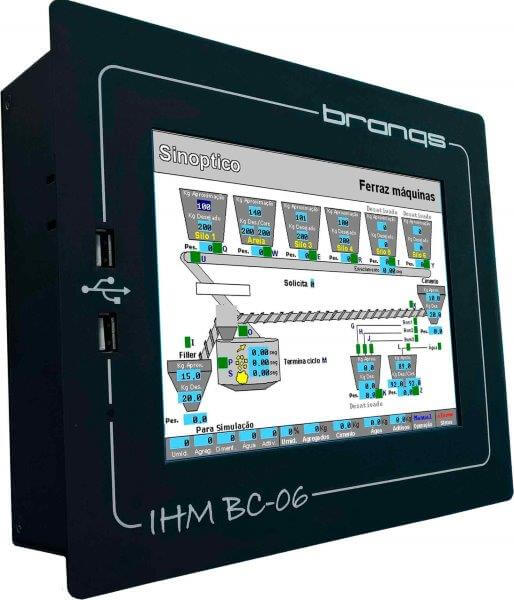
\includegraphics[width=6cm]{figuras/figura-ihm.jpg}}
		}{
			\Fonte{\cite{Branqs}}
		}	
	    \end{figure}
        
    \subsection{Unidade de Aquisição de Dados}
    \label{sec:uad}

        \gls{UAD} são dispositivos que recebem informações relativas ao processo em que estão inseridas e as transferem à um controlador de processo ou diretamente ao sistema de supervisão e controle, onde serão processadas e organizadas para exibição  \cite{mamede-instalacoes}.
        \newpage
        Dividem-se em duas categorias mais específicas:
        
        \begin{alineascomponto}
        	\item \gls{UD}: é um dispositivo inserido dentro do processo em que se mantenha apenas uma função dedicada  \cite{mamede-instalacoes}, como exemplos: relés digitais, intertravamento, etc.
        	\item \gls{UADC}: 
        	tem a função de adquirir dados e controlar ações nos equipamentos respectivos, são compostos por cartões de eletrônicos associados cada um à uma função específica, unidades lógicas, memórias,  entradas e saídas de dados digitais ou analógicos \cite{mamede-instalacoes}. Dentre elas, as mais comuns são: Controlador Lógico Programável e Unidade Terminal Remota.
        \end{alineascomponto}

    \subsubsection{Controlador Lógico Programável}
    \label{sec:clp}

       \gls{CLP} é uma \gls{UADC} muito utilizada para controle de equipamentos através de programas desenvolvidos externamente pelo utilizador e nele gravados, simulando à nível de \textit{software} e substituindo: chaves, contatores, temporizadores, relés e outros dispositivos \cite{CLPManual}. Permite a inclusão de cartões eletrônicos para a realização de diferentes tarefas específicas. Possui \gls{IHM}, onde o utilizador pode alterar a programação ou executar tarefas configuradas no \gls{CLP} \cite{mamede-instalacoes}. Na Figura \ref{fig:figura-clp} é apresentado um \gls{CLP} da fabricante WEG, de modelo PLC300 que possui todas as características aqui descritas.
       
        \begin{figure}[!h]
		\Caption{\label{fig:figura-clp} Exemplo de CLP de modelo PLC300 da fabricante WEG.}
		%\centering
		\UFCfig{}{
			\fbox{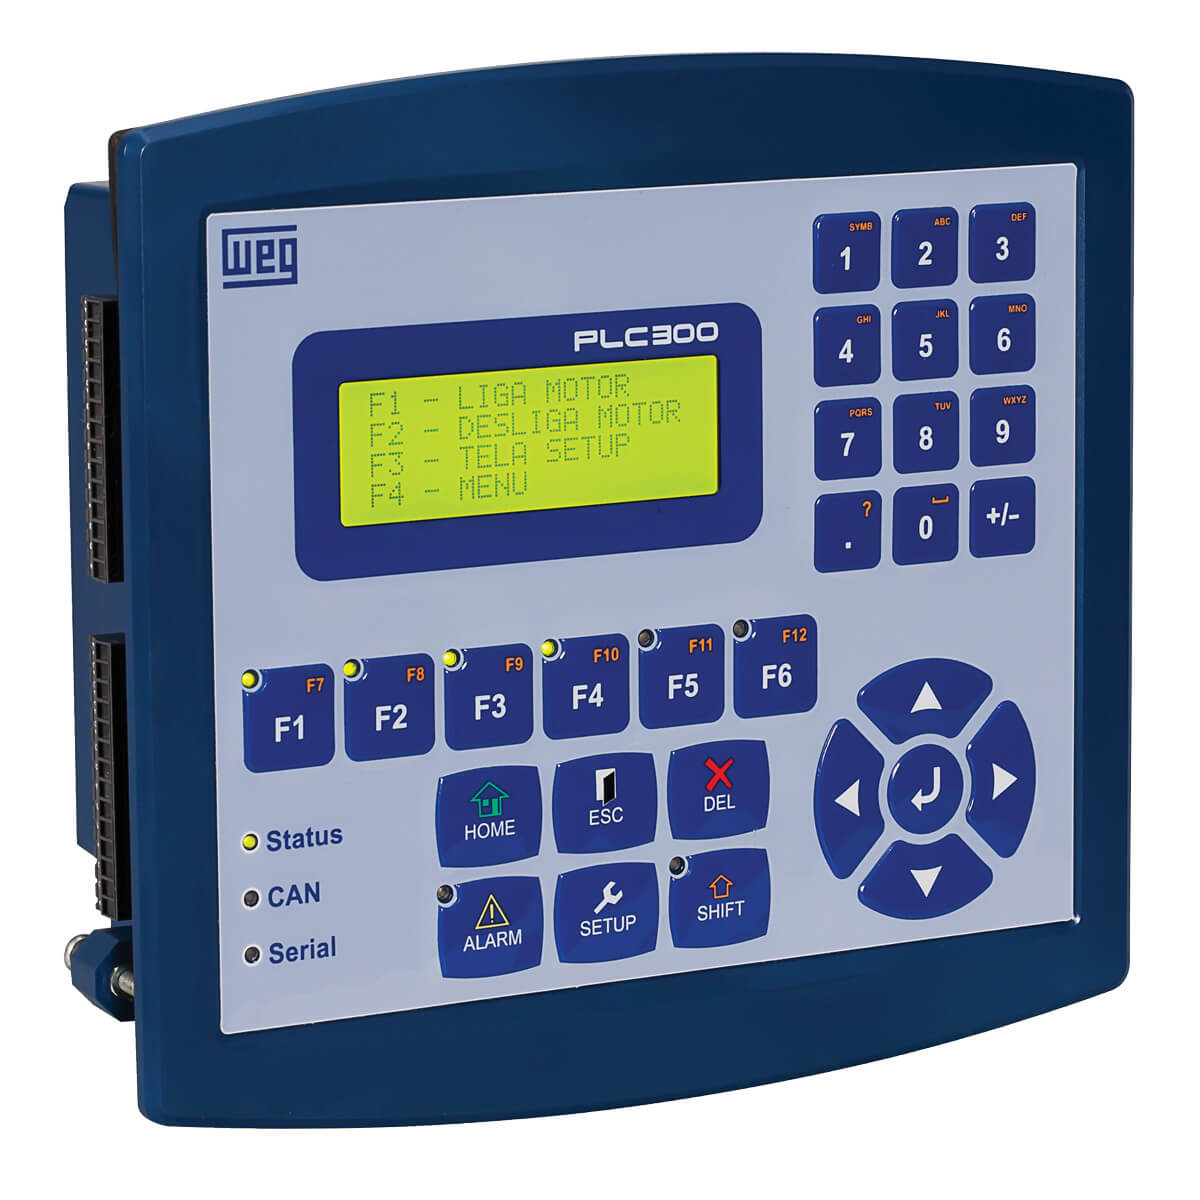
\includegraphics[width=8cm]{figuras/clp-weg.jpg}}
		}{
			\Fonte{\cite{PLC300}.}
		}	
	    \end{figure}
	    
    \subsubsection{Unidade Terminal Remota}
    \label{sec:utr}

       \gls{UTR} é uma \gls{UADC} responsável por coletar informações e executar comandos de equipamentos do processo, sejam eles digitais ou analógicos. Possuem capacidade de executar programas em modo local independente do sistema de supervisão, ao mesmo tempo que possui capacidade de integração com o mesmo. Os comandos locais para equipamentos são feitos através de relés de maneira similar ao que ocorre no \gls{CLP}, por rotinas específicas armazenadas em programas gravados na própria \gls{UTR} \cite{mamede-instalacoes}. Na Figura \ref{fig:figura-utr} é apresentado um \gls{UTR} da fabricante WEG, de modelo RUW-03 que possui todas as características aqui descritas.
       
        \begin{figure}[!h]
		\Caption{\label{fig:figura-utr} Exemplo de UTR de modelo RUW-03 da fabricante WEG.}
		%\centering
		\UFCfig{}{
			\fbox{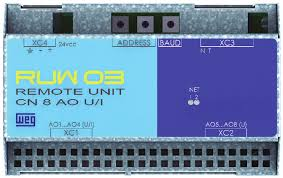
\includegraphics[width=8cm]{figuras/utr-weg.jpg}}
		}{
			\Fonte{\cite{RUW03}}
		}	
	    \end{figure}
      

    \section{Protocolos de Comunicação}
    \label{sec:protocolos}
    A comunicação entre os dispositivos citados na seção anterior e outros, como: sensores, válvulas e atuadores em geral, é essencial para o funcionamento conjunto e ordenado dos mesmos. Desta forma, várias opções foram desenvolvidas ao longo do tempo para tornar a comunicação mais confiável, alguns dos protocolos mais utilizados atualmente são descritos nesta seção.
    
    \subsection{Modbus}
    \label{sec:modbus}
    
    Modbus é um protocolo de comunicação de dados voltado à automação industrial. Desenvolvido em 1979, pela \textit{Modicon}, é até hoje utilizado na indústria em \glspl{CLP} para comandos e aquisição de informações \cite{CLPManual}. Podem ser utilizados os padrões: RS-232, RS-485 ou Ethernet para a camada física de ligação, através de sinais discretos ou analógicos. É geralmente utilizado no tipo mestre-escravo, onde os escravos só enviam comunicação quando solicitadas pelo mestre  \cite{Modbus}.
    
    \subsubsection{Modbus Serial}
    \label{sec:modbus-serial}

        Em redes baseadas em RS-232 e RS-485, a comunicação do Modbus é feita de forma serial através de dois modos distintos: \gls{RTU} e \gls{ASCII}. Na Figura \ref{fig:figura-modbus-serial} são representados as disposições enquanto na Tabela \ref{tab:tabela-modbus-serial} são descritos os pinos da estrutura física RS-485 utilizado pelo Modbus Serial \cite{Modbus}.
        
        No \gls{RTU}, para cada byte transmitido, são codificados em 2 caracteres. Os números variam entre -32768 e 32767, o tamanho da palavra RTU é de 8 bits, organizados conforme a Tabela \ref{tab:tabela-modbus-rtu}. No \gls{ASCII}, os dados são codificados com base na tabela \gls{ASCII}, em que cada byte é transmitido através de dois caracteres. O tamanho da palavra ASCII é de 7 bits, utilizando-se caracteres de intervalos 0-9 ou A-F e entre duas mensagens, 3-5 caracteres, organizados conforme a Tabela \ref{tab:tabela-modbus-ascii}.
        
        \begin{table}[h!]	
        	\centering
        	\Caption{\label{tab:tabela-modbus-rtu} Representação do pacote no modo RTU.}	
        	\IBGEtab{}{
        		\begin{tabular}{crrrr}
        			\toprule
        			Endereço Escravo & Código Função & Dados & CRC \\
        			\midrule \midrule
        			1 byte & 1 byte & 0 a 252 bytes & 2 bytes (CRC-16) \\
        			\bottomrule
        		\end{tabular}
        	}{
        	\Fonte{\cite{Modbus}.}
        }
        \end{table}
        
        \begin{table}[h!]	
        	\centering
        	\Caption{\label{tab:tabela-modbus-ascii} Representação do pacote no modo ASCII.}	
        	\IBGEtab{}{
        		\begin{tabular}{crrrrrr}
        			\toprule
        			Início & Endereço & Função & Dados & LRC & Final \\
        			\midrule \midrule
        			":" & 2 caracteres & 2 caracteres & 0 a 2 x 252 caracteres & 2 caracteres & CR+LF \\
        			\bottomrule
        		\end{tabular}
        	}{
        	\Fonte{\cite{Modbus}.}
        }
        \end{table}
        
        \begin{figure}[!h]
		\Caption{\label{fig:figura-modbus-serial} Pinagem do conector RS485 utilizado no protocolo Modbus Serial.}
		%\centering
		\UFCfig{}{
			\fbox{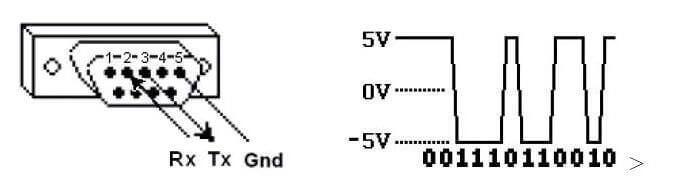
\includegraphics[width=10cm]{figuras/modbus.jpg}}
		}{
			\Fonte{se.com - Acessado em: 28/03/2019}
		}	
	    \end{figure}
	    
	   \begin{table}[h!]	
        	\centering
        	\Caption{\label{tab:tabela-modbus-serial} Pinagem do conector RS485 utilizado no protocolo Modbus Serial.}	
        	\IBGEtab{}{
        		\begin{tabular}{crrrrrr}
        			\toprule
        			Pino &&&&& Sinal \\
        			\midrule \midrule
        			1 &&&&& Não conectado \\
        			2 &&&&& RX - Recepção \\
        			3 &&&&& TX - Envio \\
        			4 &&&&& Não conectado \\
        			5 &&&&& Gnd - Terra \\
        			6 &&&&& Não conectado \\
        			7 &&&&& Não conectado \\
        			8 &&&&& Não conectado \\
        			9 &&&&& Não conectado \\
        			\bottomrule
        		\end{tabular}
        	}{
        	\Fonte{Adaptado de se.com - Acessado em: 28/03/2019}
        }
        \end{table}
        
    \subsubsection{Modbus TCP/IP}
    \label{sec:modbus-tcp}

        As redes baseadas em Ethernet, sob o protocolo \gls{TCP/IP}, foram desenvolvidas para a substituição do Serial devido a simplicidade de seus conectores e uso. O \gls{TCP/IP} é um conjunto de protocolos em camadas, que oferece confiabilidade no transporte de dados entre máquinas, e devido à isso, este padrão torna-se uma opção ideal para sistemas empresariais corporativos. O Modbus \gls{TCP/IP} tornou-se muito utilizado devido sua simplicidade e baixo custo, demandando \textit{hardwares} mínimos para ser utilizado. A maioria dos dispositivos Modbus atualmente presentes no mercado, suportam o padrão \gls{TCP/IP}, aumentando a cada ano a disponibilidade. Há também a possibilidade de conversão entre TCP/IP e Serial, onde é possível garantir a retrocompatibilidade entre dispositivos. Na Figura \ref{fig:figura-modbus-ethernet} é apresentada a pinagem e na Tabela \ref{tab:tabela-modbus-ethernet}, a caracterização por pino do conector utilizado no Modbus \gls{TCP/IP} \cite{Modbus}.

        
        \begin{figure}[!h]
		\Caption{\label{fig:figura-modbus-ethernet} Pinagem do conector RJ45 utilizado no protocolo Modbus Ethernet.}
		%\centering
		\UFCfig{}{
			\fbox{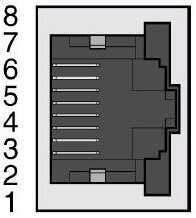
\includegraphics[width=4cm]{figuras/modbus-ethernet.jpg}}
		}{
			\Fonte{Adaptado de se.com}
		}	
	    \end{figure}
	    
        \begin{table}[h!]	
        	\centering
        	\Caption{\label{tab:tabela-modbus-ethernet} Pinagem do conector RJ45 utilizado no protocolo Modbus Ethernet.}	
        	\IBGEtab{}{
        		\begin{tabular}{crrrrrr}
        			\toprule
        			Pino &&&&& Sinal \\
        			\midrule \midrule
        			1 &&&&& CAN\_H \\
        			2 &&&&& CAN\_L \\
        			3 &&&&& CAN\_GND \\
        			4 &&&&& D1 - RS485 (Modbus) \\
        			5 &&&&& D0 - RS485 (Modbus) \\
        			6 &&&&& Não conectado \\
        			7 &&&&& VP - Reservado ao conversor RS232/RS485 \\
        			8 &&&&& Comum \\
        			\bottomrule
        		\end{tabular}
        	}{
        	\Fonte{Adaptado de se.com - Acessado em: 28/03/2019}
        }
        \end{table}

        
    \subsection{OPC}
    \label{sec:opc}
    
        \gls{OPC}, inicialmente chamado \textit{Object Linking and Embedding for Process Control}, desenvolvido pela \textit{OPC Foundation} em 1996 e gerenciado por esta desde então, o \gls{OPC} é o padrão de interoperabilidade para o transporte seguro e confiável de informações no espaço industrial, ele é independente de plataforma e garante o fluxo contínuo de informações entre dispositivos de vários fornecedores. É uma série de especificações desenvolvidas por fornecedores do setor, usuários e desenvolvedores. Essas especificações definem a interface entre Clientes e Servidores, bem como Servidores e Servidores, incluindo acesso a dados em tempo real, monitoramento de alarmes e eventos, acesso a dados históricos e outros aplicativos. \cite{OPC}
        
        Seu propósito inicial era agregar vários outros tipos de protocolos distintos de \glspl{CLP}, proprietários ou não, como: Modbus (seção \ref{sec:modbus}), Profibus, etc, de forma simplificada, através de comunicação genérica, permitindo então, que os usuários implementassem sistemas usando os melhores produtos, interagindo perfeitamente via \gls{OPC}.

    \subsubsection{OPC Classic}
    \label{sec:opc-classic}

        Inicialmente, o padrão \gls{OPC} era restrito e baseado na plataforma \textit{Windows}, utilizando \gls{COM/DCOM} para a comunicação entre \textit{softwares}. Como visto na sigla original do \gls{OPC}, ele era suportado por \gls{OLE} voltado à Controle de Processo, essas especificações, agora conhecidas como \gls{OPC} \textit{Classic}, tiveram ampla adoção em vários setores \cite{OPCClassic}. Na Figura \ref{fig:figura-opc-classic} é representado o funcionamento de um sistema que utilize \gls{OPC} \textit{Classic}, onde o Servidor \gls{OPC} recebe informações de inúmeros módulos de aquisição de dados, de diferentes fabricantes e diferentes protocolos e permite a interoperabilidade deles com o Cliente \gls{OPC}, de forma genérica.
                
        \begin{figure}[!h]
		\Caption{\label{fig:figura-opc-classic} Diagrama do funcionamento de um sistema que utilize OPC Classic.}
		%\centering
		\UFCfig{}{
			\fbox{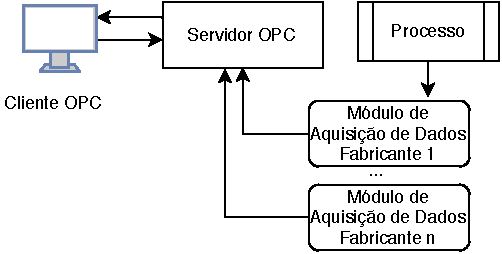
\includegraphics[width=10cm]{figuras/opc.pdf}}
		}{
			\Fonte{O autor}
		}	
	    \end{figure}
	    
	    \quad
	    
	    Existem três definições principais:
        
        \begin{alineascomponto}
        	\item Acesso a Dados - \textit{\gls{OPC} Data Access (DA)}: onde ocorrem troca de dados, incluindo valores, tempo e informações de qualidade.
        	\item Alarmes e Eventos - \textit{\gls{OPC} Alarms \& Events (AE)}: para troca de mensagens de alarmes e tipos de eventos, estados de variáveis e gerenciamento de estados.
        	\item Acesso a Dados Históricos - \textit{\gls{OPC} Historical Data Access (HDA)}: define os métodos de consulta e quais análises podem ser aplicadas a dados históricos, com registro de data e hora.
        \end{alineascomponto}

    \subsubsection{OPC-UA}
    \label{sec:opc-ua}

        Com a introdução de arquiteturas orientadas a serviços em sistemas de manufatura, surgiram novos desafios em segurança e modelagem de dados, a \textit{OPC Foundation} desenvolveu as especificações do \gls{OPC-UA} em 2008, sendo uma arquitetura orientada a serviços independentes, aberta e escalável. Na Figura \ref{fig:figura-opc-ua} é representado um diagrama sobre seu funcionamento.
        
	    \begin{figure}[!h]
		\Caption{\label{fig:figura-opc-ua} Diagrama do funcionamento de um sistema que utilize OPC-UA.}
		%\centering
		\UFCfig{}{
			\fbox{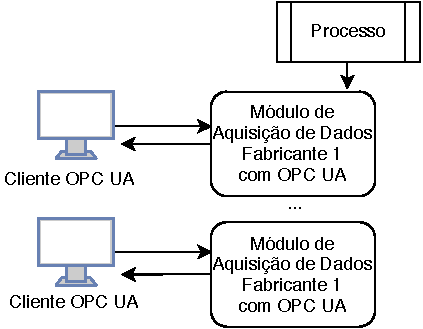
\includegraphics[width=8cm]{figuras/opc-ua.pdf}}
		}{
			\Fonte{O autor}
		}	
	    \end{figure}
        
        O \gls{OPC-UA} integra todas as funcionalidades do \gls{OPC} \textit{Classic}, além de outras melhorias, como:
        
        \begin{alineascomponto}
        	\item Segurança: criptografia de 128 ou 256 bits, verificação de erros para que a mensagem recebida seja exatamente a mensagem enviada, autenticação através de certificados e níveis de permissão;
        	\item Extensível: é possível adicionar novos recursos mantendo a compatibilidade com aplicações já existentes;
        	\item Descoberta: permite a busca por servidores \gls{OPC} na rede ou em computadores;
        	\item Hierarquia: todos os dados são dispostos de forma hierárquica, permitindo informações simples e complexas na mesma estrutura;
        	\item Auditoria: os dados à serem lidos/escritos possuem permissões de acesso tais como registros sobre sua utilização;
        	\item Independência de plataforma: funciona em computadores tradicionais e servidores em nuvem, seja o sistema operacional \textit{Linux}, \textit{Windows} ou outros, \glspl{CLP}, micro-controladores, etc.
        	
        \end{alineascomponto}
	    
    \subsection{HTTP}
    \label{sec:http}
    \gls{HTTP}, coordenado pela \gls{W3C}, é um protocolo de comunicação à nível de aplicação para distribuição de informação de hipermídia, é base para comunicação pela \gls{WEB} desde 1990. Inicialmente, em sua versão HTTP/0.9, era um simples protocolo de transferência de dados não tratados através da Internet e em sua versão atual HTTP/1.1, lançado em 1999, foram implementadas outras funcionalidades como a possibilidade de troca de mensagens no formato \gls{MIME}, que carregam consigo metainformações sobre a requisição ou resposta e o corpo das informações transferidas \cite{HTTP}.
    
    A transferência de informação acontece através de \textit{sockets} sob o protocolo \gls{TCP/IP}, onde com a arquitetura cliente-servidor, o cliente envia uma requisição ao servidor, com o padrão \gls{MIME} e  localizado através endereços, como o \gls{URI}, que identifica a informação acessada e \gls{URL}, que determina a localização desta informação, a conexão é completada e o servidor retorna o \textit{status} de acordo com o sucesso ou não da requisição e possíveis conteúdos também em formato \gls{MIME} caso sejam necessários, encerrando assim a conexão.
    
        \subsubsection{HTTPS}
        \label{sec:https}
        O \gls{HTTPS} é uma derivação do protocolo de comunicação \gls{HTTP} para mensagens seguras, projetado como uma camada de segurança utilizando o protocolo \gls{TLS}. Além de fornecer uma variedade de mecanismos de segurança para clientes e servidores, não são necessárias chaves públicas do lado cliente, suporta criptografia ponta a ponta e torna possível verificar a autenticidade do servidor através de certificados digitais. Seu uso é recomendado em redes inseguras, evitando a clonagem das informações trafegadas que poderia acontecer na ausência de criptografia \cite{HTTPS}. Segundo \cite{usoHTTPS}, em fevereiro de 2019, mais de 58.44\% dos 1 milhões \textit{websites} mais visitados da internet já utilizavam o \gls{HTTPS}.
        
        \subsubsection{REST}
        \label{sec:rest}

        O \gls{REST} é um estilo de arquitetura para \textit{\gls{WEB} Service},  uma solução padronizada pela \gls{W3C} e \gls{OASIS} que busca fornecer interoperabilidade entre dispositivos e aplicações pela internet utilizando diferentes tipos de linguagens, o que a torna compatível com a maioria das aplicações já existentes \cite{W3C}.
        
        O envio e recebimento das mensagens é realizada de forma simplificada através dos protocolos \gls{HTTP} ou \gls{HTTPS} utilizando os formatos: \gls{XML}, \gls{JSON} ou \gls{HTML} e métodos de chamada bem definidos: GET, POST, PUT, PATCH e DELETE. Comumente utilizado por empresas no o desenvolvimento de \gls{API} para acesso a informações específicas sobre serviços, aplicações, faturas, etc. Na Figura \ref{fig:figura-rest1} é apresentada uma ideia geral sobre o funcionamento de uma API que utiliza a arquitetura REST para troca dos dados.
            
            \begin{figure}[!h]
    		\Caption{\label{fig:figura-rest1} Representação do funcionamento de uma API REST.}
    		%\centering
    		\UFCfig{}{
    			\fbox{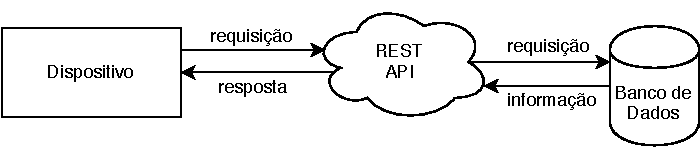
\includegraphics[width=15cm]{figuras/figura-rest1.pdf}}
    		}{
    			\Fonte{O autor}
    		}	
    	    \end{figure}
    	
    	\subsubsection{Métodos de Chamada}
    	\label{sec:metodos-chamada}
    	
    	Quando uma nova requisição é feita, é necessário definir o método que será utilizado. Os métodos de chamada são padronizados para o protocolo \gls{HTTP} e são conhecidos como verbos, pois identificam a ação que será executada pela requisição. Na Tabela \ref{tab:tabela-metodos-chamada} é apresentado um comparativo resumido sobre os métodos de chamada apresentados. Os mais comuns são:
    	
        \begin{alineascomponto}
        	\item GET: apenas recebe informações, as requisições devem ser seguras e idempotentes, ou seja, independente de quantas vezes ela seja repetida, com os mesmos parâmetros, o resultado sempre deve ser o mesmo. Podem haver solicitações parciais ou condicionais;

            \item POST: envia e recebe informações, é utilizado na criação de novos "objetos"\: (elementos da aplicação), mas também é comum o uso para atualização destes;
            
            \item PUT: envia e recebe informações, é utilizado na atualização de "objetos"\: já existentes, na falta do envio de algumas informações necessárias, estas são considerados nulas ou vazias. Assim como o GET, o PUT é idempotente;
            
            \item PATCH: envia e recebe de informações, similar ao PUT,  é utilizado na atualização de "objetos"\: já existentes, porém, apenas os campos especificados;

            \item DELETE: envia e recebe de informações, é utilizado na exclusão de "objetos", podendo ser imediato ou não.
        \end{alineascomponto}
        
       
        
        \begin{table}[h!]	
        	\centering
        	\Caption{\label{tab:tabela-metodos-chamada} Comparativo entre os métodos de chamada.}	
        	\IBGEtab{}{
        		\begin{tabular}{crrrr}
        			\toprule
        			Método & Descrição & Seguro & Idempotente \\
        			\midrule \midrule
        			GET & Recebe informações & sim & sim \\
        			POST & Cria objetos & não & não \\
        			PUT & Atualiza objetos, na falta de informações, considera como nulas & não & sim \\
        			PATCH & Atualiza objetos, alterando apenas as informações enviadas & não & não \\
        			DELETE & Exclui objetos, imediatamente ou não & não & sim \\
        			\bottomrule
        		\end{tabular}
        	}{
        	\Fonte{O autor}
        }
        \end{table}

    	\subsubsection{Formatos de Conteúdo}
    	\label{sec:formatos-de-conteudo}
    	São tipos de linguagem de marcação para necessidades especiais com a finalidade de transferência de informações pela internet. Os mais comuns são:
    	
        \begin{alineascomponto}
        	\item \gls{HTML}: é o formato de texto puro definido em requisições do protocolo \gls{HTTP}.
            \item \gls{XML}:  é baseado em texto simples, de simples leitura, pode representar listas, registros e árvores. Seu próprio formato descreve sua estrutura, campos e valores, os dados são organizados de forma hierárquica e é editável em qualquer ambiente \cite{XML}. Na Figura \ref{fig:figura-xml} é apresentado um exemplo de utilização do formato \gls{XML}.

            \item \gls{JSON}: é um formato leve de informações, de simples leitura e análise. Assim como o \gls{XML} é hierárquico, em pares, ou seja, para cada rótulo, há um valor associado ou sub-conjunto destes. Na Figura \ref{fig:figura-json} é apresentado um exemplo de utilização do formato \gls{JSON} \cite{JSON}.
            
                \begin{figure}[!h]
        		\Caption{\label{fig:figura-xml} Exemplo de informações organizadas no formato XML.}
        		%\centering
        		\UFCfig{}{
        			\fbox{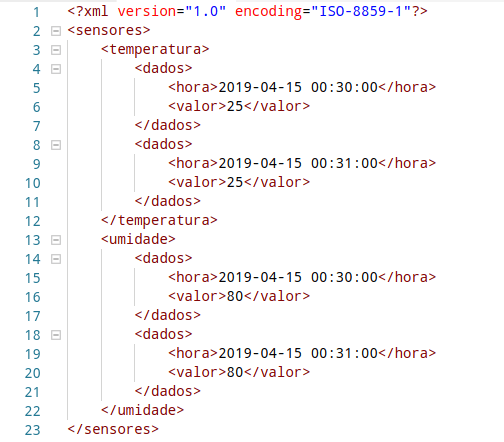
\includegraphics[width=12cm]{figuras/exemploXML.png}}
        		}{
        			\Fonte{O autor}
        		}	
        	    \end{figure}
            
                \begin{figure}[!h]
        		\Caption{\label{fig:figura-json} Exemplo de informações organizadas no formato JSON.}
        		%\centering
        		\UFCfig{}{
        			\fbox{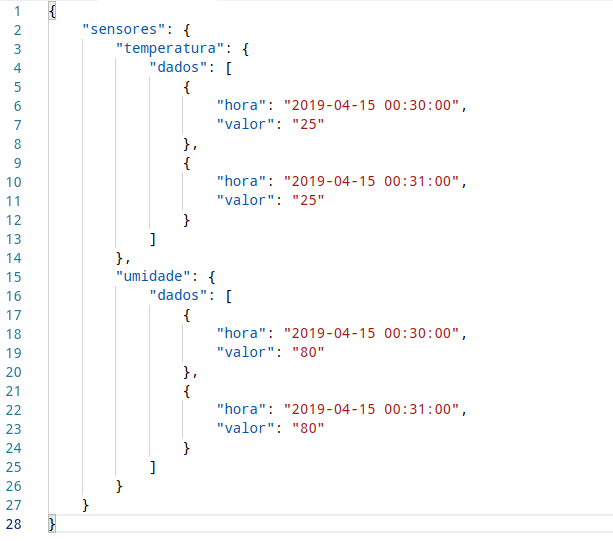
\includegraphics[width=12cm]{figuras/exemploJSON.png}}
        		}{
        			\Fonte{O autor}
        		}	
        	    \end{figure}
        \end{alineascomponto}

    \subsection{MQTT}
    \label{sec:mqtt}

        O \gls{MQTT} foi desenvolvido por Dr. Andy Stanford-Clark, da IBM, e Arlen Nipper, da Arcom no ano de 1999. É um protocolo de mensagens extremamente simples e leve, projetado para ser utilizado em dispositivos que tenham restrição de largura de banda, alta latência ou baixa confiabilidade. Baseia-se na topologia publicador/assinatura, onde as mensagens são enviadas com identificação através de tópicos (\textit{topics}) ou sub-tópicos, o que permite uma única mensagem ser destinada à múltiplos receptores com apenas um envio, ou da mesma forma, receber informações agrupadas de vários sub-tópicos. O elemento responsável pelo envio e recebimento de mensagens é denominado \textit{broker}, que funciona como uma central, intermediando as informações enviadas pelos dispositivos e aplicações da rede \cite{MQTT}. Na Figura \ref{fig:figura-mqtt1} é apresentado     um exemplo de utilização ao qual um subscritor (possível dispositivo associado à rede) recebe informações de dois sensores utilizando um único tópico.
        
        \begin{figure}[!h]
		\Caption{\label{fig:figura-mqtt1} Representação do funcionamento do MQTT.}
		%\centering
		\UFCfig{}{
			\fbox{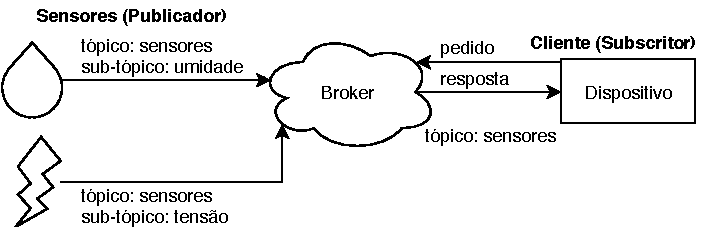
\includegraphics[width=15cm]{figuras/figura-mqtt1.pdf}}
		}{
			\Fonte{O autor}
		}	
	    \end{figure}
	    \newpage
	    A autenticação é feita através de usuário e senha, com a possibilidade de conexão criptografada e a escolha de três níveis de serviço (prioridades na transmissão) que dependerá do projeto em questão, qualidade de conexão do dispositivo, entre outros, sendo elas: 
	    
        \begin{alineascomponto}
        	\item Nível 0: não é feita quaisquer confirmações sobre a entrega da informação, de forma que a mensagem é descartada após o envio.
        	\item Nível 1: são feitas várias tentativas de entrega até que se obtenha confirmação no recebimento, mesmo que isso implique no recebimento em duplicidade.
        	\item Nível 2: há garantia de que a mensagem só será entregue uma vez, havendo tanto a confirmação de entrega da mensagem como a confirmação da confirmação de entrega.
        \end{alineascomponto}

\section{Síntese}
\label{sec:sintese-dispositivos-protocolos}

Neste capítulo são introduzidos os principais dispositivos e protocolos utilizados na indústria para atuação ou aquisição de dados referentes ao processo. Formatos de dados e outros conceitos aqui descritos, serão utilizados nos capítulos seguintes para entendimento da proposta deste trabalho.
	\chapter{Sistemas SCADA}
\label{chap:scada}

    Sistemas de Supervisão e Aquisição de Dados, do inglês, \gls{SCADA}, consistem basicamente de \textit{softwares} que monitoram e operam partes de um ou mais processos, através de unidades de aquisição de dados, como o \gls{CLP}, que por sua vez, conectado fisicamente ao servidor \gls{SCADA} e aos atuadores, utiliza protocolos de comunicação como os citados na seção \ref{sec:automacao-industrial} para obtenção e armazenamento destas informações. Com o domínio sobre as informações do processo, esta ferramenta é capaz de apresentar através de uma \gls{IHM} e de forma simplificada, valores e estados gerais do processo que se deseja atuar, desta forma, obtêm-se um maior controle sobre a tarefa, pois é possível centralizar a leitura de todos os sensores atuantes, a categorização e histórico destes dados, além da priorização de pendências do processo neste único sistema, reduzindo assim a necessidade um maior número de trabalhadores especializados que desempenhem a mesma função. \cite{WhatScada}
    
    O \gls{SCADA} apresenta uma série de vantagens, dentre elas: (i) redução de custos, devido a possibilidade de geração de relatórios detalhados úteis ao planejamento estratégico, evidenciando possíveis vícios do processo produtivo, (ii) maior desempenho na produção, por determinar os valores ótimos de trabalho, (iii) confiabilidade e continuidade, devido a existência de alarmes críticos, ou seja, notificações visuais ao operador, quando alguma variável ou condição do processo esteja em desacordo com o padrão de operação, desta forma, possíveis problemas que ocasionariam uma maior parada na produção, são mitigados com intervenções de forma quase imediata pelo operador caso sejam necessárias, trazendo assim vantagem competitiva.
    
    Todas as informações do processo podem ser coletadas e armazenadas em tempo real em um banco de dados, podendo serem implementadas no sistema de gestão empresarial da empresa ou utilizadas para cálculos mais complexos, sendo o último realizado por outras máquinas para garantir a que o \gls{SCADA} não tenha seu desempenho prejudicado.
    Uma representação básica do sistema \gls{SCADA} é ilustrada na Figura \ref{fig:figura-scada1}, ao qual todas as informações do processo são centralizadas e exibidas de forma simplificada ao colaborador. 
    
    \begin{figure}[!h]
	\Caption{\label{fig:figura-scada1} Arquitetura física básica do SCADA.}
	%\centering
	\UFCfig{}{
		\fbox{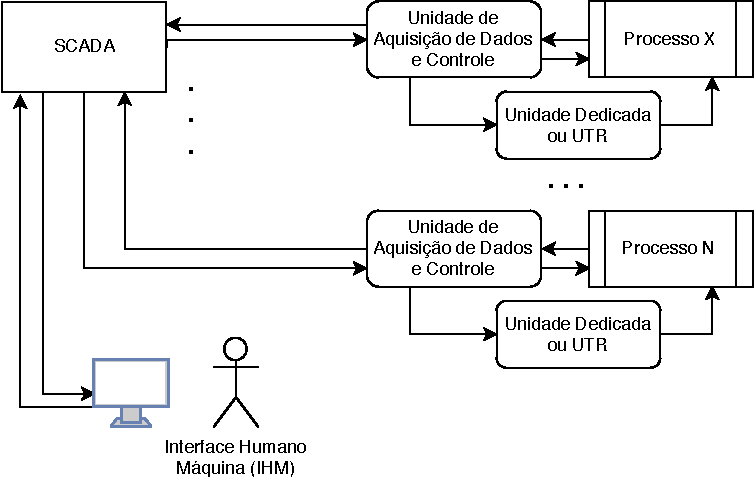
\includegraphics[width=14cm]{figuras/figura-scada1.pdf}}
	}{
		\Fonte{O autor}
	}	
    \end{figure}
    
\section{SCADA WEB}
\label{sec:scadaweb}

Rede Mundial de Computadores (\gls{WEB}), é como se designa o sistema de hiperligações e marcação de texto que permitem a disponibilidade de conteúdo através da \textit{internet}, como: páginas de texto, documentos, músicas, entre outros \cite{W3C}. O \gls{SCADA} \gls{WEB} é uma versão elaborada do SCADA convencional, onde os dados são transferidos para servidores na \textit{internet} e posteriormente processados, integrados às demais plataformas e/ou vistos em páginas WEB. A transição do SCADA para \gls{SCADA} \gls{WEB} ocorre principalmente devido à superação de uma baixa largura de banda e restrições de comunicação como ocorria antigamente. Os avanços tecnológicos possibilitaram a rápida expansão dos canais de dados através da \textit{internet}, onde até mesmo a transmissão de informações em tempo real, não é mais um fator limitante. \cite{ScadaWebSimp}

Sistemas \gls{SCADA} com base na \textit{internet} podem se tornar uma parte importante do funcionamento de sistemas de controle, onde o \gls{XML} e outras formatos disponíveis, podem oferecer possibilidade de resolução de problemas de incompatibilidade que existiam no \gls{SCADA} convencional, onde as fontes de comunicação com o processo são físicas e tornam necessários protocolos de comunicação específicos ou adaptações como o \gls{OPC}. Esta transição também ocorre com os dispositivos utilizados, como \glspl{CLP} e outros, que passam à contar com comunicação \gls{TCP/IP} integrada, alguns deles já com possibilidade de conexão \textit{Wi-Fi}, permitindo a utilização de protocolos como o \gls{HTTP} e \gls{MQTT}, nativos da \gls{WEB}, diretamente do dispositivo, removendo grande parte da camada física. A Figura \ref{fig:figura-clp-wago} traz um exemplo da fabricante WAGO, com uma família de dispositivos que possuem conexão direta à internet, além de recursos de criptografia.

\begin{figure}[!h]
\Caption{\label{fig:figura-clp-wago} Família de Dispositivos com Comunicação Integrada da fabricante WAGO.}
%\centering
\UFCfig{}{
	\fbox{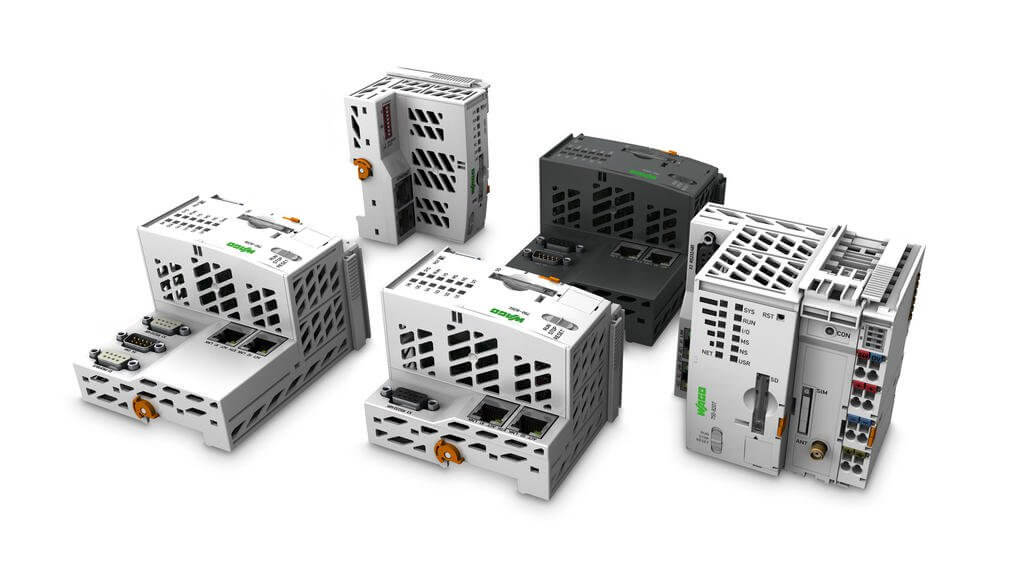
\includegraphics[width=10cm]{figuras/clp-wago.jpg}}
}{
	\Fonte{\cite{WAGO}}
}	
\end{figure}

Independente de como são obtidas as informações, a visualização se dá de forma mais familiar ao usuário, onde antes seria feita através de uma \gls{IHM} física, este ato se reduz à um simples \textit{smartphone} ou página no navegador simulando esta interface, sem ser necessária a instalação de qualquer \textit{software} adicional. A convergência das novas tecnologias, afeta drasticamente a supervisão destas informações, possibilitando controle distribuído e a possibilidade de armazenamento destas informações em qualquer lugar do mundo, com uma ampla capacidade de recursos \cite{ScadaWebInterOp}.

A implementação de um \gls{SCADA} \gls{WEB}, não só abre possibilidade de armazenamento de dados em várias localizações, como também eleva a capacidade de recursos computacionais à um nível muito superior, devido à possibilidade de utilização de servidores em nuvem - interligação de vários servidores através da internet formando um núcleo único de processamento - é possível controlar além de grupos de processos, grupos de plantas em único sistema. Segundo \cite{ScadaNextGer}, a nova geração do \gls{SCADA} pode modificar significamente a forma de projetar e implementar os processos industriais no futuro, onde o sistema terá que lidar com uma quantidade muito superior de dados distribuídos e informações em tempo real para tomar as decisões baseadas neste dados com informações internas e externas. A \gls{IHM} fica não mais limitada à um local físico, mas acessível através de todos os computadores, \textit{smartphones} e \textit{tablets} conectados à \textit{internet}, permitindo a colaboração simultânea na supervisão do processo. Com o uso de várias plantas simultâneamente, há a possibilidade de implementação de uma rotina por prioridades, dependendo das necessidades dinâmicas de cada cliente.  Poucas são as desvantagens de um sistema \gls{SCADA} \gls{WEB}, uma delas, é a perda de robustez do sistema devido as informações e controle serem feitos à distância através da rede, tendo que serem considerados atraso em transporte que, apesar de ser irrisório para a maioria das aplicações, podem chegar a ser um problema para outras. Uma representação básica do sistema \gls{SCADA} \gls{WEB} é ilustrada na Figura \ref{fig:figura-scada-web1}, onde as informações de um grupo de plantas são centralizadas e exibidas de forma simplificada ao colaborador.

    \begin{figure}[!h]
\Caption{\label{fig:figura-scada-web1} Arquitetura de um SCADA WEB.}
%\centering
\UFCfig{}{
	\fbox{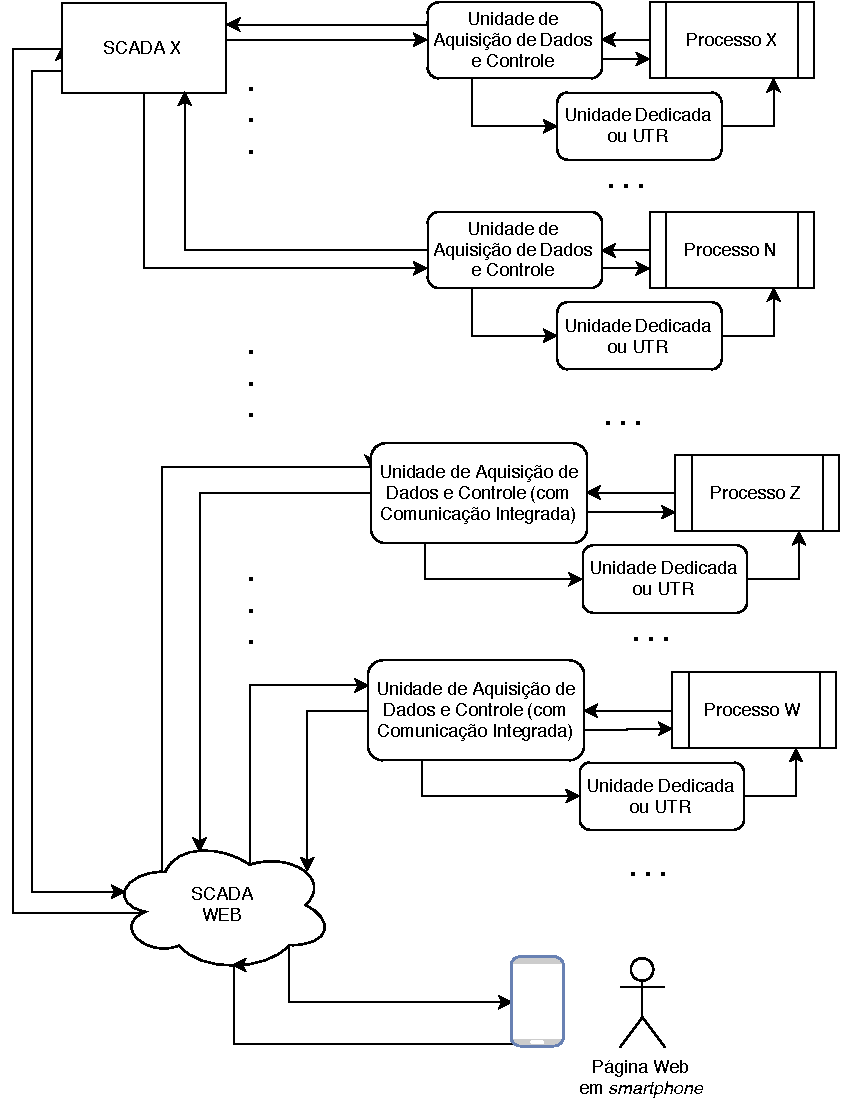
\includegraphics[width=14cm]{figuras/figura-scada-web1.pdf}}
}{
	\Fonte{O autor}
}	
\end{figure}

\section{Sistemas SCADA disponíveis no mercado}
\label{sec:sistemas-scada}

\subsection{Sistemas proprietários}
\label{sec:sistemas-scada-proprietarios}

\subsubsection{Elipse E3}
\label{sec:elipse}

    O Elipse E3 \cite{Elipse}, desenvolvido pela empresa Elipse Software, representa a terceira geração do \gls{SCADA}. Utiliza o conceito de múltiplas camadas, onde incluem: servidores, regras de aplicação ou de negócio e estações clientes. O sistema é composto por 3 aplicações: 
    
    \begin{alineascomponto}
    	\item \textit{E3Server}: é o servidor das aplicações, em que se gerencia todos os processos de execução do \textit{software} e processa a comunicação entre eles. Suas ações são basicamente: envio das informações gráficas e dados para o cliente, gerenciamentos dos processos de E/S e comunicação com os diversos pontos de aquisição, controle da cópia de produtos, cliente e servidor OPC e sincronismo de alarmes e bases de dados. Permite, também, a distribuição deste serviço entre várias máquinas de acordo com a necessidade, com objetivo de manter a continuidade em uma eventual falha.
    	\item \textit{E3Viewer}: responsável pela interface de operação e visualização da aplicação que se encontra no E3Server, com operação local ou via \textit{intranet}/\textit{internet}, pode ser acessado por diversas plataformas como: Mac OS, Linux, Windows CE ou ainda, há a possibilidade de utilização do E3WebServer para gerenciamento adicional do acesso via Internet.
    	\item \textit{E3Studio}: ferramenta para configuração do sistema, servindo como plataforma universal do desenvolvimento. A configuração e execução compartilham da mesma base de dados, de forma que as edições das aplicações podem ser enviadas em \textit{runtime}, sem ser necessário a parada da aplicação, independente de ser feita local ou remotamente. É possível a edição de mais de um aplicativo ao mesmo tempo ou a edição ser feita por mais de uma pessoa devido compartilharem o mesmo servidor. Possui ferramentas, como: editores de telas, relatórios e \textit{scripts}.
    \end{alineascomponto}
    
    \begin{figure}[!h]
	\Caption{\label{fig:figura-elipse-e3} Demonstração da tela de processo do \textit{software} Elipse E3.}
	%\centering
	\UFCfig{}{
		\fbox{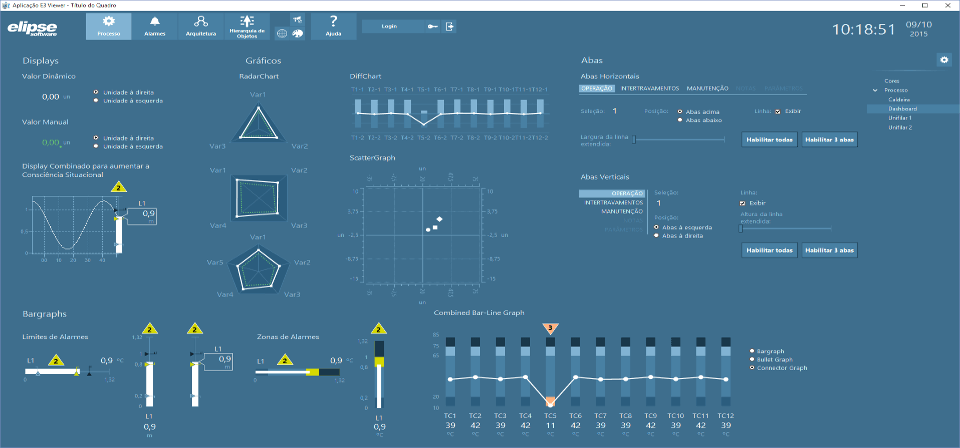
\includegraphics[width=15cm]{figuras/elipse-e3.png}}
	}{
		\Fonte{\cite{Elipse}.}
	}	
    \end{figure}

    
    Outras informações importantes:
    
    \begin{alineascomponto}
    	\item Possui drivers para comunicação com mais de 300 tipos de dispositivos e sistemas, sejam eles proprietários ou \gls{OPC}, além de produzir drivers sob encomenda.
    	\item Possui interfaces específicas para Access (.MDB), SQL Server/MSDE, Oracle ou acesso genérico através de padrões ADO e ODBC, faz acesso à base de dados corporativas fazendo o interfaceamento entre o processo e sistemas administrativos, de produção, manutenção e gestão.
    \end{alineascomponto}
    
\subsubsection{InduSoft Web Studio®}
\label{sec:indusoft}

    O InduSoft Web Studio® \cite{InduSoft}, desenvolvido pela empresa InduSoft, fornece componentes básicos de automação para o desenvolvimento de \glspl{IHM}, sistemas \glspl{SCADA} e soluções de instrumentação embarcada. O sistema é composto por 2 aplicações:
    
    \begin{alineascomponto}
        \item \textit{Server}: é o servidor das aplicações, em que se gerencia todos os processos de execução do \textit{software} e processa a comunicação entre eles. Suas ações são basicamente: envio das informações gráficas e dados para o cliente, gerenciamentos dos processos de entrada e saída,  comunicação com os diversos pontos de aquisição, controle da cópia de produtos, servidor OPC e sincronismo de alarmes e bases de dados.
    	\item \textit{IoTViewer}: responsável pela interface de operação e visualização da aplicação que se encontra no \textit{Server}, com operação local ou via \textit{intranet}/\textit{internet}.
    \end{alineascomponto}

    \begin{figure}[!h]
	\Caption{\label{fig:figura-indusoft} Demonstração da tela de processo do \textit{software} InduSoft Web Studio®.}
	%\centering
	\UFCfig{}{
		\fbox{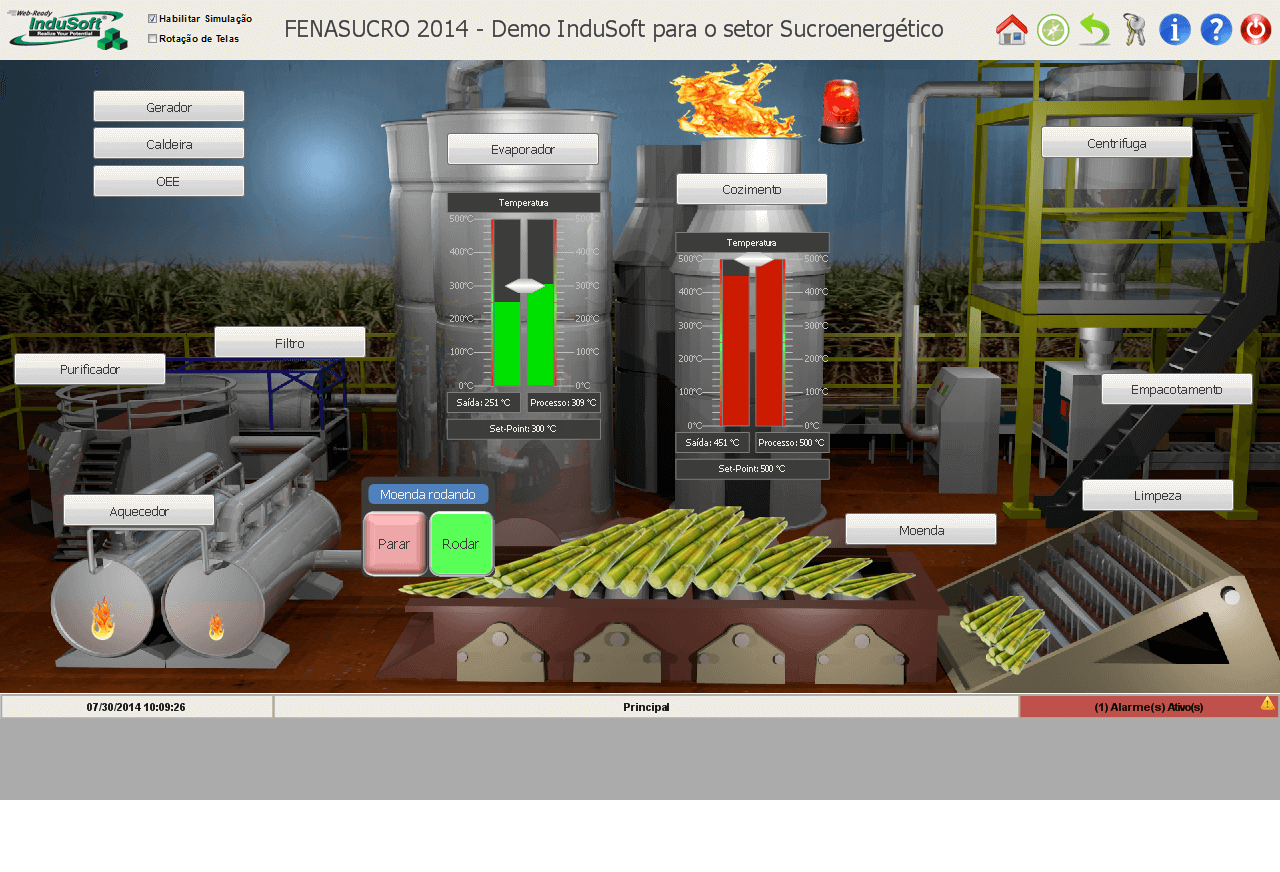
\includegraphics[width=15cm]{figuras/indusoft.png}}
	}{
		\Fonte{\cite{InduSoft}.}
	}	
    \end{figure}
    
    Outras informações importantes:
    
    \begin{alineascomponto}
    	\item A aplicação \textit{Server} suporta as plataformas \textit{Microsoft}, como: \textit{Windows CE, Mobile, XP Embedded e Server}, enquanto a aplicação cliente, o \textit{IoTView}, pode também suportar plataformas, como: \textit{Linux e VXWorks}.
    	\item Permite visualização de processo através de Navegador \gls{WEB}, podendo ser acessado através de celulares ou computadores de mesa, seja em rede local ou pela \textit{internet}.
    	\item Possui suporte para \gls{CLP} ou controlador e drivers para comunicação com mais de 200 tipos de dispositivos e sistemas, sejam eles proprietários ou \gls{OPC}, além de comunicação por \gls{TCP/IP}.
    	\item Alarmes podem ser enviados via \textit{e-mail}, celulares ou através do próprio navegador.
    	\item Permite acesso à base de dados corporativas fazendo o interfaceamento entre o processo e sistemas administrativos, de produção, manutenção e gestão.
    \end{alineascomponto}


\subsection{Sistemas de código aberto}
\label{sec:sistemas-aberto}

\subsubsection{ScadaBR}
\label{sec:scadabr}

    O ScadaBR \cite{ScadaBR} é um \textit{software} livre e de código-fonte aberto. Abrange profissionais de automação, universidades, escolas técnicas e empresas de todos os portes. O projeto foi iniciado em 2006, por iniciativa da empresa MCA Sistemas com sede em Florianópolis - SC, que com o auxílio de outras empresas, a fundação CERTI e a Universidade Federal de Santa Catarina - UFSC, desenvolveram o sistema de forma completa em português baseado no \textit{software} Mango. Possui apoio da FINEP, SEBRAE e CNPq, que também, financiaram a iniciativa durante 2 anos.

    \begin{figure}[!h]
	\Caption{\label{fig:figura-scadabr} Demonstração de telas, incluindo a de processo, do \textit{software} ScadaBR.}
	%\centering
	\UFCfig{}{
		\fbox{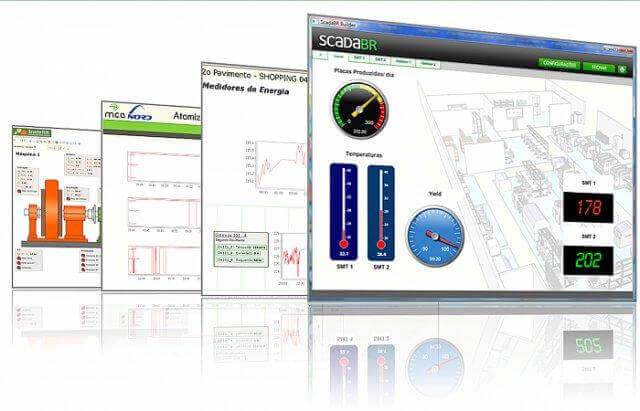
\includegraphics[width=12cm]{figuras/scadabr.jpg}}
	}{
		\Fonte{\cite{ScadaBR}.}
	}	
    \end{figure}
    
    Outras informações importantes:
    
    \begin{alineascomponto}
	    \item A aplicação \textit{Server} suporta diferentes plataformas, como: \textit{Windows} 32/64 bits e \textit{Linux}.
	    \item Permite visualização de processo através de Navegador \gls{WEB}, podendo ser acessado através de celulares ou computadores de mesa, seja em rede local ou pela \textit{internet}.
    	\item Possui mais de 20 protocolos de comunicação, como: Modbus \gls{TCP/IP} e Serial, \gls{HTTP}, etc.
    	\item Customização de \textit{scripts} para controle, automação, etc.
    	\item Possibilidade de cálculos com funções matemáticas, estatísticas etc, com as variáveis do processo.
    	\item Níveis de permissão de usuários, com controle de acesso.
    \end{alineascomponto}
    
\subsubsection{TANGO Controls}
\label{sec:tango}

    O TANGO Controls \cite{Tango} é um \textit{software} livre e de código-fonte aberto. Foi desenvolvido pelo \textit{European Synchrotron Radiation Facility} em Genebra, França e seu desenvolvimento já supera 20 anos de duração. Foi desenvolvido, principalmente, para necessidades de instalações de pesquisas, com o conceito agregado de ser criado um novo \textit{framework}. Pode ser executado de forma autônoma ou distribuída, local ou remota.

    \begin{figure}[!h]
	\Caption{\label{fig:figura-tango} Demonstração da tela de processo do \textit{software} TANGO Controls.}
	%\centering
	\UFCfig{}{
		\fbox{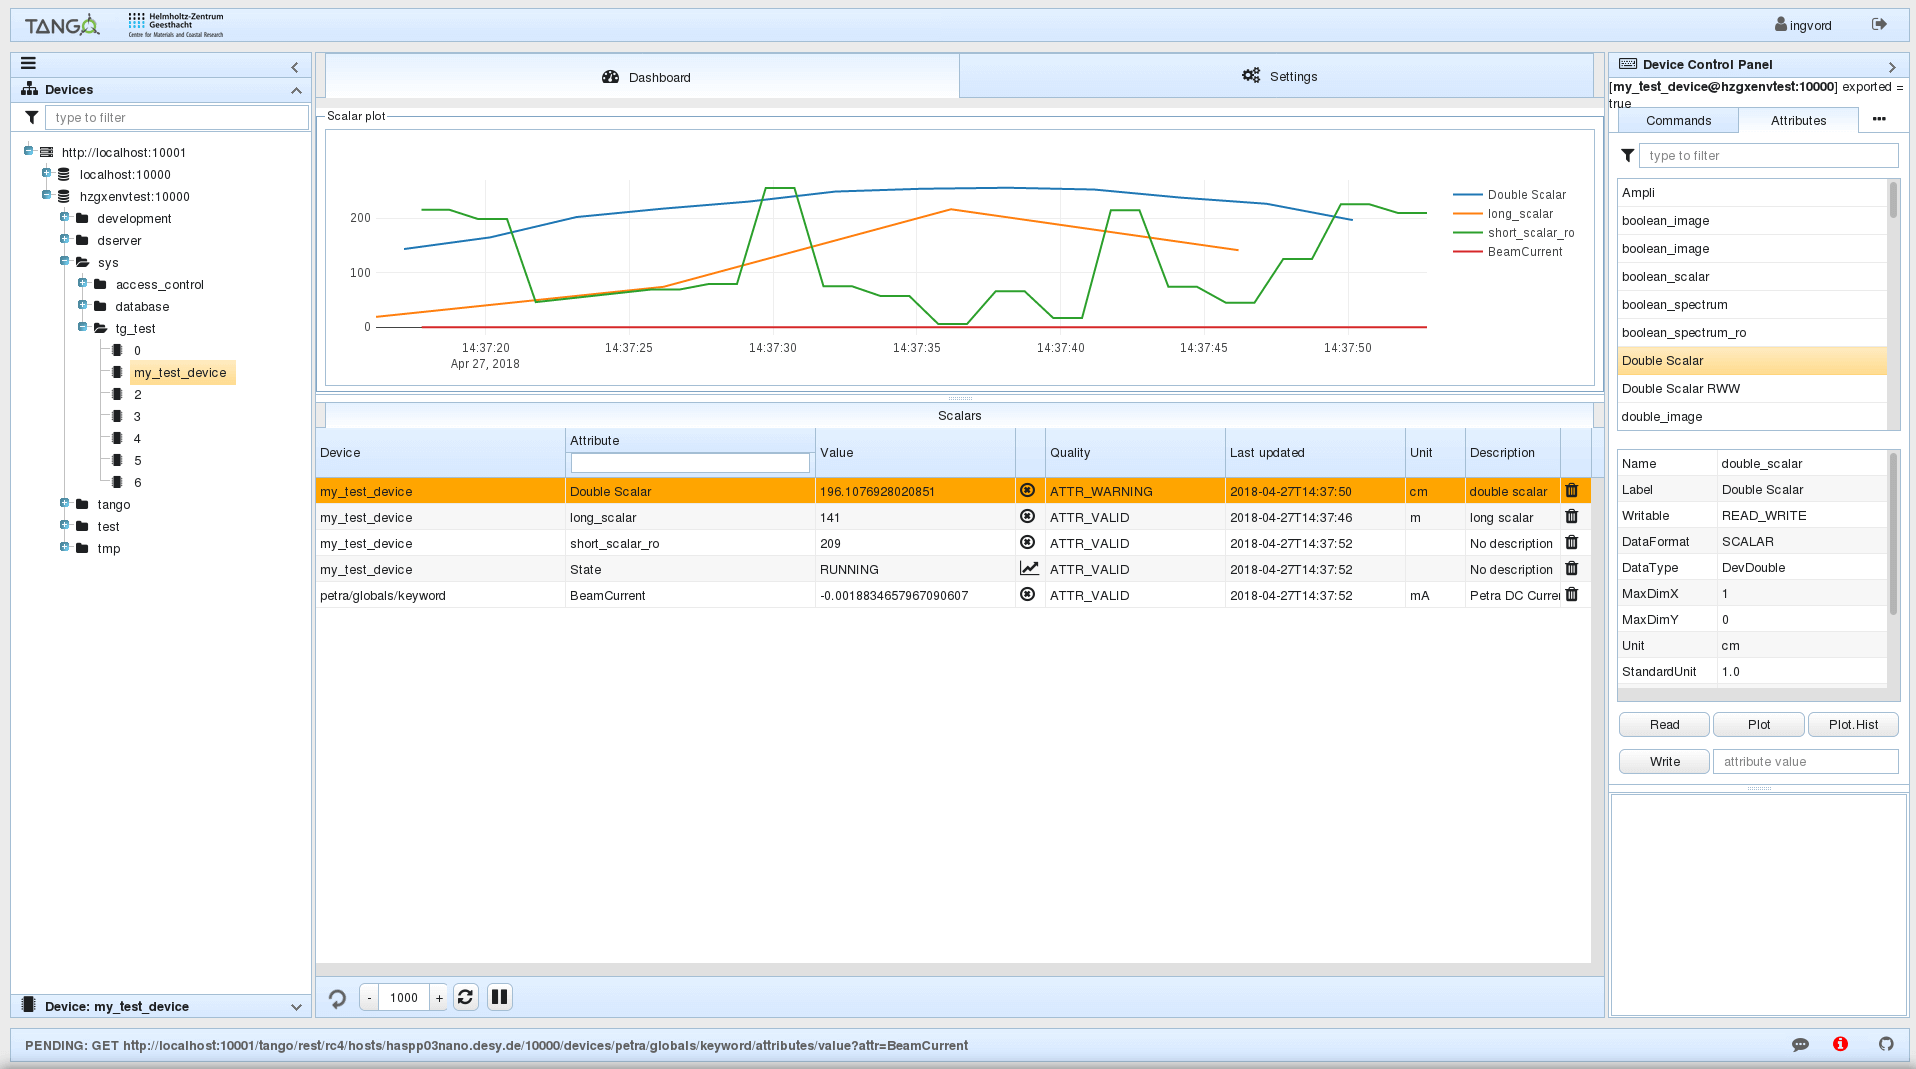
\includegraphics[width=15cm]{figuras/tango.png}}
	}{
		\Fonte{\cite{Tango}.}
	}	
    \end{figure}
    
    Outras informações importantes:
    
    \begin{alineascomponto}
	    \item Permite visualização de processo através de Navegador \gls{WEB}, podendo ser acessado através de celulares ou computadores de mesa, seja em rede local ou pela \textit{internet}.
    	\item Possui diversos \textit{drivers} de comunicação, disponibilizados de forma gratuita.
    	\item Permite a adição de funções analíticas para a tomada de decisões.
    	\item Encontra-se em fase de transição para atender a demanda \textit{IoT} industrial.
    \end{alineascomponto}
    
\subsubsection{Rapid SCADA}
\label{sec:rapidscada}

    O Rapid SCADA \cite{RapidSCADA} é um \textit{software} livre e de código-fonte aberto, desenvolvido pela empresa russa \textit{Rapid Software}.

    \begin{figure}[!h]
	\Caption{\label{fig:figura-rapidscada} Demonstração da tela de processo do \textit{software} Rapid SCADA.}
	%\centering
	\UFCfig{}{
		\fbox{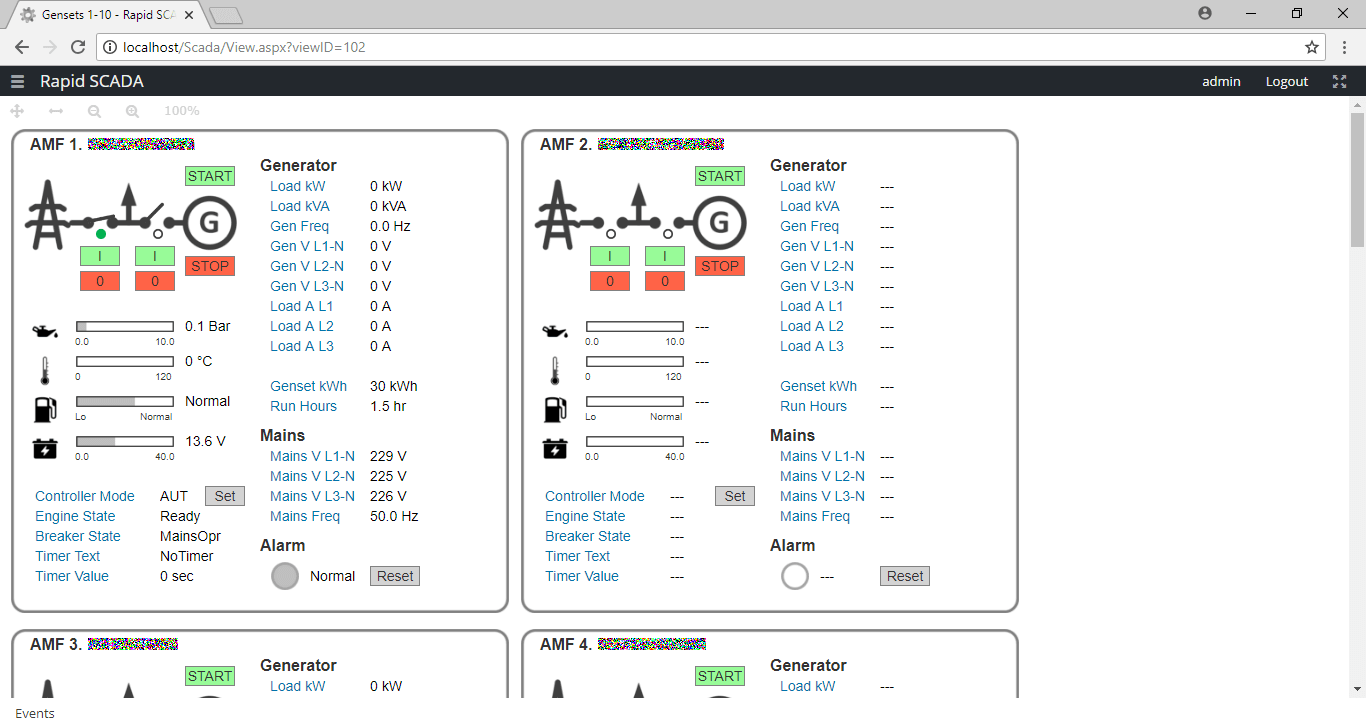
\includegraphics[width=15cm]{figuras/rapidscada.png}}
	}{
		\Fonte{\cite{RapidSCADA}.}
	}	
    \end{figure}
    
    Outras informações importantes:
    
    \begin{alineascomponto}
        \item É suportado por plataformas \textit{Windows} e \textit{Linux}.
	    \item O sistema possui uma interface de administração no modelo cliente/servidor e outra de monitoramento no formato \gls{WEB}.
	    \item Possui \textit{drivers} de comunicação, disponibilizados de forma gratuita, como: Modbus, \gls{OPC}, \gls{MQTT}, etc.
	    \item Níveis de permissão de usuários, com controle de acesso.
	    \item Alarmes de fogo e segurança, com avisos via interface.
	    \item A empresa cobra por serviços de treinamento e suporte na ferramenta, além de comercializar módulos de software adicionais.
    \end{alineascomponto}
    
\section{Síntese}
\label{sec:sintese-scada}

Apresentados os dispositivos e protocolos utilizados na indústria para a manutenção de processos industriais, neste Capítulo foram apresentados os tipos de sistemas \gls{SCADA} existentes assim como os principais \textit{softwares} disponíveis no mercado para esta funcionalidade. Com base em todo o desenvolvimento teórico apresentado, o capítulo seguinte traz a proposta de um sistema \gls{SCADA} baseado em nuvem com a capacidade de gerenciamento de múltiplos projetos na mesma estrutura.
	\chapter{Sistema Desenvolvido}
\label{chap:sistema-desenvolvido}

texto texto texto

\section{Aquisição de Dados}
\label{sec:aquisicao-dados}

    oi
    
    \subsection{Métodos de Aquisição}
    \label{sec:metodos-aquisicao}
        oi
        
        \subsubsection{HTTP}
        \label{sec:aquisicao-http}
        oi
        
        \begin{figure}[!h]
		\Caption{\label{fig:figura-http-geral} Diagrama das etapas do servidor para manipulação de dados.}
		%\centering
		\UFCfig{}{
			\fbox{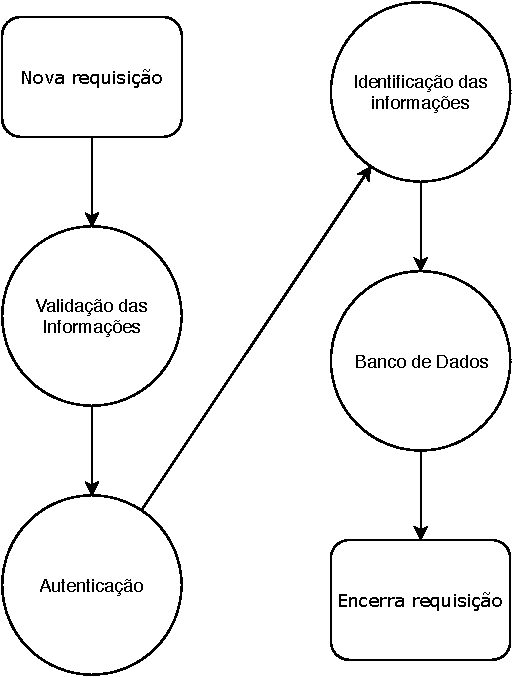
\includegraphics[width=8cm]{figuras/http-geral.pdf}}
		}{
			\Fonte{O autor}
		}	
    	\end{figure}
    	
    	\begin{figure}[!h]
		\Caption{\label{fig:figura-http-validacao} Diagrama de validação das informações recebidas.}
		%\centering
		\UFCfig{}{
			\fbox{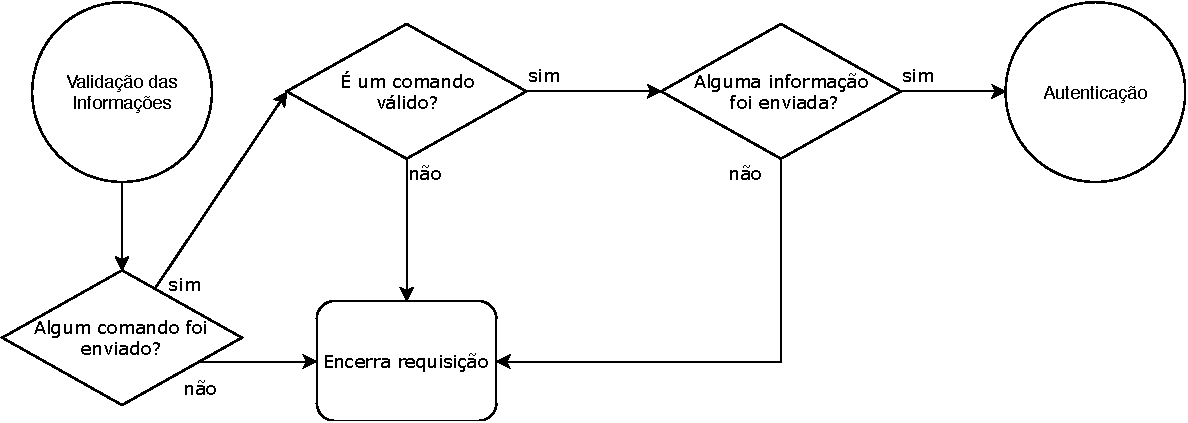
\includegraphics[width=15cm]{figuras/http-validacao.pdf}}
		}{
			\Fonte{O autor}
		}	
    	\end{figure}
    	
    	\begin{figure}[!h]
		\Caption{\label{fig:figura-http-autenticacao} Diagrama de autenticação do usuário.}
		%\centering
		\UFCfig{}{
			\fbox{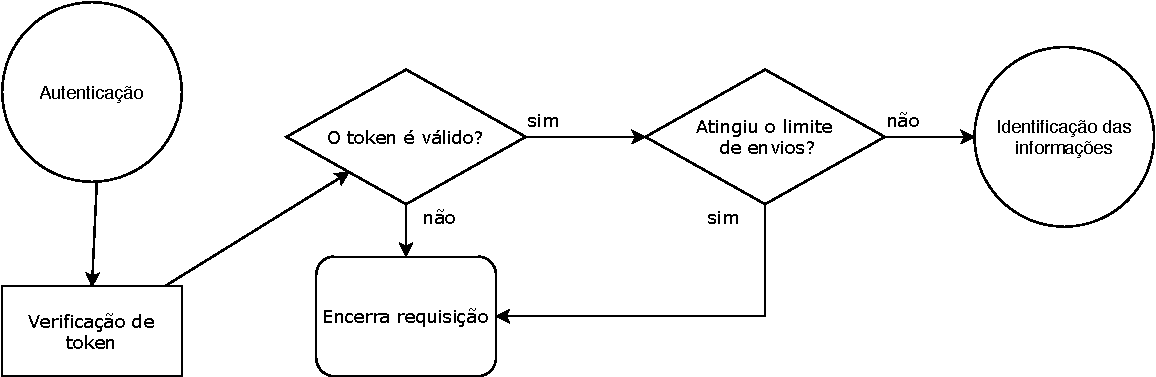
\includegraphics[width=15cm]{figuras/http-autenticacao.pdf}}
		}{
			\Fonte{O autor}
		}	
    	\end{figure}
    	
    	\begin{figure}[!h]
		\Caption{\label{fig:figura-http-identificacao} Diagrama sobre a identificação do tipo das informações.}
		%\centering
		\UFCfig{}{
			\fbox{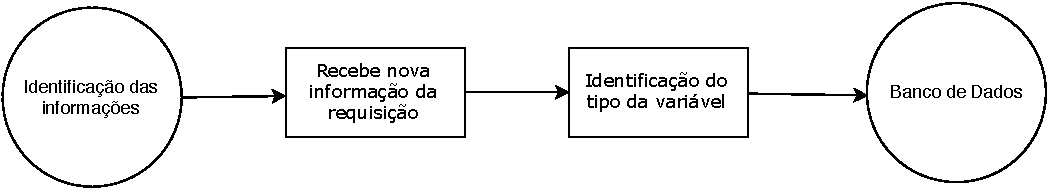
\includegraphics[width=15cm]{figuras/http-identificacao.pdf}}
		}{
			\Fonte{O autor}
		}	
    	\end{figure}
    	
    	\begin{figure}[!h]
		\Caption{\label{fig:figura-http-banco} Banco de Dados.}
		%\centering
		\UFCfig{}{
			\fbox{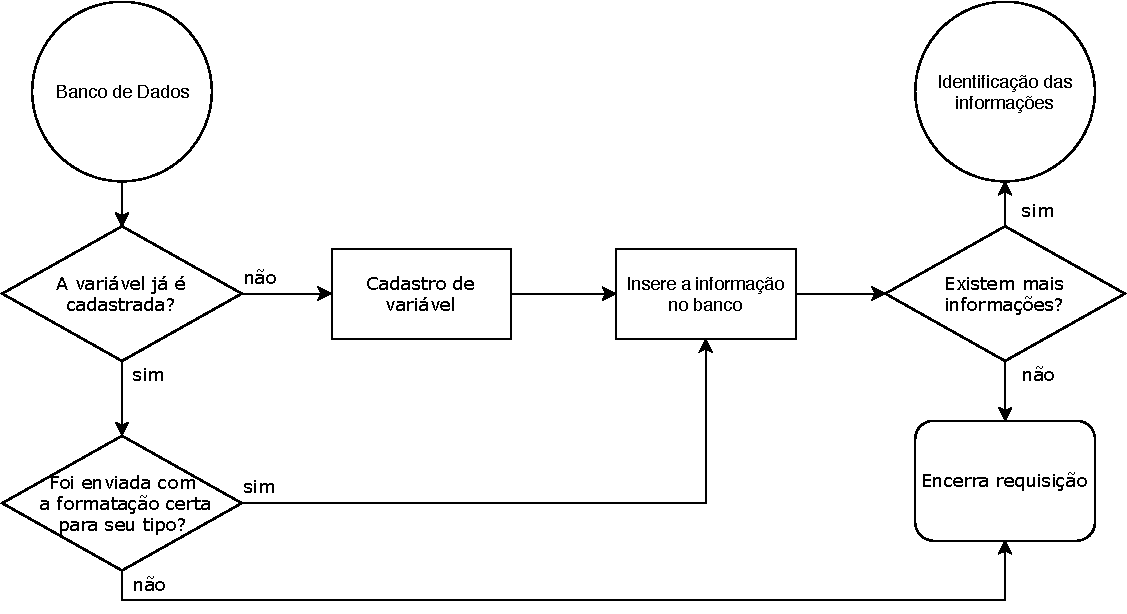
\includegraphics[width=15cm]{figuras/http-banco.pdf}}
		}{
			\Fonte{O autor}
		}	
    	\end{figure}
        
        \subsubsection{MQTT}
        \label{sec:aquisicao-mqtt}
        oi

    \subsection{Armazenamento dos Dados}
    \label{sec:armazenamento-dados}
        oi
        
        \subsubsection{Banco de Dados}
        \label{sec:banco-dados}
        oi
        
        \subsubsection{Tipos de Variáveis}
        \label{sec:tipos-variaveis}
        oi
        
        \subsubsection{Tempo}
        \label{sec:tempo}
        oi
    
\section{Painel de Controle}
\label{sec:painel-controle}
oi
    
    \subsection{Segurança}
    \label{sec:seguranca}
    oi
        
        \subsubsection{Proteções}
        \label{sec:protecoes}
        oi
        
        \subsubsection{Criptografia}
        \label{sec:criptografia}
        oi
        
        \subsubsection{Controle de Acesso}
        \label{sec:controle-acesso}
        oi
        
    \subsection{Projetos}
    \label{sec:projetos}
    oi
    
        \subsubsection{Objetos}
        \label{sec:objetos}
        oi
        
        \subsubsection{Clientes Associados}
        \label{sec:clientes-associados}
        oi
    \subsection{Clientes}
    \label{sec:clientes}
    oi
    
    \subsection{Domínios}
    \label{sec:dominios}
    oi

\section{Recursos Computacionais}
\label{sec:recursos-computacionais }
oi

    \subsection{Armazenamento}
    \label{sec:armazenamento}
    oi
    
    \subsection{Processamento}
    \label{sec:processamento}
    oi

\section{K-NN}
\label{sec:knn}
    \subsection{Classificação}
    \label{sec:classificacao}
    oi
    
    \subsection{Teste}
    \label{sec:teste}
    oi

\section{Plataforma Estudantil}
\label{sec:plataforma-estudantil}
oi

\section{Drivers de Comunicação}
\label{sec:drivers-comunicacao}
oi


	\chapter{Interface de Gerenciamento: rscada}
\label{chap:interface-web}

A interface de gerenciamento foi desenvolvida conforme todos os conceitos descritos no Capítulo \ref{chap:sistema-proposto}, o tema utilizado para estilo da página foi desenvolvido pela empresa Colorlib com código-fonte aberto e modificado à critérios do projeto \cite{Concept}. O nome do sistema, rscada,  foi constituído da inicial R do nome do autor e o tipo do sistema em questão. Todo o código dos módulos foi programado utilizando a linguagem de programação PHP, com exceção da integração entre o banco de dados e o serviço VerneMQ, responsável pelo protocolo MQTT, teve por base programação LUA e os exemplos de utilização da plataforma disponíveis no Capítulo \ref{chap:resultados} que foram desenvolvidos utilizando C++ com pequenas modificações. Todas as etapas e telas do projeto são explicadas abaixo.

\section{Acesso ao Sistema}
\label{sec:acesso-sistema}
Ao acessar a interface de gerenciamento, são solicitados ao utilizador os dados de acesso, sendo eles: usuário ou e-mail e senha. A Figura \ref{fig:figura-rscada-1} traz a tela real de acesso do sistema desenvolvido.

        \begin{figure}[!h]
		\Caption{\label{fig:figura-rscada-1} Tela de autenticação da Interface Web.}
		%\centering
		\UFCfig{}{
			\fbox{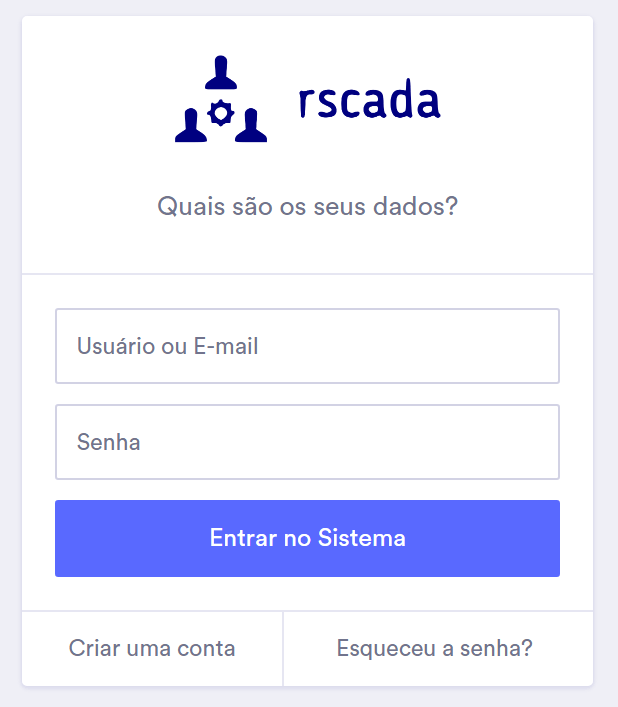
\includegraphics[width=8cm]{figuras/rscada-1.png}}
		}{
			\Fonte{O autor}
		}	
    	\end{figure}

Caso seja um novo utilizador, é fornecido um botão na tela de acesso para criação de novas contas, onde o sistema redirecionará à página de criação de contas e solicitará ao novo usuário: Nome, E-mail, Usuário e Senha, além de uma confirmação de leitura sobre os termos de serviço do rscada. Ao submeter o formulário de criação de nova conta, é enviado ao email do usuário, um \textit{link} contendo um código de confirmação da conta para validar o e-mail digitado. A Figura \ref{fig:figura-rscada-2} demonstra a tela de cadastro para novas contas do rscada.

        \begin{figure}[!h]
		\Caption{\label{fig:figura-rscada-2} Tela de cadastro para novos usuários.}
		%\centering
		\UFCfig{}{
			\fbox{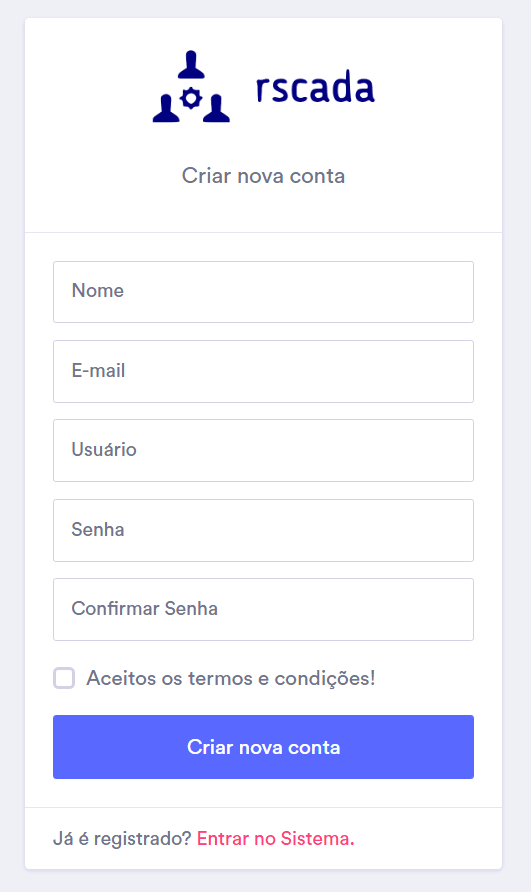
\includegraphics[width=8cm]{figuras/rscada-2.png}}
		}{
			\Fonte{O autor}
		}	
    	\end{figure}

\section{Tela inicial da interface}
\label{sec:tela-inicial}
Devidamente autenticado no sistema, o usuário é redirecionado à tela inicial onde o foco são os projetos cadastrados pertencentes à ele. Informações sobre a quantidade de Clientes associados aos projetos e botões de ações, são disponíveis na página, dentre elas: Novo Projeto, Gerenciamento dos Projetos existentes e Exclusão dos mesmos. Um menu é disponibilizado na lateral esquerda da tela, com os principais atalhos para funções do sistema, como: (i) Minha Conta, onde o usuário poderá alterar detalhes como: E-mail ou Senha, (ii) Meus Projetos, quando necessário retornar à tela inicial dos projetos, (iii) Meus Clientes, para o cadastro de clientes descritos anteriormente como Operadores, que farão uso dos projetos quando desenvolvidos, (iv) Meus Domínios, que o usuário poderá cadastrar o endereço de site o qual os clientes terão acesso ao projeto desenvolvido, (v) Alarmes, para visualizar eventos e alertas de informações que tenham sido inseridas no sistema e que não correspondem aos valores ideiais de funcionamento, entre outros. As Figura \ref{fig:figura-rscada-2} e \ref{fig:figura-rscada-5} trazem capturas da tela descrita.

        \begin{figure}[!h]
		\Caption{\label{fig:figura-rscada-3} Tela inicial do sistema após autenticação.}
		%\centering
		\UFCfig{}{
			\fbox{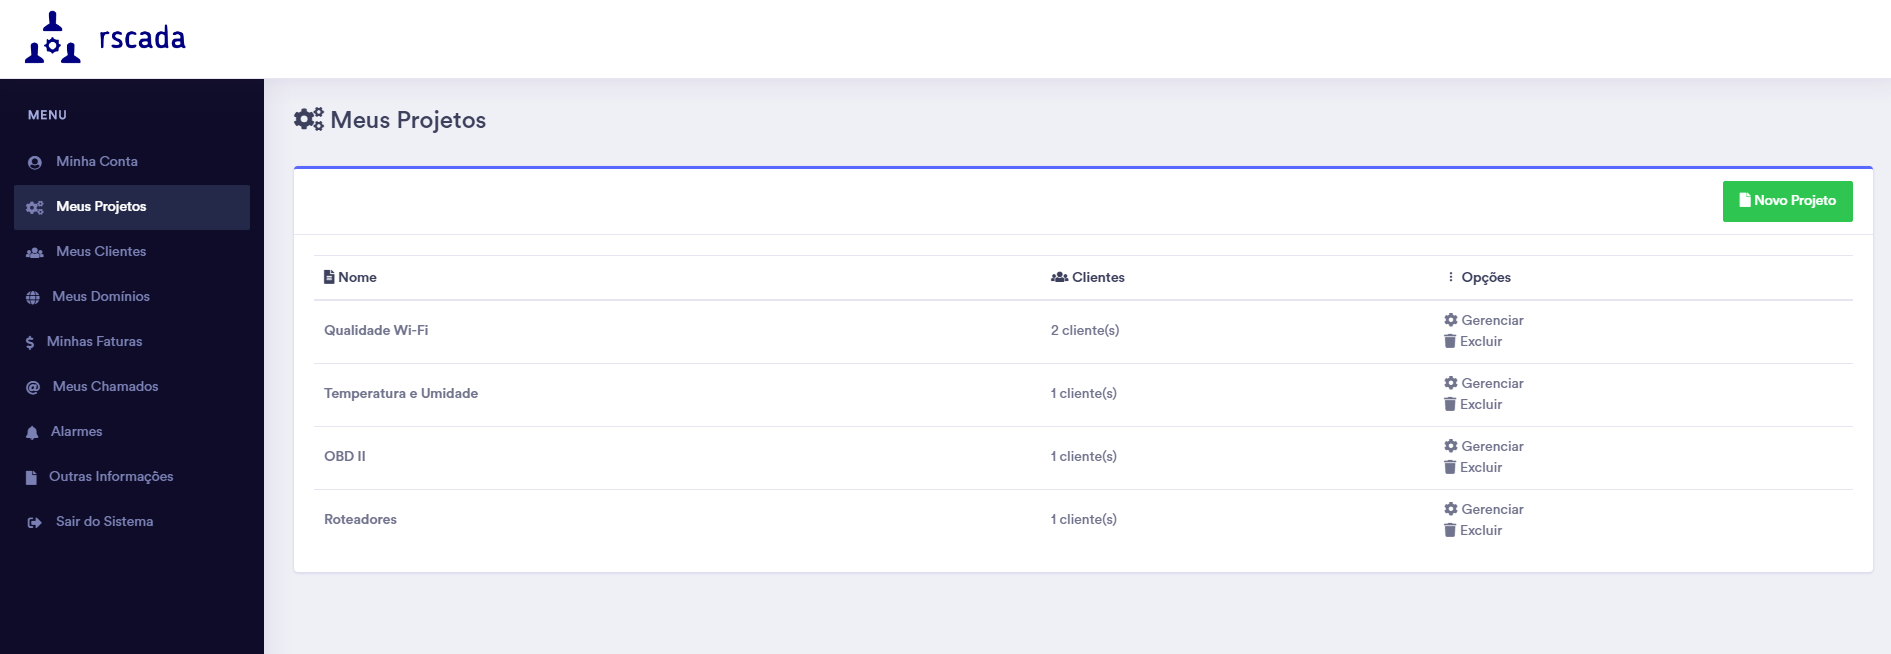
\includegraphics[width=15cm]{figuras/rscada-3.png}}
		}{
			\Fonte{O autor}
		}	
    	\end{figure}
    	
    	\begin{figure}[!h]
		\Caption{\label{fig:figura-rscada-5} Apresentação Geral de todos os projetos cadastrados.}
		%\centering
		\UFCfig{}{
			\fbox{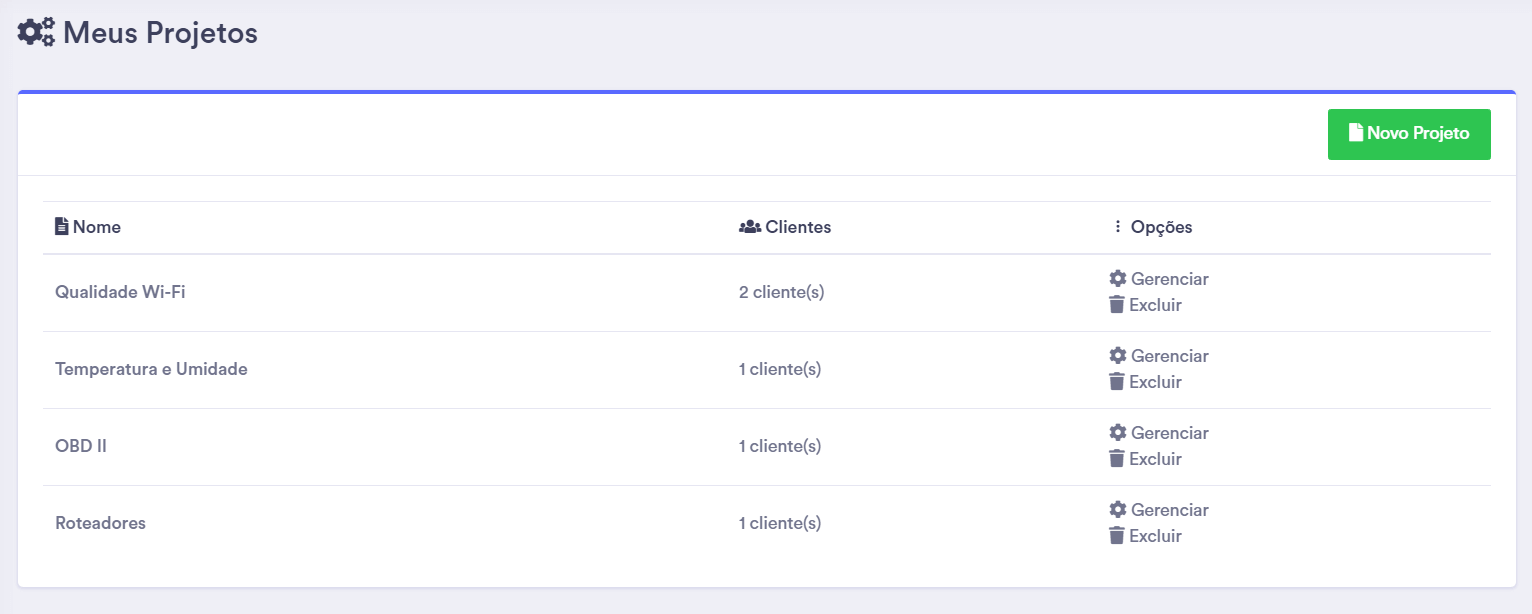
\includegraphics[width=15cm]{figuras/rscada-5.png}}
		}{
			\Fonte{O autor}
		}	
    	\end{figure}

A plataforma também permite o ajuste automático ao tipo de tela que o utilizador tenha, é a função que abre possibilidade para que o sistema seja adaptado à qualquer tipo de plataforma. Partindo do princípio que todo dispositivo conectado à internet tenha um navegador ou forma primitiva de um, é possível sua utilização, como exemplo, a Figura \ref{fig:figura-rscada-smartphone} traz uma captura de tela quando aberta em um \textit{smartphone}.

    	\begin{figure}[!h]
		\Caption{\label{fig:figura-rscada-smartphone} Tela inicial do sistema após autenticação em um \textit{smartphone}.}
		%\centering
		\UFCfig{}{
			\fbox{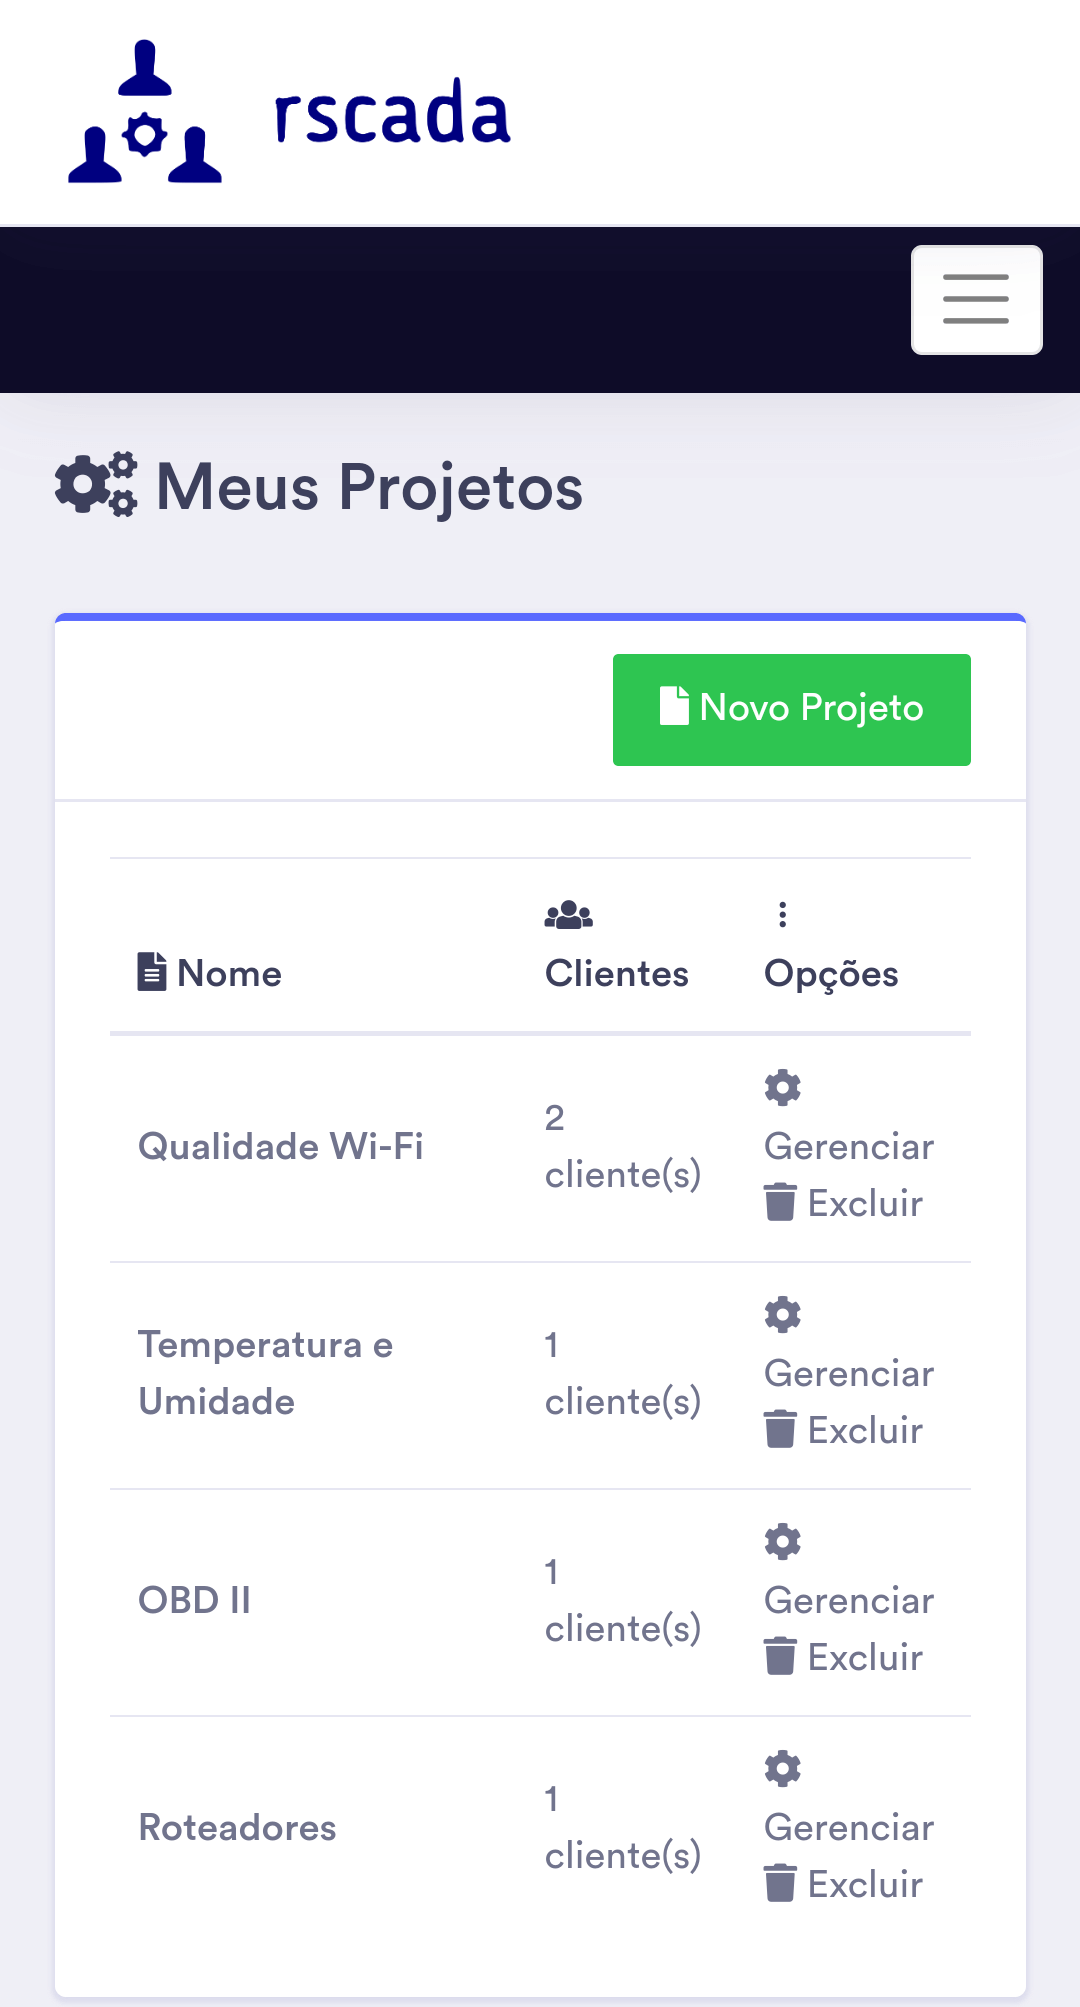
\includegraphics[width=6cm]{figuras/rscada-smartphone.png}}
		}{
			\Fonte{O autor}
		}	
    	\end{figure}
    	
\section{Criação de novos projetos}
\label{sec:criacao-projetos}
Ao clicar no botão Novo Projeto, o usuário é redirecionado à uma página solicitando o nome que se deseja para ele, conforme a Figura \ref{fig:figura-rscada-4}. Ao submeter o formulário é apresentada uma mensagem de sucesso, caso seja possível a criação dele e, em seguida, encaminhado à página inicial do projeto, representado na Figura \ref{fig:figura-rscada-novo}. 

        \begin{figure}[!h]
		\Caption{\label{fig:figura-rscada-4} Página de cadastro de novos Projetos.}
		%\centering
		\UFCfig{}{
			\fbox{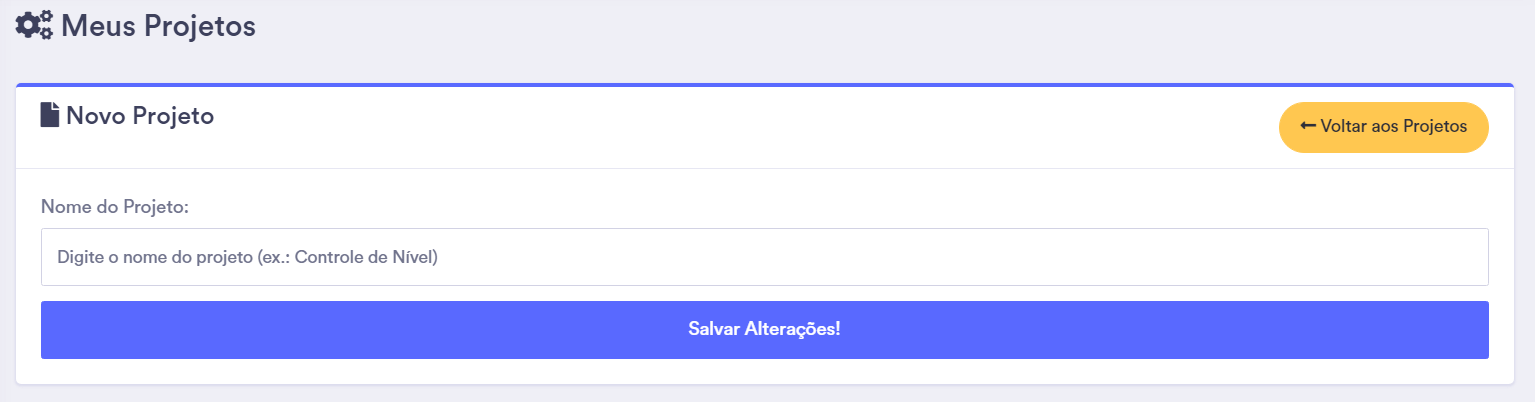
\includegraphics[width=15cm]{figuras/rscada-4.png}}
		}{
			\Fonte{O autor}
		}	
    	\end{figure}
    	
    	\begin{figure}[!h]
		\Caption{\label{fig:figura-rscada-novo} Página de gerenciamento de um novo projeto.}
		%\centering
		\UFCfig{}{
			\fbox{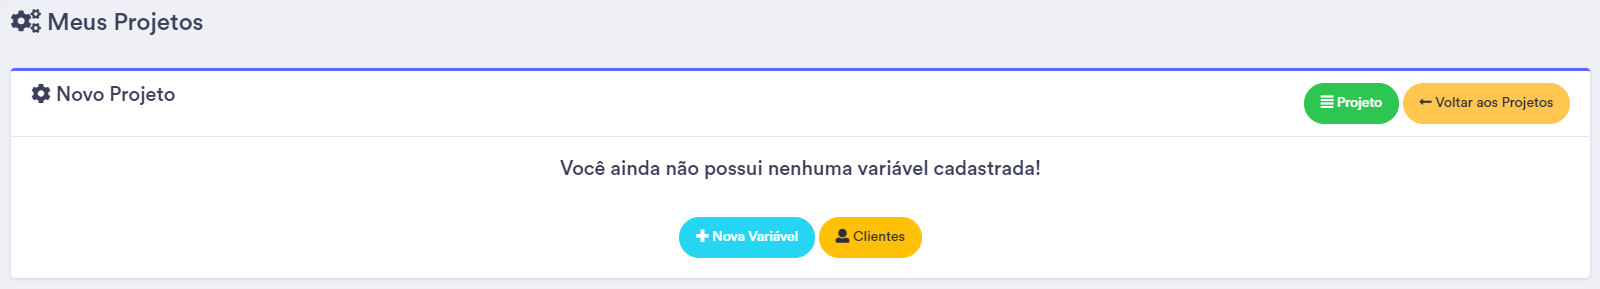
\includegraphics[width=15cm]{figuras/rscada-novo.png}}
		}{
			\Fonte{O autor}
		}	
    	\end{figure}

É apresentada uma mensagem de que não existe nenhuma variável cadastrada e há um reforço de cor no botão de criação para indicar a relevância dessa ação. Ao clicar no botão de Nova Variável, o usuário é redirecionado à uma tela ao qual poderá escolher o tipo pretendido, entre as citadas na seção \ref{sec:tipos-variaveis}, a variável iniciada por letra e minúscula, um nome que represente uma descrição à ela e a unidade correspondente caso exista. A Figura \ref{fig:figura-rscada-6} traz uma captura da tela de novas variáveis.

        \begin{figure}[!h]
		\Caption{\label{fig:figura-rscada-6} Página de cadastro de novas Variáveis.}
		%\centering
		\UFCfig{}{
			\fbox{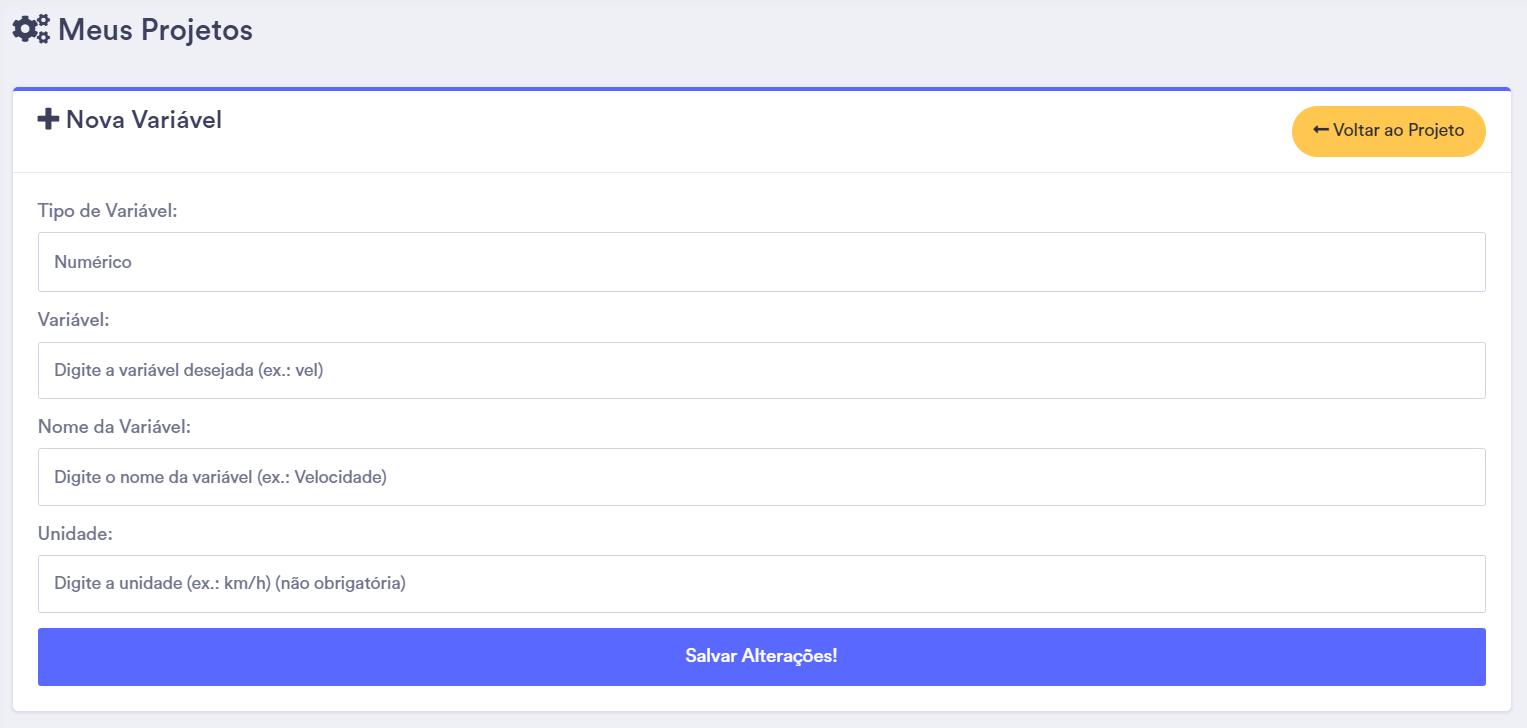
\includegraphics[width=15cm]{figuras/rscada-6.png}}
		}{
			\Fonte{O autor}
		}	
    	\end{figure}
    	
Quando submetido o formulário, é apresentada uma tela de sucesso caso a variável seja inserida no banco de dados e então, o usuário poderá gerenciar todas as variáveis já cadastradas no projeto com informação adicional sobre a quantidade de informações já inseridas no banco de dados para aquela variável específica, conforme representado na Figura \ref{fig:figura-rscada-variaveis} e coluna Registros. O cadastro de novas variáveis também pode ser feito diretamente no módulo de aquisição de dados, onde submetendo informações citando uma variável não cadastrada, o próprio módulo identificará o tipo dela e fará a submissão ao banco de dados. Este procedimento é feito para evitar a perda de informação, caso o desenvolvedor considere novas variáveis no dispositivo do processo e não tenha atualizado no sistema \gls{SCADA} ainda.

        \begin{figure}[!h]
		\Caption{\label{fig:figura-rscada-variaveis} Gerenciamento das variáveis cadastradas no projeto.}
		%\centering
		\UFCfig{}{
			\fbox{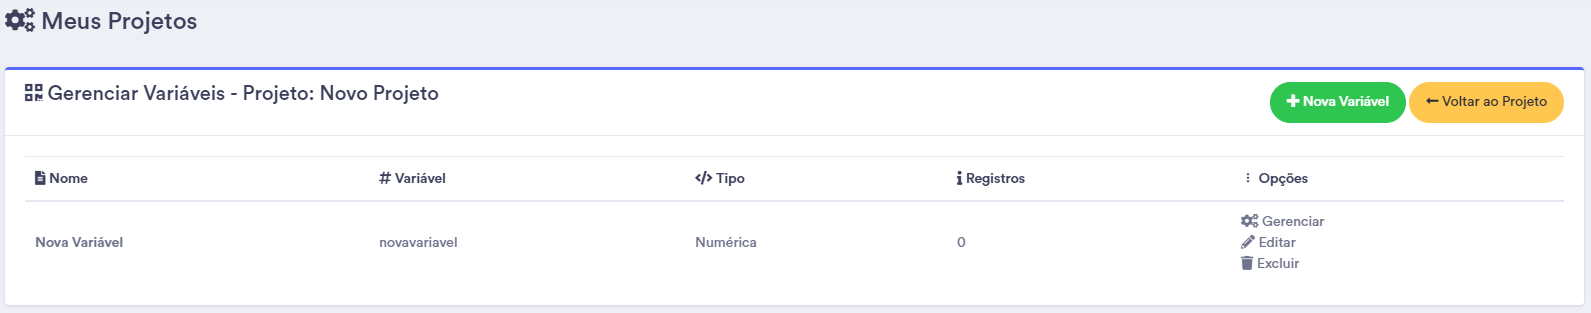
\includegraphics[width=15cm]{figuras/rscada-variaveis.png}}
		}{
			\Fonte{O autor}
		}	
    	\end{figure}

Com as variáveis já cadastradas no sistema, é oferecida a opção de criação de novos Objetos, detalhados na seção \ref{sec:projetos}, que quando clicado o botão, o usuário é direcionado à página ilustrada pela Figura \ref{fig:figura-rscada-7}. São solicitados o tipo do objeto, entre as opções já disponíveis na data de apresentação deste trabalho os seguintes:

\begin{alineascomponto}
    \item Chave Binária: disponibiliza um botão que controla uma variável binária, à qual cada clique inverte seu valor, foi desenvolvida pensando em ser utilizada na função liga/desliga de alguma ação dentro do processo que seja necessário.
    \item Botão de Ação: disponibiliza um botão que pode oferecer o envio de um valor determinado em uma variável no instante em que for solicitado, foi desenvolvido pensando em ser utilizado em funções que não sejam sustentadas, ou seja, tenha um único acionamento com período de duração determinado.
    \item Último Valor: disponibiliza um texto fixo com o último valor enviado pelo dispositivo da variável desejada no objeto, é dada a variação em relação ao valor imediatamente anterior à ele e o tempo que se passou desde o último envio.
    \item Gráfico de Linha: disponibiliza na tela um gráfico de linhas com uma série temporal das informações enviadas à variável escolhida. 
    \item Gráfico de Área: disponibiliza na tela um gráfico de área com uma série temporal das informações enviadas à variável escolhida.
    \item Gráfico de Barras: disponibiliza na tela um gráfico de barras com uma série temporal das informações enviadas à variável escolhida.
    \item Tabela de Informações: disponibiliza na tela uma tabela contendo uma quantidade dos últimos valores das informações enviadas à variável escolhida.
    \item Tabela de Eventos:  disponibiliza na tela uma tabela contendo os registros de alarmes e alertas sobre envio de informações que não estejam em acordo com o definido para a variável escolhida, representando também os alertas visuais que serão oferecidos ao operador quando ocorridas. A Figura \ref{fig:figura-rscada-alarmes} traz exemplos dos alarmes que são emitidos em tela para o Operador.
\end{alineascomponto}

Em seguida, são solicitados: Título, Descrição e Tamanho do Objeto, que servirão para apresentação da caixa gráfica quando inserida na interface do projeto. O Tamanho é uma seleção entre: Pequeno, Médio, Grande e Gigante, sendo respectivamente relacionado à largura ocupada da tela pelo Objeto, 25\%, 50\%, 75\% e 100\%.

        \begin{figure}[!h]
		\Caption{\label{fig:figura-rscada-7} Página de cadastro de novos Objetos.}
		%\centering
		\UFCfig{}{
			\fbox{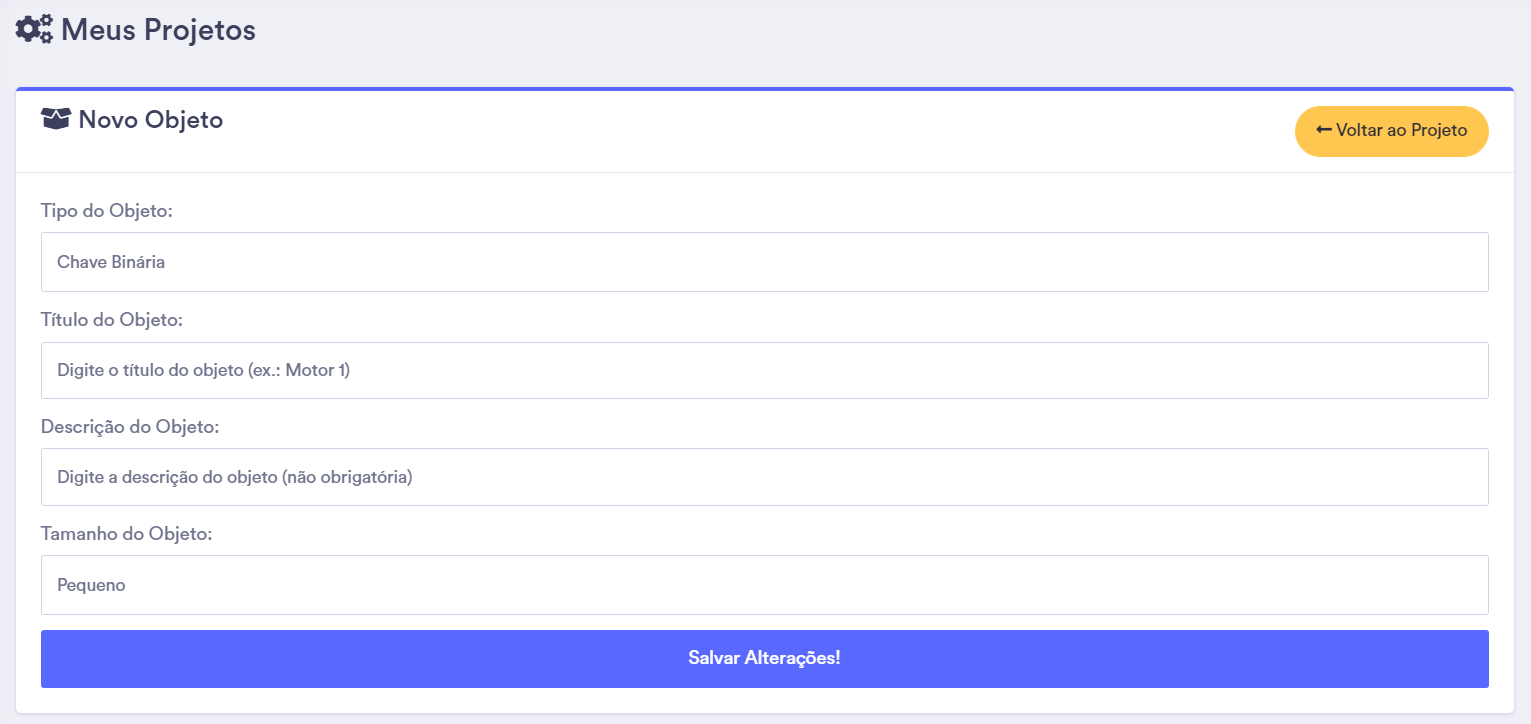
\includegraphics[width=15cm]{figuras/rscada-7.png}}
		}{
			\Fonte{O autor}
		}	
    	\end{figure}
    	
    	\begin{figure}[!h]
		\Caption{\label{fig:figura-rscada-alarmes} Alertas do sistema quando há uma não-conformidade da informação recebida.}
		%\centering
		\UFCfig{}{
			\fbox{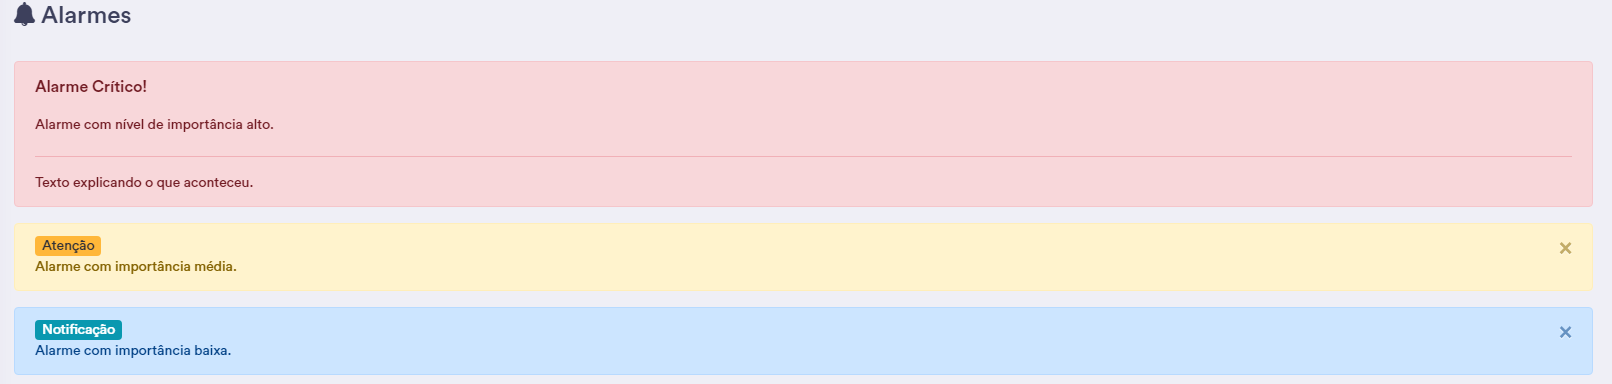
\includegraphics[width=15cm]{figuras/rscada-alarmes.png}}
		}{
			\Fonte{O autor}
		}	
    	\end{figure}
    	
Quando criado o objeto, é solicitada a edição dele para a determinação dos parâmetros referentes ao tipo específico escolhido, conforme a Figura \ref{fig:figura-rscada-10}.
        
        \begin{figure}[!h]
		\Caption{\label{fig:figura-rscada-10} Objeto recém-criado.}
		%\centering
		\UFCfig{}{
			\fbox{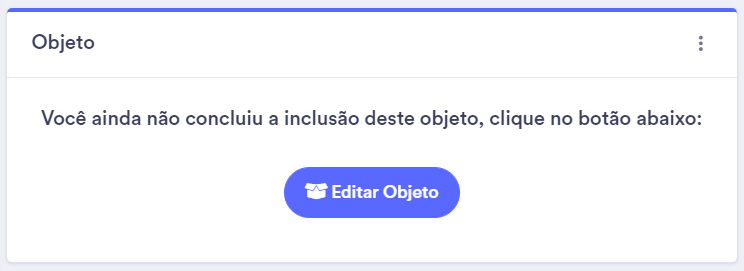
\includegraphics[width=10cm]{figuras/rscada-10.png}}
		}{
			\Fonte{O autor}
		}	
    	\end{figure}
    	
Na tela referente à edição do Objeto, é selecionada a variável que o objeto manipulará e a Janela de Tempo que seria a quantidade de pontos de informação à serem consideradas pelo sistema quando gerar o Objeto na interface de gerenciamento. A Figura \ref{fig:figura-rscada-editar-objeto} traz um exemplo de edição de um objeto do tipo Tabela de Informações em uma Nova Variável e Janela de Tempo de 5 minutos.

    	
    	\begin{figure}[!h]
		\Caption{\label{fig:figura-rscada-editar-objeto} Edição de objeto para determinação de parâmetros.}
		%\centering
		\UFCfig{}{
			\fbox{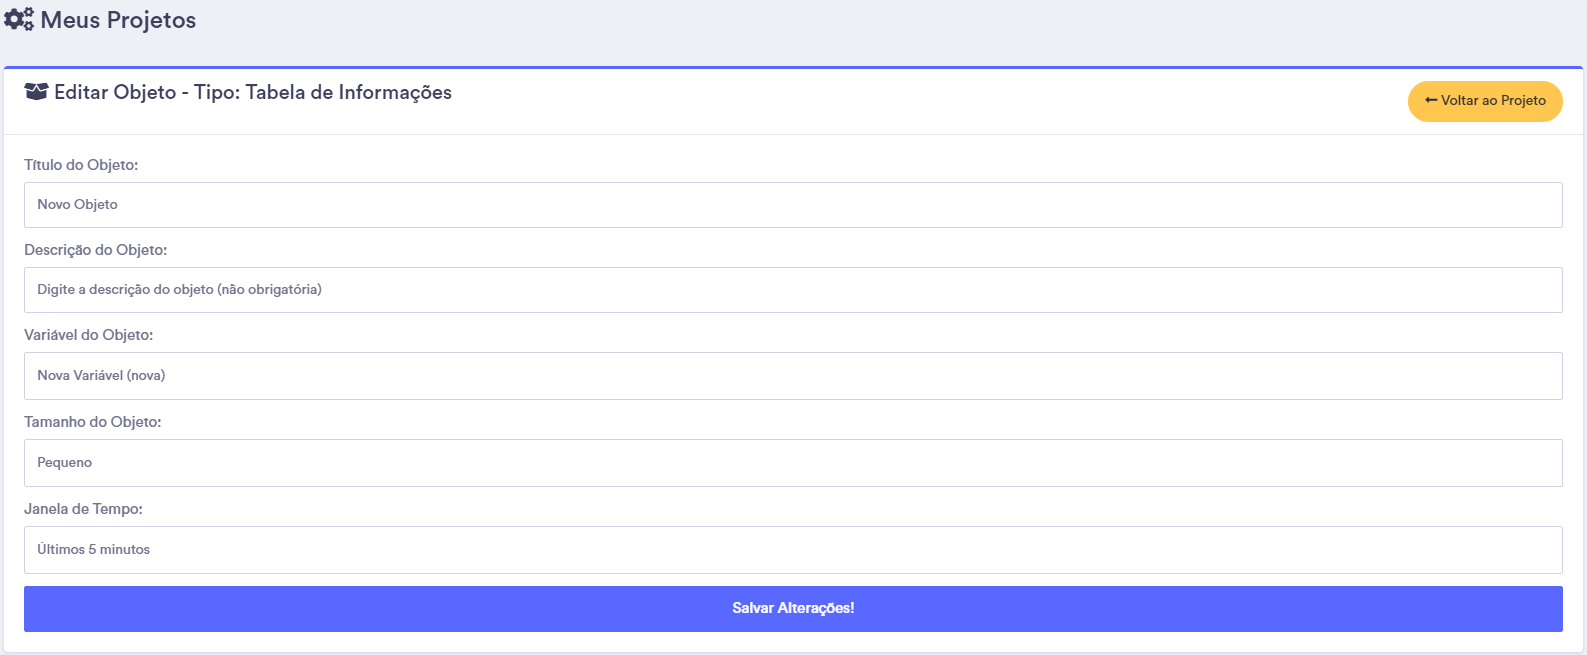
\includegraphics[width=15cm]{figuras/rscada-editar-objeto.png}}
		}{
			\Fonte{O autor}
		}	
    	\end{figure}

Após a organização dos Objetos e Variáveis das etapas acima, deve ser feita a inclusão no menu Meus Clientes, dos operadores que utilizarão o projeto criado. A página Meus Clientes, disponibiliza um botão Novo Cliente, que após clicado, solicita dados do cliente, como: Nome, E-mail, Usuário e Senha que servirão para acesso do mesmo à interface de gerenciamento quando incluso no projeto. A Figura \ref{fig:figura-rscada-novo-cliente} traz a página de inclusão de novos clientes.

        \begin{figure}[!h]
		\Caption{\label{fig:figura-rscada-novo-cliente} Inserção de novo cliente ao sistema.}
		%\centering
		\UFCfig{}{
			\fbox{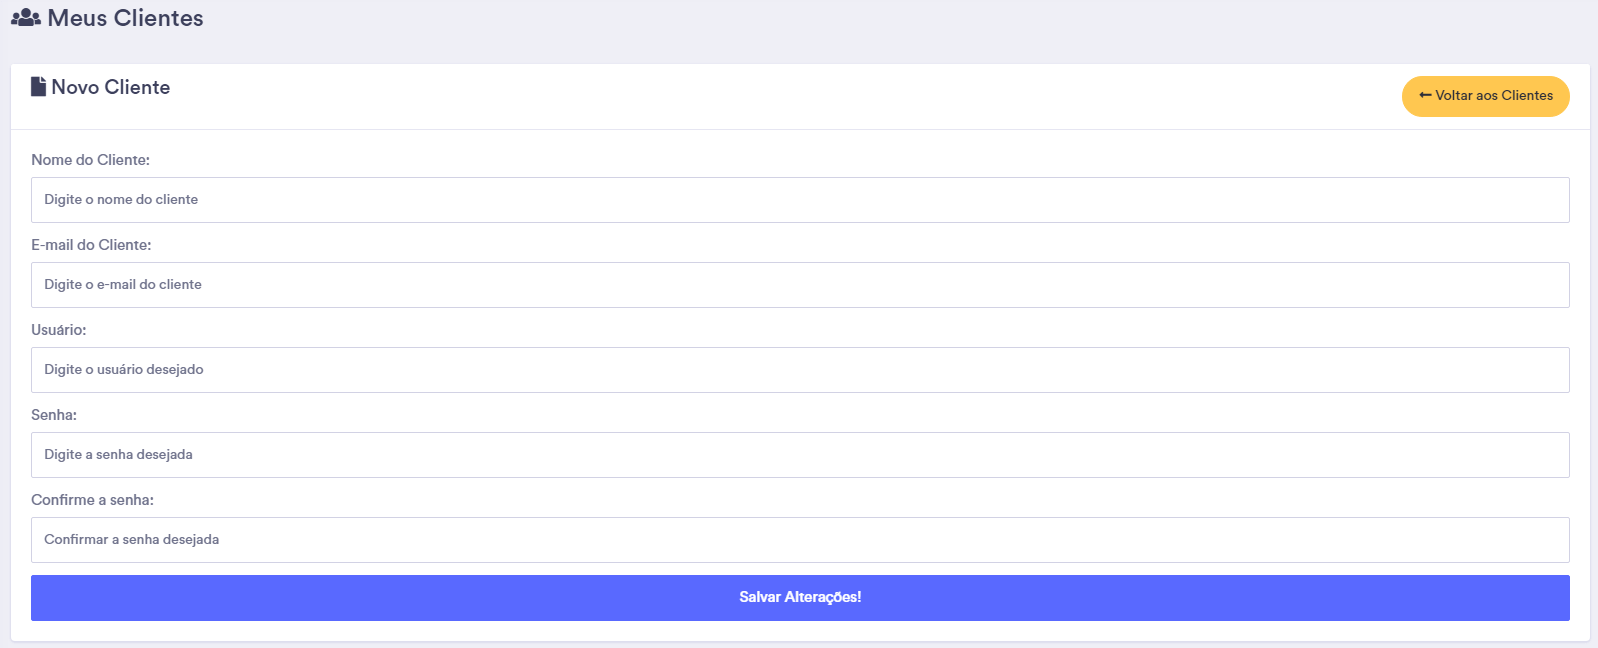
\includegraphics[width=15cm]{figuras/rscada-novo-cliente.png}}
		}{
			\Fonte{O autor}
		}	
    	\end{figure}
    	
A submissão do formulário com os dados do cliente, desde que corretamente inseridos no banco de dados, resultará numa página com uma mensagem de sucesso e o usuário será direcionado à tela de gerenciamento de todos os clientes cadastrados no sistema, outras ações são disponíveis também nesta seção como o gerenciamento do cliente, alteração de seus dados de cadastro e a exclusão do mesmo, conforme a Figura \ref{fig:figura-rscada-clientes}.
    	
    	\begin{figure}[!h]
		\Caption{\label{fig:figura-rscada-clientes} Gerenciamento dos clientes cadastrados no sistema.}
		%\centering
		\UFCfig{}{
			\fbox{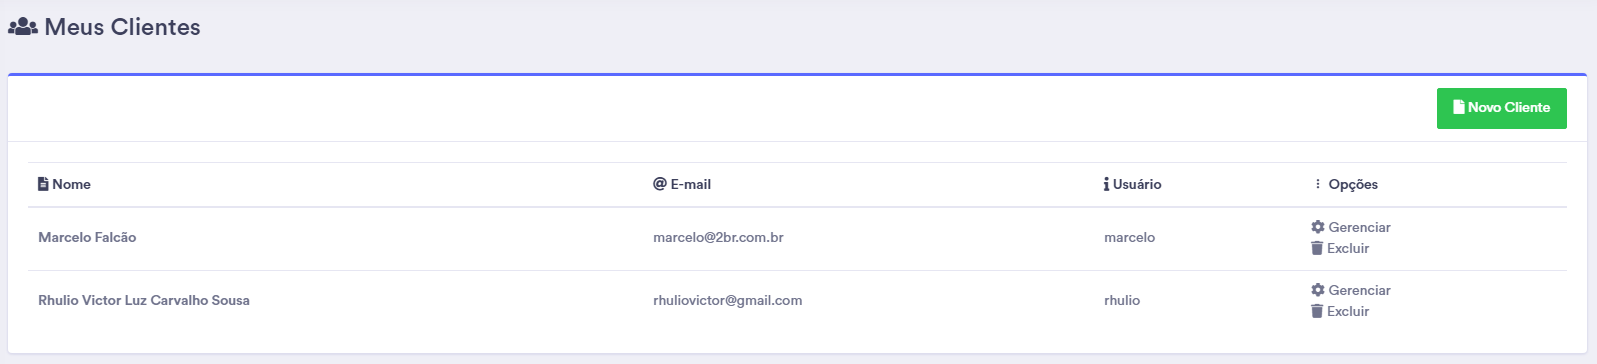
\includegraphics[width=15cm]{figuras/rscada-clientes.png}}
		}{
			\Fonte{O autor}
		}	
    	\end{figure}
    	
Após inserido um novo cliente, é possível fazer a associação do mesmo ao projeto criado anteriormente. A Figura \ref{fig:figura-rscada-8} traz detalhes de como é realizada esta ação no sistema.
    	
        \begin{figure}[!h]
		\Caption{\label{fig:figura-rscada-8} Associação de novo cliente ao projeto.}
		%\centering
		\UFCfig{}{
			\fbox{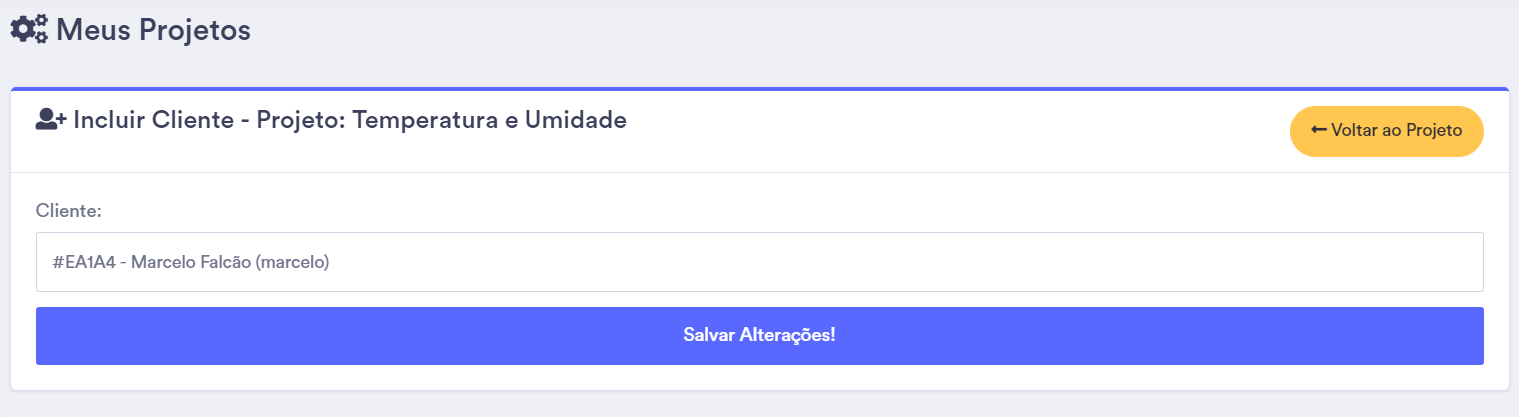
\includegraphics[width=15cm]{figuras/rscada-8.png}}
		}{
			\Fonte{O autor}
		}	
    	\end{figure}

Desde que seja corretamente associado o cliente ao projeto e inserida esta informação no banco de dados, é retornada uma página de sucesso e o usuário é redirecionado à página de Clientes Associados, onde podem ser verificados o \textit{Token} de acesso para envio de informações, nível do cliente e quantidade de informações enviadas por ele. Estão disponíveis também outras ferramentas, como: Editar a associação entre cliente e projeto e, a exclusão do mesmo, conforme a Figura \ref{fig:figura-rscada-9} que traz detalhes da tela.

        \begin{figure}[!h]
		\Caption{\label{fig:figura-rscada-9} Visão geral dos clientes cadastrados no projeto.}
		%\centering
		\UFCfig{}{
			\fbox{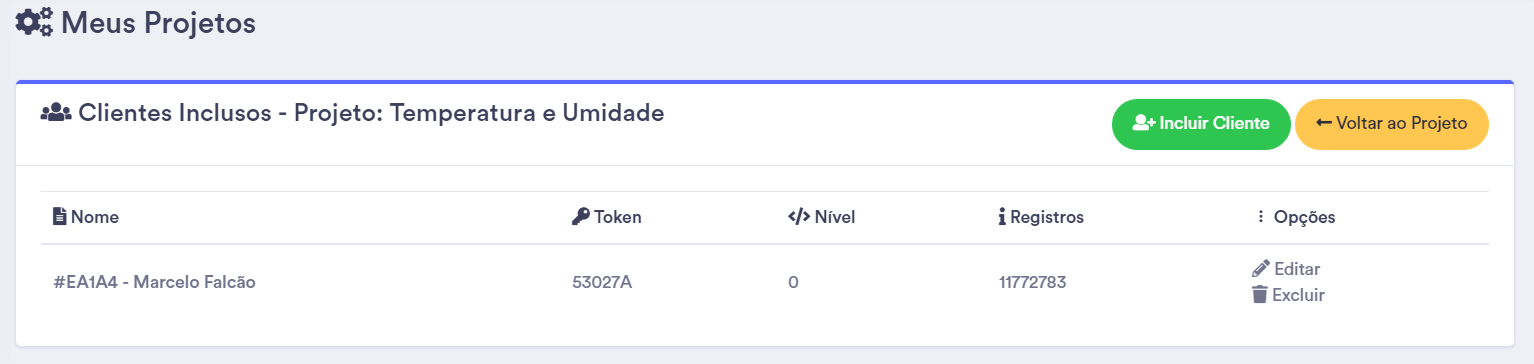
\includegraphics[width=15cm]{figuras/rscada-9.png}}
		}{
			\Fonte{O autor}
		}	
    	\end{figure}
    	
\section{Síntese}
\label{sec:sintese-rscada}

A abordagem utilizada neste Capítulo, pode ser sintetizada por um Diagrama de Caso de Uso, descrevendo a sequência e as unidades de interação com o sistema, disponível na Figura \ref{fig:figura-diagrama-uso}. Tendo sido detalhadas todas as funcionalidades propostas desenvolvidas, o capítulo seguinte traz uma aproximação do uso real deste sistema, com base em exemplos de diversas situações de utilização do mesmo. Os dois protocolos de aquisição de dados, \gls{MQTT} e \gls{HTTP}, são utilizados para demonstrar a facilidade de uso e a capacidade de integração do sistema.

        \begin{figure}[!h]
		\Caption{\label{fig:figura-diagrama-uso} Diagrama de caso de uso sintetizando os níveis de permissão do sistema.}
		%\centering
		\UFCfig{}{
			\fbox{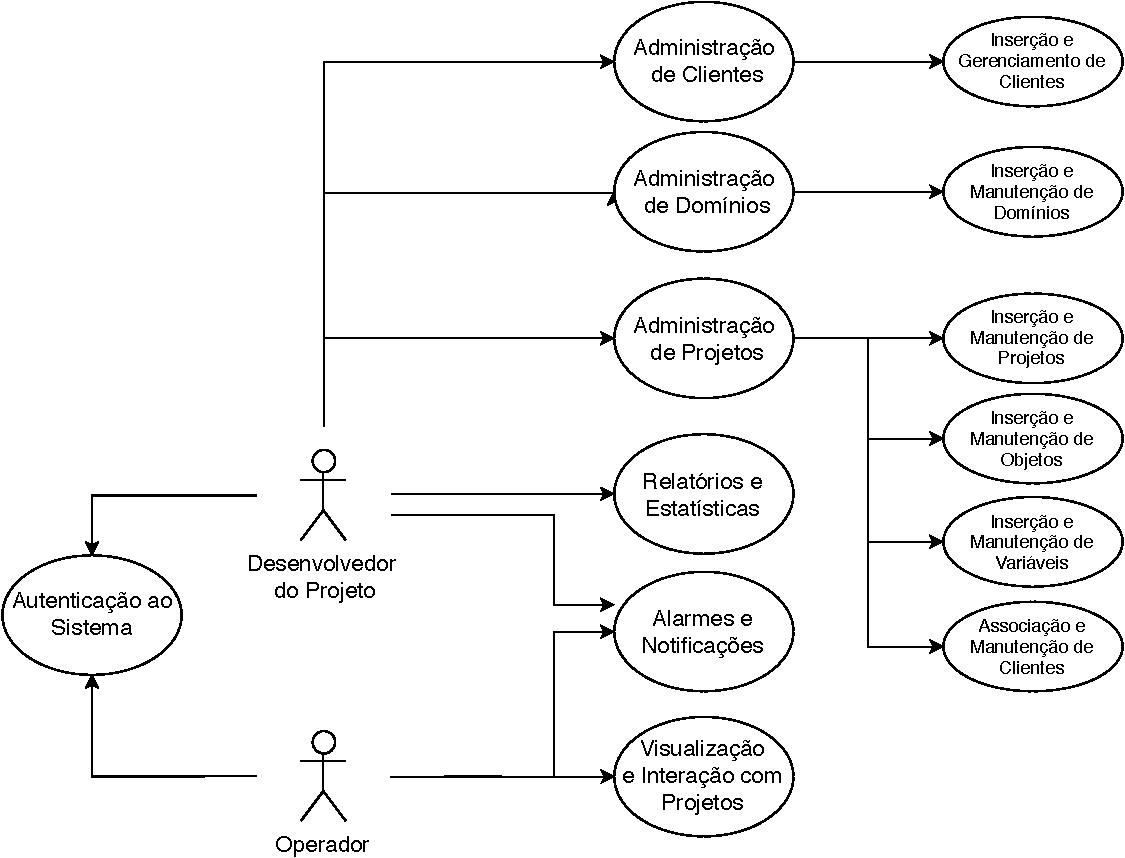
\includegraphics[width=15cm]{figuras/figura-diagrama-uso.pdf}}
		}{
			\Fonte{O autor}
		}	
    	\end{figure}
    	
	\chapter{Resultados}
\label{chap:resultados}

Para exemplificação do uso do sistema proposto na prática, foram desenvolvidos alguns projetos de exemplo. Devido a dificuldade na implementação de uma planta completa com dispositivos normalmente encontrados na Indústria, foram utilizados microcontroladores para gerar as informações disponíveis nas seções abaixo que trarão os mesmos efeitos caso fossem utilizados dispositivos industriais com conexão à \textit{internet}.

\section{Temperatura e Umidade}
\label{sec:temperatura-umidade}

Este exemplo tem por objetivo a utilização de variáveis de ambiente em simulação de um processo industrial que fosse necessário o acompanhamento de informações de temperatura e umidade. Foram utilizados os seguintes materiais: (i) Placa de desenvolvimento com microcontrolador ESP8266 da fabricante \textit{espressif}, visto na Figura \ref{fig:figura-nodemcu} e (ii) Módulo com sensor de temperatura e umidade DHT11 da fabricante chinesa \textit{Aosong Electronics Co. Ltd}, visto na Figura \ref{fig:figura-dht11}.

O código para este exemplo, anexo \ref{an:anexo-temperatura-umidade}, foi desenvolvido através da linguagem de programação C++ adaptada ao \textit{Arduino} e os dados são transmitidos ao rscada utilizando o protocolo \gls{MQTT}, devido ser a forma de comunicação mais leve para um pequeno dispositivo como o microcontrolador utilizado.

        \begin{figure}[!h]
		\Caption{\label{fig:figura-nodemcu} Placa de desenvolvimento com microcontrolador ESP8266 da fabricante \textit{espressif}.}
		%\centering
		\UFCfig{}{
			\fbox{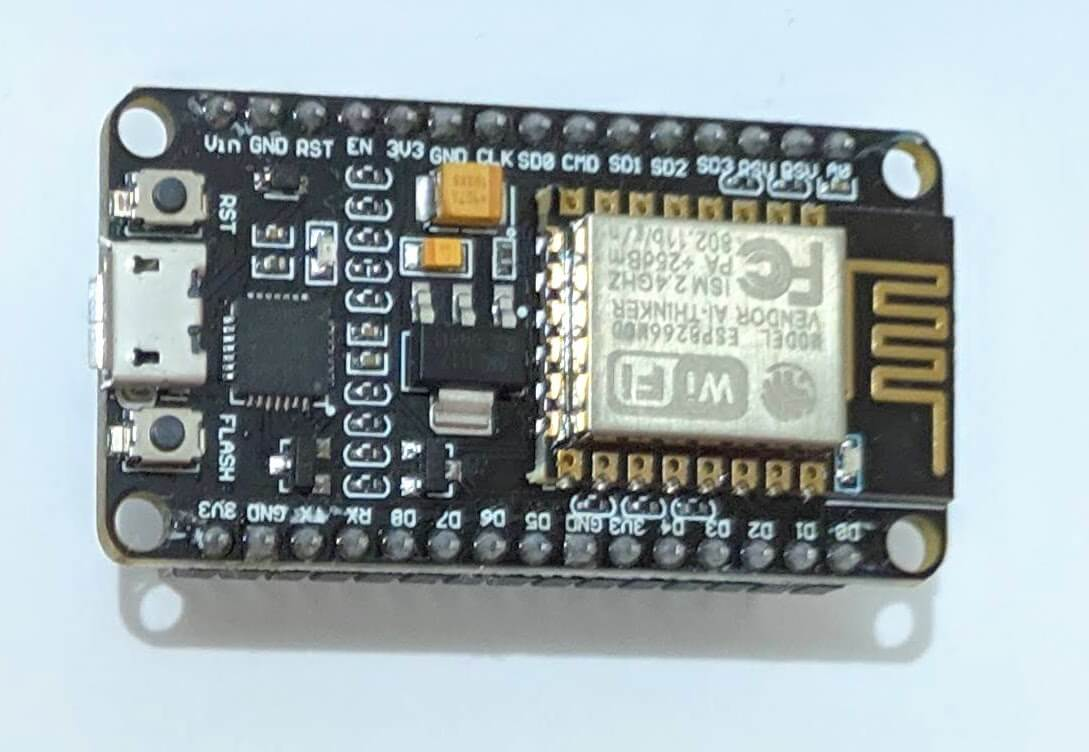
\includegraphics[width=5cm]{figuras/nodemcu.jpg}}
		}{
			\Fonte{O autor}
		}	
    	\end{figure}
    	
    	\begin{figure}[!h]
		\Caption{\label{fig:figura-dht11} Módulo com sensor de temperatura e umidade DHT11.}
		%\centering
		\UFCfig{}{
			\fbox{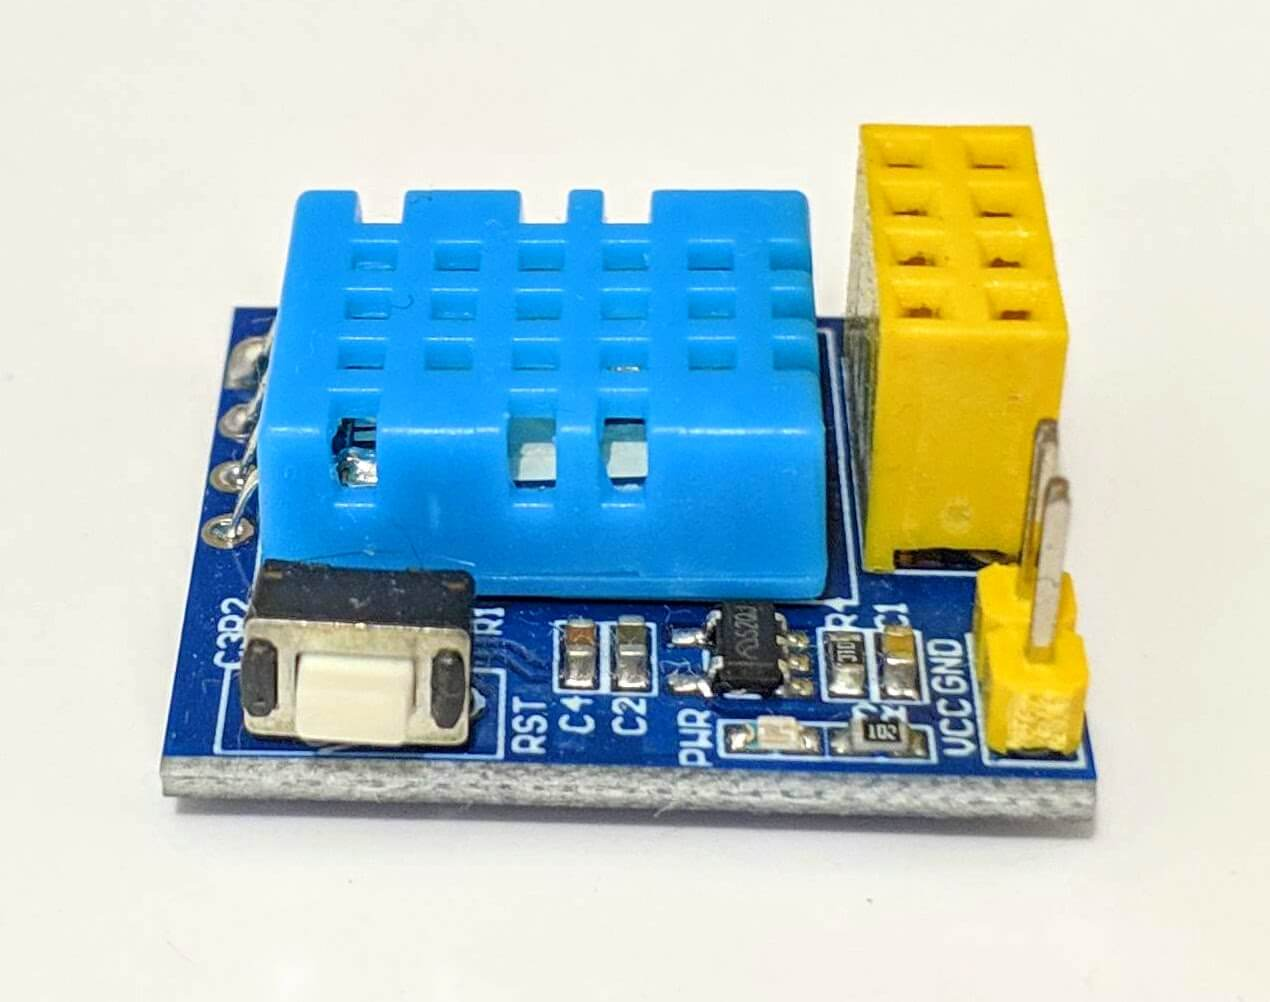
\includegraphics[width=5cm]{figuras/modulo-dht11.jpg}}
		}{
			\Fonte{O autor}
		}	
		
    	\end{figure}
    	
Inicialmente foram configuradas as variáveis à serem utilizadas pelo programa do microcontrolador, sendo elas: (i) Latência, representando o tempo de atraso entre o envio da informação e a resposta do servidor, (ii) Temperatura e (iii) Umidade, ambas do tipo numérica já que representarão números inteiros ou irracionais. A Figura \ref{fig:figura-temperatura-variaveis} traz uma captura da tela de gerenciamento de variáveis, com o exemplo já em funcionamento e um histórico com mais de 4 milhões de pontos de informação em cada variável.

        \begin{figure}[!h]
		\Caption{\label{fig:figura-temperatura-variaveis} Variáveis utilizadas para o projeto.}
		%\centering
		\UFCfig{}{
			\fbox{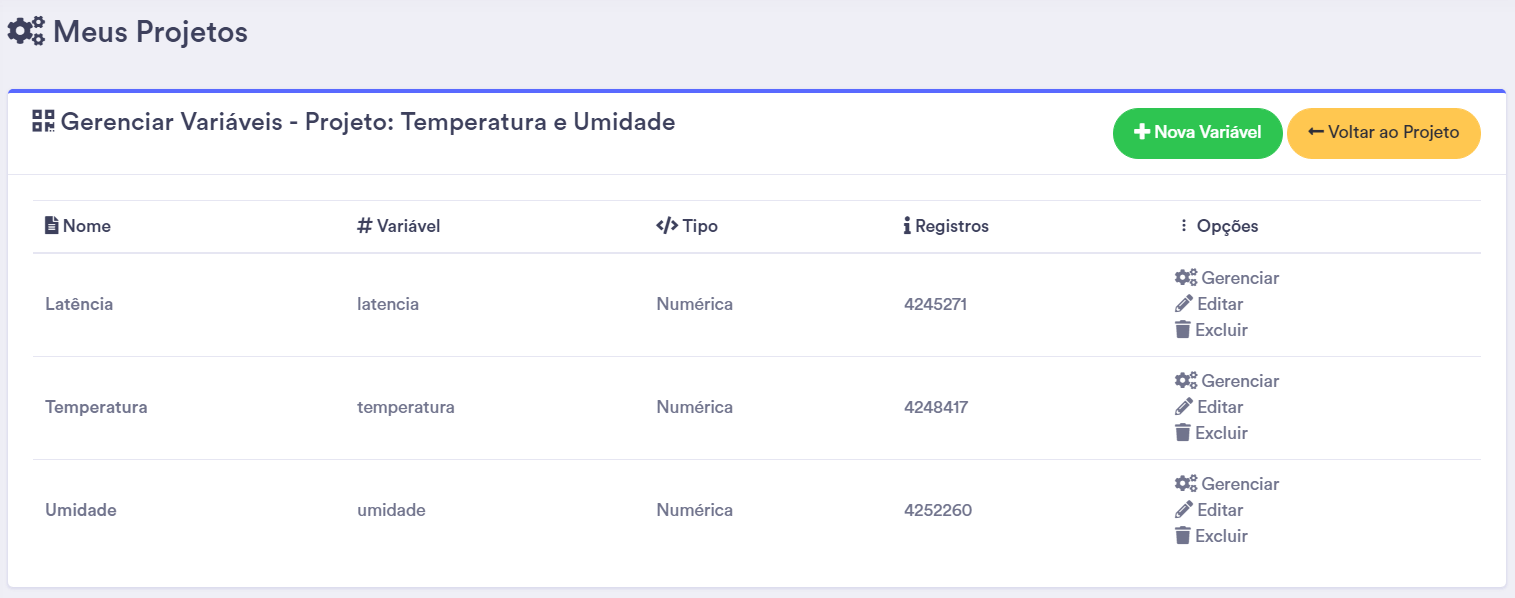
\includegraphics[width=15cm]{figuras/temperatura-variaveis.png}}
		}{
			\Fonte{O autor}
		}	
    	\end{figure}
    	
Para este exemplo foram utilizados um total de 6 objetos, sendo os 3 primeiros do tipo Últimor Valor para demonstrar os valores instantâneos recebidos pelo microcontrolador e suas variações, representados na Figura \ref{fig:figura-temperatura-instataneos} e outros 3 do tipo gráfico, para acompanhar a variação das informações através do tempo em uma janela de tempo configurada com 30 minutos de período. As Figuras \ref{fig:figura-temperatura-grafico} e  \ref{fig:figura-temperatura-umidade} representam os objetos: temperatura e umidade, do tipo Gráfico de Área e a Figura \ref{fig:figura-temperatura-latencia}, a latência da conexão, do tipo Gráfico de Linha.

        \begin{figure}[!h]
		\Caption{\label{fig:figura-temperatura-instataneos} Últimas informações enviadas.}
		%\centering
		\UFCfig{}{
			\fbox{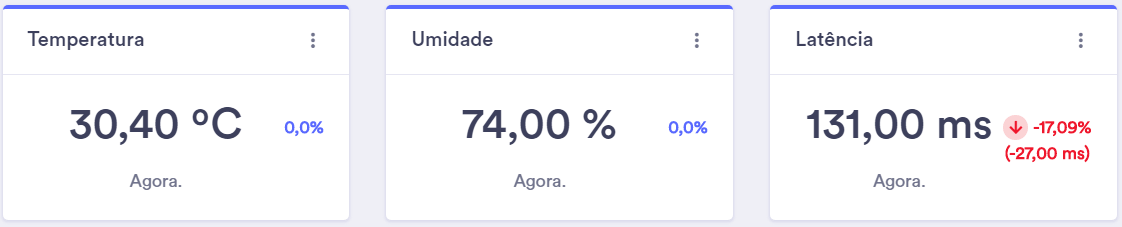
\includegraphics[width=15cm]{figuras/temperatura-instataneos.png}}
		}{
			\Fonte{O autor}
		}	
    	\end{figure}
    	
Os objetos do tipo Último Valor, na Figura \ref{fig:figura-temperatura-instataneos}, foram utilizados para representar os valores instantâneos das variáveis principais do processo, neles, são disponibilizadas as informações sobre há quanto tempo foi enviado o último dado e qual sua variação, em ambos os casos ocorre um alerta caso a temperatura ultrapasse um valor pré-definido ou não tenha a inserção de novos dados durante um dado tempo.

        \begin{figure}[!h]
		\Caption{\label{fig:figura-temperatura-grafico} Gráfico de área com os últimos 30 minutos de temperatura registrada.}
		%\centering
		\UFCfig{}{
			\fbox{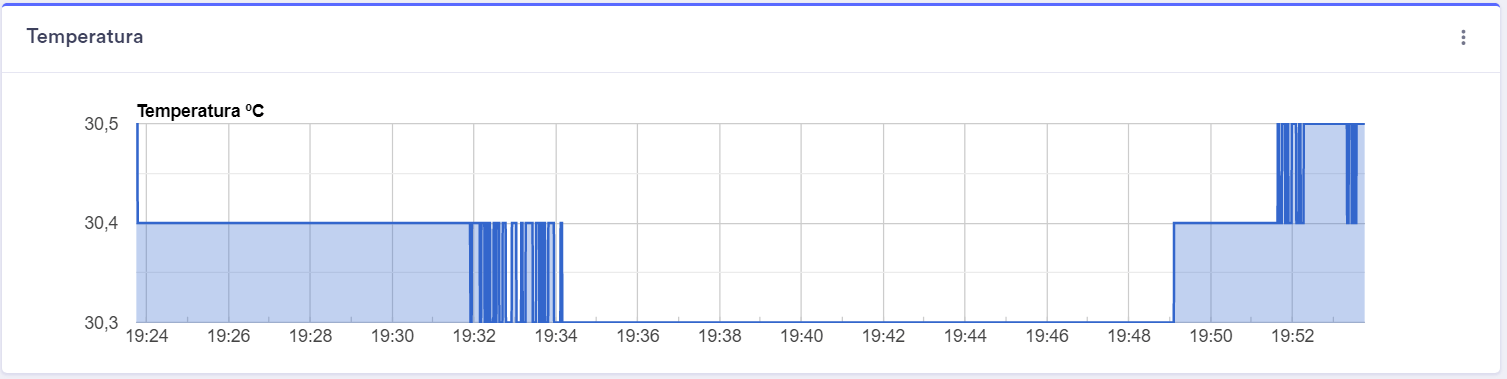
\includegraphics[width=15cm]{figuras/temperatura-grafico.png}}
		}{
			\Fonte{O autor}
		}	
    	\end{figure}
    	
Para o período de captura utilizado neste exemplo, Figura \ref{fig:figura-temperatura-grafico}, houve um intervalo de temperatura entre 30,3 e 30,5ºC, onde a precisão da medição do modelo de sensor utilizado é na casa de 0,1ºC. Devido um parâmetro configurado no gráfico, as amplitudes de temperatura não são demonstradas desde o ponto zero, mas sim, somente entre a temperatura mínima e a máxima, tornando fácil a identificação destes extremos na janela de tempo escolhida. O Gráfico de umidade, representado na Figura \ref{fig:figura-temperatura-umidade}, foi parametrizado seguindo as mesmas observações feitas anteriormente, revelando uma oscilação no mesmo período de tempo da figura anterior, entre 71 e 74\% de umidade relativa do ar com uma precisão do sensor na casa de 1\%.

        \begin{figure}[!h]
		\Caption{\label{fig:figura-temperatura-umidade} Gráfico de área com os últimos 30 minutos de umidade registrada.}
		%\centering
		\UFCfig{}{
			\fbox{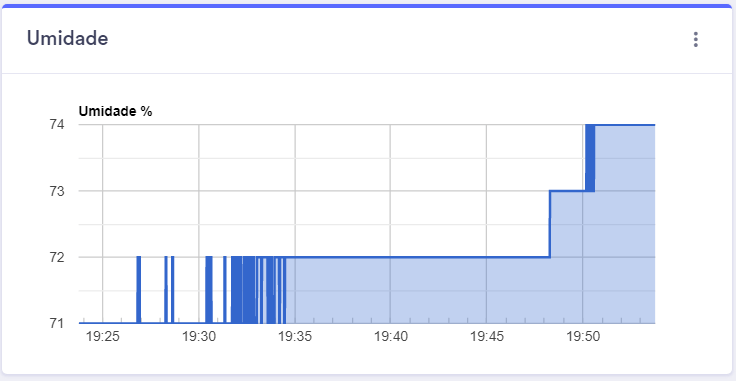
\includegraphics[width=8cm]{figuras/temperatura-umidade.png}}
		}{
			\Fonte{O autor}
		}	
    	\end{figure}
    	
O acompanhamento da latência da conexão entre o microcontrolador e o servidor também foi feito, para que possíveis erros de medição ou atrasos, fossem facilmente identificados. Na Figura \ref{fig:figura-temperatura-latencia}, é possível perceber um leve aumento na latência entre 19h52 e 19h54 do dia em que a captura foi feita, provavelmente devido ao pico de demanda do provedor neste horário.
    	
        \begin{figure}[!h]
		\Caption{\label{fig:figura-temperatura-latencia} Gráfico de linhas com os últimos 30 minutos de latência registrada.}
		%\centering
		\UFCfig{}{
			\fbox{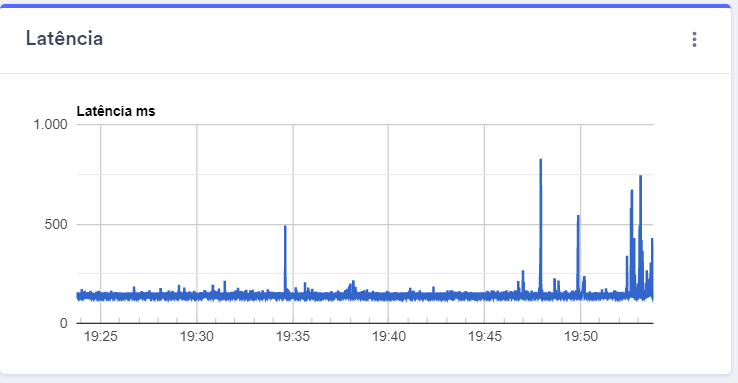
\includegraphics[width=8cm]{figuras/temperatura-latencia.png}}
		}{
			\Fonte{O autor}
		}	
    	\end{figure}
\section{Qualidade Sinal - WiFi}
\label{sec:qualidade-sinal}

O objetivo deste segundo exemplo é acompanhar os níveis de qualidade de sinal, como: potência do sinal recebido e latência da conexão de uma rede  \textit{Wi-Fi} doméstica e um teste com o botão liga/desliga para o controle do status do monitoramento. Para este projeto foi utilizada uma placa de desenvolvimento com microcontrolador ESP32 da fabricante \textit{espressif}, vista na Figura \ref{fig:figura-esp32}, que já possui integrado de fábrica o modem \textit{Wi-Fi}.

O código para este exemplo, anexo \ref{an:anexo-wifi}, também foi desenvolvido através da linguagem de programação C++ adaptada ao \textit{Arduino} e os dados são transmitidos ao rscada utilizando o protocolo \gls{MQTT}, assim como o exemplo anterior, devido ser a forma de comunicação mais leve para um pequeno dispositivo como o microcontrolador utilizado.

        \begin{figure}[!h]
		\Caption{\label{fig:figura-esp32} Placa de desenvolvimento com microcontrolador ESP32 da fabricante \textit{espressif}.}
		%\centering
		\UFCfig{}{
			\fbox{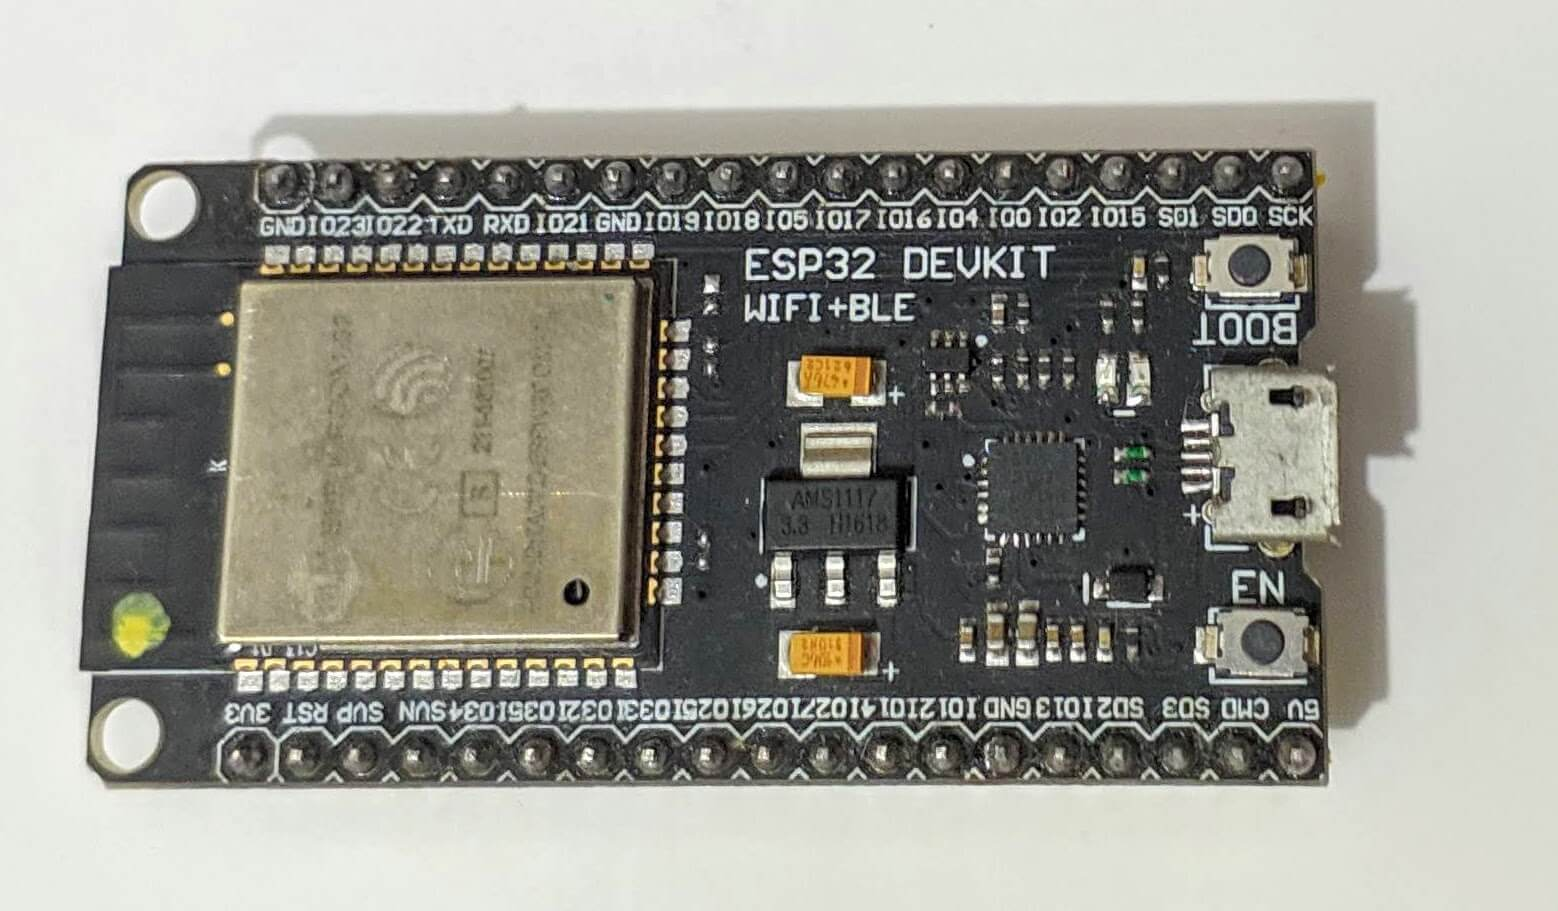
\includegraphics[width=5cm]{figuras/esp32.jpg}}
		}{
			\Fonte{O autor}
		}	
    	\end{figure}
    	
Inicialmente foram configuradas as variáveis à serem utilizadas pelo programa do microcontrolador, sendo elas: (i) Monitoramento, uma variável do tipo binária para o controle da chave liga/desliga, (ii)  Latência, representando o tempo de atraso entre o envio da informação e a resposta do servidor e (iii) Nível de Sinal, ambas do tipo numérica já que representarão números inteiros ou irracionais. A Figura \ref{fig:figura-wifi-variaveis} traz uma captura da tela de gerenciamento de variáveis, com o exemplo já em funcionamento e um histórico com mais de 4 milhões de pontos de informação em uma das variáveis do tipo numérica, a variável binária não possui registro de informações devido ser considerado como  \textit{booleana} apenas.

        \begin{figure}[!h]
		\Caption{\label{fig:figura-wifi-variaveis} Variáveis utilizadas no projeto.}
		%\centering
		\UFCfig{}{
			\fbox{\includegraphics[width=15cm]{figuras/wifi-variaveis.png}}
		}{
			\Fonte{O autor}
		}	
    	\end{figure}


Foram utilizados um total de 5 objetos, sendo o primeiro, uma chave para ligar ou desligar o monitoramento do exemplo, duas do tipo Último Valor para demonstrar os valores instantâneos recebidos pelo microcontrolador e suas variações, representados na Figura \ref{fig:figura-wifi-instataneos} e outros 2 do tipo gráfico, para acompanhar a variação das informações através do tempo em uma janela de tempo configurada com 10 minutos de período. 

        \begin{figure}[!h]
		\Caption{\label{fig:figura-wifi-instataneos} Botão para ação no processo além de últimas informações enviadas.}
		%\centering
		\UFCfig{}{
			\fbox{\includegraphics[width=15cm]{figuras/wifi-instataneos.png}}
		}{
			\Fonte{O autor}
		}	
    	\end{figure}
    	
Para o período de captura utilizado neste exemplo, na Figura \ref{fig:figura-wifi-sinal}, houve uma variação na potência do sinal recebido pelo microcontrolador com um intervalo entre -55 dBm e -38 dBm. O Gráfico da latência da conexão, representado na Figura \ref{fig:figura-wifi-latencia}, assim como no exemplo da seção \ref{sec:temperatura-umidade}, houve um aumento na latência entre 19h52 e 19h54 do dia em que a captura foi feita, provavelmente devido ao pico de demanda do provedor neste horário já que imediatamente na figura anterior podemos constatar que não houveram variações bruscas no sinal da rede interna.
    	
        \begin{figure}[!h]
		\Caption{\label{fig:figura-wifi-sinal} Gráfico de linhas com os últimos 30 minutos de qualidade de sinal registrada.}
		%\centering
		\UFCfig{}{
			\fbox{\includegraphics[width=8cm]{figuras/wifi-sinal.png}}
		}{
			\Fonte{O autor}
		}	
    	\end{figure}
    	
        \begin{figure}[!h]
		\Caption{\label{fig:figura-wifi-latencia} Gráfico de linhas com os últimos 10 minutos de latência registrada.}
		%\centering
		\UFCfig{}{
			\fbox{\includegraphics[width=8cm]{figuras/wifi-latencia.png}}
		}{
			\Fonte{O autor}
		}	
    	\end{figure}
    	


\section{Demanda de Roteadores}
\label{chap:demanda-roteadores}
Com o objetivo de exemplificar a aquisição de dados através do protocolo \gls{HTTP} e uma possível integração entre o sistema \gls{SCADA} proposto e outros sistemas já existentes no local em que seja utilizado, foi desenvolvido um código utilizando a linguagem de programação PHP, disponível no anexo \ref{an:anexo-roteadores}, para o monitoramento de 11 roteadores dispostos em um hotel na cidade de Picos - Piauí. A ideia deste exemplo é ter um histórico de demanda de hóspedes conectados e a máxima largura de banda utilizada em cada um dos roteadores num período de 24 horas, que se situam em locais distintos. Com isso, é possível a reorganização destes aparelhos para um melhor atendimento dos clientes, considerando que haja uma maior demanda na maior parte do tempo em um zona específica do hotel.

Inicialmente foram configuradas as variáveis à serem utilizadas pelo programa, sendo elas:

\begin{alineascomponto}
    \item Apartamento X - \textit{Downlink}, para a aquisição da máxima largura de banda de \textit{download} demandada no período;
    \item Apartamento X - \textit{Download}, para a aquisição da quantidade de dados trafegados em \textit{download} no período;
    \item Apartamento X - \textit{Uplink}, para a aquisição da máxima largura de banda de \textit{uplink} demandada no período;
    \item Apartamento X - Upload, para a aquisição da quantidade de dados trafegados em \textit{upload} no período e, por fim,
    \item Apartamento X - Usuários Ativos para a aquisição da quantidade de hóspedes conectados em dado roteador.
\end{alineascomponto}

Todas variáveis do tipo numérica, em que X nestas variáveis representam o código do roteador à ser monitorado. A Figura \ref{fig:figura-roteadores-variaveis} traz uma captura da tela de gerenciamento de variáveis, com o exemplo do primeiro roteador, localizado próximo ao apartamento 103, contando com algo em torno de 15 mil registros por variável no momento da captura.

        \begin{figure}[!h]
		\Caption{\label{fig:figura-roteadores-variaveis} Variáveis utilizadas no projeto.}
		%\centering
		\UFCfig{}{
			\fbox{\includegraphics[width=15cm]{figuras/roteadores-variaveis.png}}
		}{
			\Fonte{O autor}
		}	
    	\end{figure}
    	
        \begin{figure}[!h]
		\Caption{\label{fig:figura-roteadores-recepcao} Quantidade de hóspedes conectados no roteador da recepção durante 24 horas.}
		%\centering
		\UFCfig{}{
			\fbox{\includegraphics[width=10cm]{figuras/roteadores-recepcao.png}}
		}{
			\Fonte{O autor}
		}	
    	\end{figure}
    	
oi

        \begin{figure}[!h]
		\Caption{\label{fig:figura-roteadores-recepcao-downlink} Uso máximo de downlink pelo roteador da recepção durante 24 horas.}
		%\centering
		\UFCfig{}{
			\fbox{\includegraphics[width=10cm]{figuras/roteadores-recepcao-downlink.png}}
		}{
			\Fonte{O autor}
		}	
    	\end{figure}
    	
oi

        \begin{figure}[!h]
		\Caption{\label{fig:figura-roteadores-107} Quantidade de hóspedes conectados no roteador "107" durante 24 horas.}
		%\centering
		\UFCfig{}{
			\fbox{\includegraphics[width=10cm]{figuras/roteadores-107.png}}
		}{
			\Fonte{O autor}
		}	
    	\end{figure}
    	
oi

        \begin{figure}[!h]
		\Caption{\label{fig:figura-roteadores-107-downlink} Uso máximo de downlink pelo roteador "107" durante 24 horas.}
		%\centering
		\UFCfig{}{
			\fbox{\includegraphics[width=15cm]{figuras/roteadores-107-downlink.png}}
		}{
			\Fonte{O autor}
		}	
    	\end{figure}
	\chapter{Conclusões e Trabalhos Futuros}
\label{chap:conclusoes-e-trabalhos-futuros}

No Capítulo \ref{chap:sistema-proposto}, foi proposto o desenvolvimento de um sistema \gls{SCADA}, seguindo o modelo de distribuição \gls{SaaS}, fornecendo todos os elementos necessários para seu funcionamento. As vantagens e desvantagens do sistema proposto foram discutidas, assim como possíveis soluções para amenização destes problemas. A estrutura lógica base para o desenvolvimento foi detalhada, como: a hierarquia, tipos de variáveis, formas de aquisição e  modelo para armazenamento dos dados. Implementações de segurança foram apresentadas, como: criptografia, proteções contra tentativas de acesso mal intencionadas e níveis de controle de acesso dos usuários ao sistema. Por fim, foram apresentadas formas de utilização e consumo de serviços possíveis na plataforma.

Através deste modelo proposto, os módulos base para o funcionamento do sistema foram fielmente desenvolvidos. No Capítulo \ref{chap:interface-web}, foi introduzido o módulo da Interface de Gerenciamento do sistema, já batizado de rscada. Foram apresentados os serviços responsáveis pela disponibilidade da plataforma, assim como as linguagens utilizadas para a programação dela. As  etapas de uso do sistema desenvolvido foram demonstradas, como: (i) Autenticação ao Sistema, (ii) Cadastro de novos usuários, (iii) Criação de novos projetos e inclusões de objetos, variáveis e clientes à eles, (iv) Alarmes e notificações disponíveis para não-conformidades e (v) Ferramentas de Gerenciamento dos elementos já inseridos no sistema. Por fim, apresentada uma síntese das  funcionalidades do sistema com base na hierarquia dos usuários.

No Capítulo \ref{chap:resultados}, foram desenvolvidos quatro exemplos de projetos possíveis à serem implementados no sistema rscada, baseando-se em condições e necessidades de usos reais distintos. Os dois primeiros, utilizando microcontroladores diferentes e o protocolo \gls{MQTT}, ofereceram uma ideia sobre o uso na prática de pequenos dispositivos ou a integração direta de outros, como os \glspl{CLP}, que através deste protocolo podem realizar comunicação direta com o sistema \gls{SCADA}. Foram coletados dados, como: Temperatura, Umidade, Nível de Sinal e Latência de Conexão com total de quase 22 milhões de registros de informações nestes dois exemplos em poucos dias de captura, demonstrando a estabilidade e a capacidade computacional do sistema. Os dois últimos exemplos, possibilitaram a demonstração da capacidade de integração do sistema rscada com outros sistemas já existentes, onde nestes exemplos, foram integrados o \textit{software} MATLAB como intermediário de um processo e um conjunto de roteadores que havia um sistema proprietário.

A aplicação do sistema desenvolvido na prática, atendeu à todas as premissas iniciais sobre a facilidade de utilização e isenção de qualificação no gerenciamento de servidores que antes seria necessário. O principal potencial deste modelo é a facilidade de implementação de um novo projeto partindo do zero, sendo possível iniciar a aquisição de dados com novas plantas em minutos. Trabalhos Científicos focados na aquisição de dados em uma maior escala ou de forma remota e que, antes dependiam de conhecimento técnico acerca de servidores ou armazenamento destes dados, agora podem ser feitos em poucos cliques, apenas com um pequeno tratamento no envio destas informações à esta plataforma.

Apesar das desvantagens discutidas ao longo do trabalho sobre o sistema proposto, a gama de aplicações que se obtém um benefício pela implementação deste serviço em nuvem, é muito superior aos processos que tenham prejuízo pelo pequeno atraso no transporte das informações. Desta forma, há de existir uma ponderação no instante da escolha do sistema \gls{SCADA} adequado para cada processo, sobre o quão necessário se faz o tempo de atraso na casa de milissegundos.

\section{Plataforma Estudantil}
\label{sec:plataforma-estudantil}

Este trabalho tem como um de seus propósitos primordiais, a potencialização de trabalhos científicos desenvolvidos em meio acadêmico que, por muitas vezes houvessem um distanciamento entre o assunto trabalhado e a exigência de capacitação para o desenvolvimento de uma plataforma online, que faça coleta e análise de informações de várias grandes áreas da Engenharia Elétrica. Ou também, casos em que haja a necessidade de estudos de plantas industriais ou microcontroladores com sistemas \gls{SCADA}, facilitando assim, acesso ao seu uso e trazendo ferramentas completas comparado ao uso de \textit{softwares} comerciais, de forma gratuita para estes estudantes. Para isto, foi pensado a inclusão de ferramentas de colaboração integradas à interface de gerenciamento, para que possam solicitar sempre que necessário, o desenvolvimento de novas funcionalidades ou a manutenção das já existentes, melhorando a qualidade de interação dos estudantes com a plataforma e possibilitando  que os resultados sejam desenvolvidos de forma mais rápida.

\section{Trabalhos Futuros}
\label{sec:trabalhos-futuros}

Num contexto geral, a ideia de um sistema \gls{SCADA} estar inserido em um processo, é basicamente, sua execução em servidores locais com uma \gls{IHM} associada à estes. Quando se propõe a execução desta interface de gerenciamento diretamente pela \gls{WEB}, outros dispositivos úteis com maior mobilidade são inseridos, como: \textit{smartphones} e \textit{tablets}. Apesar da conexão à \textit{internet} nestes dispositivos serem substancialmente através de navegação \gls{WEB}, outras funcionalidades do sistema operacional poderiam ser aproveitadas pelo sistema desenvolvido neste trabalho caso houvesse um aplicativo nativo para eles. Estes dispositivos poderiam por exemplo, servir como um intermediário na comunicação com sensores que trabalhem com \textit{bluetooth}, ou, auxiliar a configuração inicial de dispositivos projetados para trabalhar com redes Wi-Fi, possibilitando por exemplo, que o rscada pudesse identificar novos dispositivos na rede e gerar todos os parâmetros necessários para o funcionamento imediato.

Outra proposta além do desenvolvimento destes aplicativos para plataformas nativas, seria o projeto de placas eletrônicas, que serviriam como \textit{drivers} de comunicação entre o rscada e dispositivos do processo que estejam legados ou que tenham difícil integração com os protocolos utilizados. Desta forma, haveria um ganho de retrocompatibilidade e a possibilidade de execução de algumas tarefas locais quando necessárias.
	
	%Elementos pós-textuais	
	\bibliography{elementos-pos-textuais/referencias}
%	\imprimirglossario	
%	\imprimirapendices
		% Adicione aqui os apendices do seu trabalho
%		\apendice{ TÍTULO}
\label{ap:TITULO}

Texto texto texto texto texto texto texto texto texto texto texto texto texto texto texto texto texto texto texto texto texto texto texto texto texto texto texto texto texto texto texto texto texto texto texto texto texto texto texto texto.
	\imprimiranexos
		% Adicione aqui os anexos do seu trabalho
		\anexo{Exemplo: Temperatura e Umidade}
\label{an:anexo-temperatura-umidade}

\begin{lstlisting}[
    basicstyle=\tiny,
]
#include <ESP8266WiFi.h>
#include <Adafruit_Sensor.h> 
#include <DHT.h>

DHT dht(5, DHT11);

#include <MQTT.h>

WiFiClient net;
MQTTClient mqtt;

float dadosTemperatura = 0;
float dadosUmidade = 0;

const char* ssid = "# Cipriano";
const char* senha = "senha da minha casa";

const char* token = "53027A";

String float2str(float x, byte precision = 2) {
  char tmp[50];
  dtostrf(x, 0, precision, tmp);
  return String(tmp);
}

bool conectaWiFi() {
  if (WiFi.status() != WL_CONNECTED) {
    delay(250);
    return 0;
  } else
    return 1;
}

void wdt() {
  ESP.wdtFeed();
  yield();
}

void setup() {
  Serial.begin(9600);

  WiFi.mode(WIFI_STA);
  WiFi.begin(ssid, senha);
  
  conectaWiFi();
  dht.begin();

  mqtt.begin("mqtt.rscada.ga", net);
  mqtt.connect(token, token, token);
}

unsigned long tempoTotal = 0;
  
void loop() {
  if(conectaWiFi()){

    float umidade = dht.readHumidity();
    float temperatura = dht.readTemperature();

    if (isnan(umidade) || isnan(temperatura)) {
      wdt();
      return;
    }
  
    unsigned long tempoInicial = millis();

    if(mqtt.connected()){
      mqtt.publish(String(token)+"/umidade", float2str(umidade), false, 1);
      tempoTotal = millis() - tempoInicial;

      mqtt.publish(String(token)+"/temperatura", float2str(temperatura), false, 1);

      if(tempoTotal > 0)
        mqtt.publish(String(token)+"/latencia", String(tempoTotal), false, 1);
    } else {
      mqtt.disconnect();
      mqtt.connect(token, token, token);
    }
   
    while((millis() - tempoInicial) < 200) wdt();
  }
  wdt();
}
\end{lstlisting}		
		\anexo{Código: Qualidade de Sinal - Wi-Fi}
\label{an:anexo-wifi}

\begin{lstlisting}[
    basicstyle=\tiny,
]
#include <WiFi.h>

const char* ssid = "# Cipriano";
const char* senha = "senha da minha casa";

#include <MQTT.h>

WiFiClient net;
MQTTClient mqtt;

const char* token = "438C1C";

String float2str(float x, byte precision = 2) {
  char tmp[50];
  dtostrf(x, 0, precision, tmp);
  return String(tmp);
}

bool conectaWiFi() {
  if (WiFi.status() != WL_CONNECTED) {
    delay(250);
    return 0;
  } else
    return 1;
}

void wdt() {
  yield();
}

void setup() {
  Serial.begin(9600);

  WiFi.disconnect(true);
  WiFi.mode(WIFI_STA);
  WiFi.begin(ssid, senha);
  WiFi.setSleep(false);
  
  conectaWiFi();
    
  mqtt.begin("mqtt.rscada.ga", net);
  mqtt.connect(token, token, token);
  mqtt.subscribe(String(token)+"/monitoramento");
}

bool monitoramento = true;

void callback(char* topico, byte* msg, unsigned int tamanho) {
    String mensagem;
  
	for (int i = 0; i < tamanho; i++)
		mensagem += (char)msg[i];

	if (String(topico) == String(token)+"/monitoramento")
		if(mensagem == "on")
			monitoramento = true;
		else
			monitoramento = false;
  	}
}

unsigned long tempoTotal = 0;
  
void loop() {
  if(conectaWiFi() && monitoramento == true){
    String sinal = String(WiFi.RSSI());

    unsigned long tempoInicial = millis();    

    if(mqtt.connected()){
      mqtt.publish(String(token)+"/sinal", sinal, false, 1);
      tempoTotal = millis() - tempoInicial;

      if(tempoTotal > 0)
        mqtt.publish(String(token)+"/latencia", String(tempoTotal), false, 1);
    } else {
      mqtt.disconnect();
      mqtt.connect(token, token, token);
    }

    while((millis() - tempoInicial) < 200) wdt();
  }
  wdt();
}
\end{lstlisting}
		\anexo{Código: Incubadora Neonatal}
\label{an:anexo-incubadora-neonatal}

\begin{lstlisting}[
    basicstyle=\tiny,
]
for i = 1:80,
     pwmUmidade = webread(['https://sistema.rscada.ga/api/4709B5/envio?pwm=' num2str(pwm(i)) '&umidade=' num2str(saida_umid(i)) '&temperatura=' num2str(saida_temp(i)) '&temperaturacupula=' num2str(saida_temp_cupula(i)) '&temperaturaexterna=' num2str(saida_tempe_ext(i)) '&temperaturareferencia=' num2str(ref_temp(i))]);
end

for i = 81:777,
    pwmUmidade = webread(['https://sistema.rscada.ga/api/4709B5/envio?pwm=' num2str(pwm(i)) '&umidade=' num2str(saida_umid(i))]);
end
\end{lstlisting}
		\anexo{Exemplo: Demanda de Roteadores}
\label{an:anexo-roteadores}

\begin{lstlisting}[
    basicstyle=\tiny,
]
<?php
    $roteadores = array(
		"237" => "Recepcao",
		"238" => "Auditorio",
		"239" => "Apartamento 204",
		"240" => "Restaurante",
		"241" => "Apartamento 107",
		"242" => "Apartamento 216",
		"243" => "Apartamento 210",
		"244" => "Apartamento 226",
		"245" => "Apartamento 103",
		"246" => "Apartamento 213",
		"247" => "Apartamento 219",
	);

	$doisT = 0;
	$cincoT = 0;
	$downloadT = 0;
	$uploadT = 0;

	for($i = 237; $i < 248; $i++){
		$ip = "10.255.0.{$i}";

		$ch = curl_init();

		curl_setopt($ch, CURLOPT_COOKIEJAR, "cookie-{$ip}.txt");
		curl_setopt($ch, CURLOPT_URL,"http://{$ip}/Main_WStatus2g_Content.asp");
		curl_setopt($ch, CURLOPT_USERPWD, "rhulio:minhasenha");
		curl_setopt($ch, CURLOPT_HEADER, 0);
		curl_setopt($ch, CURLOPT_POST, 0);
		curl_setopt($ch, CURLOPT_RETURNTRANSFER, 1);
		curl_setopt($ch, CURLOPT_TIMEOUT, 5);

		$r = curl_exec($ch);
		preg_match_all(
		    "/[0-9A-F]{2}\:[0-9A-F]{2}\:[0-9A-F]{2}\:[0-9A-F]{2}\:[0-9A-F]{2}\:[0-9A-F]{2} /",
		$r, $mac);
		$dois = count($mac[0]);
		$doisT += $dois;

		curl_setopt($ch, CURLOPT_URL,"http://{$ip}/Main_WStatus_Content.asp");
		$r = curl_exec($ch);
		preg_match_all(
		    "/[0-9A-F]{2}\:[0-9A-F]{2}\:[0-9A-F]{2}\:[0-9A-F]{2}\:[0-9A-F]{2}\:[0-9A-F]{2} /",
		$r, $mac);
		$cinco = count($mac[0]);
		$cincoT += $cinco;

		curl_setopt($ch, CURLOPT_URL,"http://{$ip}/Main_TrafficMonitor_last24.asp");
		$r = curl_exec($ch);

		preg_match("/rx_total\: ([0-9]+)/", $r, $download);
		$download = number_format($download[1]/1073741824, 2, ".", "");
		$downloadT += $download;

		preg_match("/rx_max\: ([0-9]+)/", $r, $downloadS);
		$downloadS = number_format($downloadS[1]/125000, 2, ".", "");

		preg_match("/tx_total\: ([0-9]+)/", $r, $upload);
		$upload = number_format($upload[1]/1073741824, 2, ".", "");
		$uploadT += $upload;
		
		preg_match("/tx_max\: ([0-9]+)/", $r, $uploadS);
		$uploadS = number_format($uploadS[1]/125000, 2, ".", "");

		curl_close($ch);

		$totalAtivos = $dois+$cinco;
		$enviaAtivos = file_get_contents(
		    "http://sistema.rscada.ga/api/C487D2/envio?a{$i}={$totalAtivos}&d{$i}={$download}&u{$i}={$upload}&dl{$i}={$downloadS}&ul{$i}={$uploadS}"
		);

		echo "<strong>{$totalAtivos} ativos - {$dois} / {$cinco} - {$roteadores[$i]}</strong><br />Ultimas 24 horas:<br />{$uploadS} / {$downloadS} Mbps<br />{$upload} / {$download} GB<br /><br />";
\end{lstlisting}
	\imprimirindice

\end{document}